\chapter{Stochastic linear control}
\label{sec_linear_control}
In this chapter we consider the stochastic reference tracking problem. It is required to move the states and manipulated variables of the system, shown in (\ref{eq_lin_system}), to the set point $(x_{sp}, u_{sp})$ by manipulating the input variables $u$. It is assumed that $x_t$ is a latent stochastic variable and $y_t$ is an observed stochastic variable.
\begin{equation}
\begin{aligned}
x_{t+1} &= f(x_t, u_t) + w_{t+1}  \\
y_{t+1} &= g(x_{t+1}) + v_{t+1}  
\end{aligned}
\label{eq_lin_system}
\end{equation}
We assume uncorrelated zero mean additive Gaussian noise ($w_t$ and $v_t$) in both the state function $f$ and the observation function $g$ with known covariances $W$ and $V$ respectively. Clearly it is not possible to achieve perfect control (zero offset at steady state) because of the noise terms, specifically $w_t$. For this reason we need to relax the set point goal a little bit. We will be content if our controller is able to achieve Definition \ref{def_stoch_ref_track_goal}.
\begin{defn}
\textbf{Stochastic reference tracking goal:} Suppose we have designed a controller and set $\delta > 0$ as a controller benchmark. If there exists some positive number $t^* < \infty$ such that $\forall~t > t^*$ the controller input causes $\mathbb{E}[(x_t-x_{sp})^TQ(x_t-x_{sp}) + (u_t-u_{sp})^TR(u_t-u_{sp})] < \delta$ we will have satisfied the stochastic reference tracking goal given $\delta$.
\label{def_stoch_ref_track_goal}
\end{defn}
While Definition \ref{def_stoch_ref_track_goal} is pleasing from a theoretical point of view, it is not easy to design a controller to specifically satisfy a given $\delta$. We again simplify our goal somewhat: we will be content if the controller we design (without a specific $\delta$ in mind) can satisfy Definition \ref{def_stoch_ref_track_goal} for some suitably small resultant  $\delta$. Intuitively, we would like the mean of the states and inputs to be ``close enough" to the set point. 

In this chapter we limit ourselves by only considering controllers developed using a single linear model of the underlying, possibly nonlinear, system functions $f$ and $g$. The linearised model control is based upon is shown in (\ref{eq_lin_system_control}) and is subject to the same noise as (\ref{eq_lin_system}).
\begin{equation}
\begin{aligned}
x_{t+1} &= Ax_t + Bu_t + w_{t+1} \\
y_{t+1} &= Cx_{t+1} + v_{t+1} 
\end{aligned}
\label{eq_lin_system_control}
\end{equation}
We will endeavour to develop predictive controllers using the graphical models of Chapter \ref{sec_inf_lin_mods} and \ref{sec_inf_nonlin_mods}.

\section{Unconstrained stochastic control}
\label{sec_uncon_lin_control}
Our first goal is to solve the problem in (\ref{eq_mpc_unconstrained_linmod}) given the current state estimate $x_0$\footnote{It is customary to assign $x_0 \leftarrow x_t$ at each time step to simplify the controller optimisation problem's notation.}. If the system is controllable then solving (\ref{eq_mpc_unconstrained_linmod}) will satisfy the linear unconstrained stochastic reference tracking goal.
\begin{equation}
\begin{aligned}
&\underset{\mathbf{u}}{\text{min }} J_{LQG}(x_0, \mathbf{u}) = \mathbb{E}\left[ \frac{1}{2}\sum_{k=0}^{N-1} \left( x_k^TQx_k + u_k^TRu_k \right) + \frac{1}{2}x_N^TP_fx_N \right] \\
& \text{subject to } x_{t+1}=Ax_t+Bu_t + w_t\\
\end{aligned}
\label{eq_mpc_unconstrained_linmod}
\end{equation}
Note that the future inputs $\mathbf{u}=(u_0, u_1,...,u_{T-1})$ are denoted in boldface to emphasise that it could be a vector of vectors. Inspecting (\ref{eq_mpc_unconstrained_linmod}) we see that this is none other than the LQG control problem of Chapter \ref{sec_lqg_lit}. Therefore we know what the optimal solution should look like.

We start our analysis using the results of Chapter \ref{sec_inf_lin_mods}. We immediately realise that the optimal linear state estimator is the Kalman filter. We assume that at every sequential time step we have the current state estimate, supplied by the Kalman filter, and denote this by $x_0$. Since we are using the Kalman filter the mean and covariance of the state estimate is well defined. 
\begin{figure}[H] 
\centering
\begin{tikzpicture}

  % Define nodes
  \node[obs] (ya) {$y_{0}$};
  \node[latent, above=of ya] (xa) {$x_{0}$};
  \node[latent, right=of xa] (xb) {$x_1$};
  \node[latent, right=of xb]  (xc) {$x_{2}$};
  \node[det, above=of xa] (da) {$u_{0}$};
  \node[det, above=of xb] (db) {$u_{1}$};
  
  % Connect the nodes
  \edge {da} {xb};
  \edge {db} {xc};
  \edge {xa} {ya};
  \edge {xa} {xb};
  \edge {xb} {xc};
  
\end{tikzpicture}
\caption{graphical model for state prediction}
\label{fig_gm_mpc}
\end{figure}
Inspecting Figure \ref{fig_gm_mpc} we note that the state prediction equations derived in Chapter \ref{sec_lin_prediction} are applicable. Thus we can predict the state distributions given the future inputs $\mathbf{u}$.

Before we proceed we prove a very intuitive result in Theorem \ref{thrm_optim_eq}. We will use this to link the predictive controller derived using the results of Chapter \ref{sec_inf_lin_mods} to the LQR controller derived in Chapter \ref{sec_lqr_lit}.
\begin{thrm}
\textbf{Optimisation Equivalence} Suppose we have two real valued convex objective functions $f(x_0,\mathbf{u})$ and $g(x_0, \mathbf{u})$ and we are required to minimise them with respect to $\mathbf{u}$ over the same space where they are both defined: $\mathbf{u}\in \mathcal{U}$ and $x_0 \in \mathcal{X}$. Furthermore, suppose there exists a real number $k$ such that $\forall \mathbf{u} \in \mathcal{U}$ we have that $g(x_0, \mathbf{u}) + k = f(x_0, \mathbf{u})$. Finally, assume the existence and uniqueness of the global minimiser for each problem. Then the global minimiser $\mathbf{u}^*$ of $g(x_0, \mathbf{u})$ is also the global minimiser of $f(x_0, \mathbf{u})$.
\label{thrm_optim_eq}
\end{thrm}
\begin{proof}
This proof only holds over functions which are at least twice differentiable. By assumption we know that $\mathbf{u}^*$ is the minimiser of $g(x_0, \mathbf{u})$ given $x_0$. By the necessary conditions for optimality \cite{forst} we know that $\nabla g(x_0, \mathbf{u}^*) = 0$ and that $\nabla ^2 g(x_0, \mathbf{u}^*)$ is positive semi-definite. Since $f$ and $g$ are both twice differentiable and  $g(x_0, \mathbf{u}^*) + k = f(x_0, \mathbf{u}^*)$ it must hold that $\nabla g(x_0, \mathbf{u}^*) = \nabla f(x_0, \mathbf{u}^*)$ and  $\nabla ^2 g(x_0, \mathbf{u}^*) = \nabla ^2 f(x_0, \mathbf{u}^*)$. Since $\nabla ^2 g(x_0, \mathbf{u}^*)$ is positive semi-definite it must be that $\nabla ^2 f(x_0, \mathbf{u}^*)$ is also positive semi-definite. Therefore $\mathbf{u}^*$ is necessarily a minimum of $f$. Since $f$ is convex the minimum must also be a global minimum.
\end{proof}
Now we are in a position to show the equivalence between the LQR control problem and the LQG control problem using the results of Chapter \ref{sec_inf_lin_mods}. Theorem \ref{thrm_lqr_lqg_diff} shows how this is possible. It is quite reassuring to note that by starting within the framework of graphical models we arrive at the most important contribution of \cite{yan1} and \cite{yan2} in an intuitively simple manner.
\begin{thrm}
\textbf{LQR and LQG objective function difference} Consider the LQR and LQG objective functions in (\ref{eq_lqr_obj_func}) and (\ref{eq_lqg_obj_func}) respectively. 
\begin{align}
&J_{LQR}(x_0, \mathbf{u}) = \frac{1}{2}\sum_{k=0}^{N-1} \left( x_k^TQx_k + u_k^TRu_k \right) + \frac{1}{2}x_N^TP_fx_N \label{eq_lqr_obj_func} \\
& \text{with } x_{t+1} = Ax_t +Bu_t \nonumber\\
& J_{LQG}(x_0, \mathbf{u}) =  \mathbb{E}\left[ \frac{1}{2}\sum_{k=0}^{N-1} \left( x_k^TQx_k + u_k^TRu_k \right) + \frac{1}{2}x_N^TP_fx_N \right] \label{eq_lqg_obj_func} \\
& \text{with } x_{t+1} = Ax_t +Bu_t + w_{t+1} \nonumber \\
\end{align}
Suppose $x_0$ is the state estimate supplied by the Kalman filter given the latest observation in the stochastic case. In the deterministic case we have that $x_0 = \mathbb{E}[x_0] = \mu_0$ because we exactly observe the state. Given any input sequence $\mathbf{u} \in \mathcal{U}$, where $\mathcal{U}$ is the shared admissible input space, we have that $J_{LQR}(x_0, \mathbf{u}) + \frac{1}{2}\sum_{k=0}^N \text{tr}(Q\Sigma_k) = J_{LQG}(x_0, \mathbf{u})$ where $ \Sigma_{t+1} = W+A\Sigma_t A^T$ and $\Sigma_0$ is the covariance matrix of the current state given by the Kalman filter.
\label{thrm_lqr_lqg_diff}
\end{thrm}
\begin{proof}
Expanding the LQG objective function and noting that $\mathbf{u}$ is deterministic we have (\ref{eq_expanded_obj}). Note that the conditional expectations in the expansion originate from the graphical model in Figure \ref{fig_gm_mpc} due to the first order Markov assumption. 
\begin{equation}
\begin{aligned}
J_{LQG}(x_0, \mathbf{u}) &= \frac{1}{2} \mathbb{E}\left[x_0^TQx_0 + u_0^TRu_0 \right] + \frac{1}{2} \mathbb{E}\left[x_1^TQx_1 + u_1^TRu_1 |x_0\right] + ... \\ &+ \frac{1}{2} \mathbb{E}\left[x_{N-1}^TQx_{N-1} + u_{N-1}^TRu_{N-1}|x_{N-2} \right] + \frac{1}{2} \mathbb{E}\left[x_N^TP_fx_N|x_{N-1} \right] \\
&= \frac{1}{2} \mathbb{E}\left[x_0^TQx_0\right] +\frac{1}{2} u_0^TRu_0 + \frac{1}{2} \mathbb{E}\left[x_1^TQx_1|x_0\right] + \frac{1}{2}u_1^TRu_1 + ... \\ &+ \frac{1}{2} \mathbb{E}\left[x_{N-1}^TQx_{N-1}|x_{N-2} \right]+ \frac{1}{2}u_{N-1}^TRu_{N-1} + \frac{1}{2} \mathbb{E}\left[x_N^TP_fx_N |x_{N-1}\right]
\end{aligned}
\label{eq_expanded_obj}
\end{equation}
We know that $x_0\sim \mathcal{N}(\mu_0, \Sigma_0)$ because the current state estimate comes from the Kalman filter. This means that we can evaluate the first expected value in (\ref{eq_expanded_obj}) using Theorem \ref{thrm_gaussian_identities} as shown in (\ref{eq_exp1}).
\begin{equation}
\mathbb{E}\left[x_0^TQx_0\right] = \text{tr}(Q\Sigma_0) + \mu_0^TQ\mu_0
\label{eq_exp1}
\end{equation} 
Now we turn our attention to the second expected value in (\ref{eq_expanded_obj}). First note that because we have $x_0$ and $\mathbf{u}$ we can use the result from Chapter \ref{sec_lin_prediction} to predict the distribution of $x_1$. Therefore we know that $x_1 \sim \mathcal{N}(A\mu_0+Bu_0, W+A\Sigma_0 A^T)$. Now we let $\mu_1 = A\mu_0+Bu_0$ and $\Sigma_0 = W+A\Sigma_0 A^T$. Then by using Theorem \ref{thrm_gaussian_identities} as before we have (\ref{eq_exp2}).
\begin{equation}
\mathbb{E}\left[x_1^TQx_1|x_0\right] = \text{tr}(Q\Sigma_1) + \mu_1^TQ\mu_1
\label{eq_exp2}
\end{equation} 
Note that $\text{tr}(Q\Sigma_1)$ does not depend on $u_0$ but only on the initial state estimate $x_0$ which is independent of the future inputs $\mathbf{u}$. Notice that we can continue in this manner to simplify the LQG objective function to (\ref{eq_simpl_obj_func}).
\begin{equation}
\begin{aligned}
&J_{LQG}(x_0, \mathbf{u}) = \frac{1}{2}\sum_{k=0}^{N-1} \left( \mu_k^TQ\mu_k + u_k^TRu_k \right) + \frac{1}{2}\mu_N^TP_f\mu_N + \frac{1}{2}\sum_{k=0}^N \text{tr}(Q\Sigma_k) \\
&\text{with } \mu_{t+1} = A\mu_t +Bu_t \\
&\text{and } \Sigma_{t+1} = W+A\Sigma_t A^T 
\end{aligned}
\label{eq_simpl_obj_func}
\end{equation}
Now note that except for the last term $J_{LQG}(x_0, \mathbf{u})$ is exactly the same as $J_{LQR}(x_0, \mathbf{u})$. The conclusion follows because $\frac{1}{2}\sum_{k=0}^N \text{tr}(Q\Sigma_k)$ is independent of $\mathbf{u}$. 
\end{proof}
Finally we combine Theorem \ref{thrm_optim_eq} and \ref{thrm_lqr_lqg_diff} to produce Theorem \ref{thrm_lqg_sol}.
\begin{thrm}
\textbf{Solution of the finite horizon LQG control problem} We wish to solve the LQG control problem within the framework of graphical models. The full problem is shown in (\ref{eq_lqg_problem_full}). We assume that $x_0$ is the current posterior state estimate supplied by the Kalman filter.
\begin{equation}
\begin{aligned}
&\underset{\mathbf{u}}{\text{min }} V(x_0, \mathbf{u}) = \mathbb{E}\left[ \frac{1}{2}\sum_{k=0}^{N-1} \left( x_k^TQx_k + u_k^TRu_k \right) + \frac{1}{2}x_N^TP_fx_N \right] \\
& \text{subject to } x_{t+1}=Ax_t+Bu_t + w_t\\
\end{aligned}
\label{eq_lqg_problem_full}
\end{equation}
The solution of (\ref{eq_lqg_problem_full}) is equivalent to solving the LQR problem with initial state equal to the mean of the initial state estimate from the Kalman filter.
\label{thrm_lqg_sol}
\end{thrm}
\begin{proof}
We assume that we have the Kalman filter posterior state estimate for $x_0$. We use Theorem \ref{thrm_lqr_lqg_diff} to prove that given $x_0$ and $\forall \mathbf{u} \in \mathcal{U}$ we have that $J_{LQR}(x_0, \mathbf{u}) + \frac{1}{2}\sum_{k=0}^N \text{tr}(Q\Sigma_k) = J_{LQG}(x_0, \mathbf{u})$ with $\frac{1}{2}\sum_{k=0}^N \text{tr}(Q\Sigma_k) \in \mathbb{R}$ a constant depending only on $x_0$. Thus we can use Theorem \ref{thrm_optim_eq} to prove that we only need to solve for the optimal controller input $\mathbf{u}$ using the LQR objective function to solve (\ref{eq_lqg_problem_full}). 
\end{proof}

As we have mentioned before, the separation theorem (sometimes called certainty equivalence) implies that the solution of the LQG control problem is achieved by using the Kalman filter to optimally estimate the current state and then using that state estimate in the optimal LQR controller. It is reassuring that Theorem \ref{thrm_lqg_sol} is confirmed by this result. The primary benefit of the graphical model approach is clear: we have solved the LQG problem without resorting to stochastic dynamical programming.

Under some circumstances it is also possible to extend the result of Theorem \ref{thrm_lqg_sol} to the infinite horizon case as shown in Theorem \ref{thrm_lqg_sol_inf}.
\begin{thrm}
\textbf{Solution of the infinite horizon LQG control problem} If the linear model of (\ref{eq_lin_system_control}) is stable then, using, with some minor adjustments, Theorems \ref{thrm_optim_eq} and \ref{thrm_lqr_lqg_diff} it is possible to show that the infinite horizon LQG problem is solved in a similar manner: the Kalman filter state estimate is used in conjunction with the infinite horizon LQR solution. This result can also be obtained by using the separation theorem. \label{thrm_lqg_sol_inf}
\end{thrm}
To clarify why it is important that the linear system (i.e. the matrix $A$) is stable, consider the quantity $\frac{1}{2}\sum_{k=0}^N \text{tr}(Q\Sigma_k)$. If it is unbounded the optimisation problem will be ill posed because the minimum will tend to infinity. Inspecting $\Sigma_{t+1} = W+A\Sigma_t A^T$ we see that $||\Sigma_{\infty}||$ will be unbounded if $||A\Sigma_t A^T||$ becomes unbounded ($W$ is a constant) as $t \rightarrow \infty$. Note that $||\cdot||$ is some matrix norm. It can be shown that only if the eigenvalues of $A$ are less than unity i.e. the linear model is stable, then $||A\Sigma_{t+1}A^T|| \leq ||A\Sigma_{t}A^T||$ which implies that $\frac{1}{2}\sum_{k=0}^N \text{tr}(Q\Sigma_k)$ is bounded and the optimisation is reasonable.

\section{Constrained stochastic control}
\label{sec_lin_mpc_constained}
The goal of this chapter is to solve the stochastically constrained MPC optimisation problem shown in (\ref{eq_mpc_constrained_linmod}). We assume that the underlying system is linear and the probability distributions are Gaussian. From the results of Chapter \ref{sec_inf_lin_mods} the probability distributions will be Gaussian if the system dynamics are linear. However, it is well known \cite{mac} that MPC is not in general a linear controller. From an analytical point of view this is problematic. We assume that the nonlinearity introduced by the MPC is negligible. We also restrict our analysis to affine constraints. Note that we only include one affine constraint in the succeeding examples however, additional constraints are handled in exactly the same way as we will show. Furthermore, we assume that the current state estimate $x_0$ is supplied by some observer.
\begin{equation}
\begin{aligned}
&\underset{\mathbf{u}}{\text{min }} \mathbb{E}\left[ \frac{1}{2}\sum_{k=0}^{N-1} \left( x_k^TQx_k + u_k^TRu_k \right) + \frac{1}{2}x_N^TP_fx_N \right] \\
& \text{subject to } x_{t+1}=Ax_t+Bu_t + w_t \\
& \text{and } \mathbb{E}[d^Tx_t + e] \geq 0 ~\forall ~t=1,...,N \\
& \text{and } \text{Pr}(d^Tx_t + e \geq 0) \geq p ~\forall ~t=1,...,N\\
\end{aligned}
\label{eq_mpc_constrained_linmod}
\end{equation}
It might seem that the last constraint is a duplicate of the preceding one. Closer inspection reveals their different character. The first inequality constraint, which we will call the expected value constraint, requires that the predicted states satisfy the constraint ``on average" while the second inequality constraint, which we will call the chance constraint, requires that the predicted states satisfy the constraint with at least some probability $p$. 

For navigational convenience we supply a link to Theorem \ref{thrm_mpc_stoch_to_det} - when the reader reaches that point the reason will become obvious.

Theorem \ref{thrm_affine_expected_const} succinctly shows that it is simple to convert the expected value constraint in (\ref{eq_mpc_constrained_linmod}) to a linear deterministic constraint.
\begin{thrm}
\textbf{Affine expected value constraints} Suppose we have a stochastic variable $x$ with a known Gaussian distribution with $d \in \mathbb{R}^{n}$ and $e \in \mathbb{R}$. Then the stochastic constraint $\mathbb{E}[d^Tx + e] \geq 0$ simplifies to the deterministic constraint $d^T\mu + e \geq 0$ where $\mathbb{E}[x]= \mu$ is the mean of the stochastic variable. 

Furthermore, suppose we have the set of stochastic constraints $\mathbb{E}[Dx + e] \geq 0$. In this case $D \in \mathbb{R}^{n \times m}$ and $e \in \mathbb{R}^n$. Then $\mathbb{E}[Dx + e] \geq 0$ simplifies to $D\mu + e \geq 0$.  
\label{thrm_affine_expected_const}
\end{thrm}
\begin{proof}
We know that $x$ is a Gaussian stochastic variable. By Theorem \ref{thrm_gaussian_identities} we know that $\mathbb{E}[d^Tx + e] =d^T\mu + e$ and $\mathbb{E}[Dx + e] = D\mu + e$. This immediately implies the result.
\end{proof}
It is interesting to pause here for a moment and consider Theorem \ref{thrm_lqg_sol} and Theorem \ref{thrm_affine_expected_const} applied to a problem of the form (\ref{eq_mpc_constrained_linmod_noprob}). We assume that the current state estimate is available at each time step and that $\mathbb{E}[x_0]=\mu_0$.
\begin{equation}
\begin{aligned}
&\underset{\mathbf{u}}{\text{min }} \mathbb{E}\left[ \frac{1}{2}\sum_{k=0}^{N-1} \left( x_k^TQx_k + u_k^TRu_k \right) + \frac{1}{2}x_N^TP_fx_N \right] \\
& \text{subject to } x_{t+1}=Ax_t+Bu_t + w_t \\
& \text{and } \mathbb{E}[d^Tx_t + e] \geq 0 ~\forall ~t=1,...,N \\
\end{aligned}
\label{eq_mpc_constrained_linmod_noprob}
\end{equation}
It is clear that by applying Theorems \ref{thrm_lqg_sol} and \ref{thrm_affine_expected_const} it is possible to rewrite (\ref{eq_mpc_constrained_linmod_noprob}) as (\ref{eq_mpc_constrained_linmod_deter_noprob}).
\begin{equation}
\begin{aligned}
&\underset{\mathbf{u}}{\text{min }} \frac{1}{2}\sum_{k=0}^{N-1} \left( \mu_k^TQ\mu_k + u_k^TRu_k \right) + \frac{1}{2}\mu_N^TP_f\mu_N + \frac{1}{2}\sum_{k=0}^N \text{tr}(Q\Sigma_k) \\
& \text{subject to } \mu_{t+1}=A\mu_t + Bu_t \\
& \text{and } d^T\mu_t + e \geq 0 ~\forall ~t=1,...,N\\
\end{aligned}
\label{eq_mpc_constrained_linmod_deter_noprob}
\end{equation}
This implies that the standard deterministic MPC problem (\ref{eq_mpc_constrained_linmod_deter_noprob}) is equivalent to the stochastic MPC problem with affine expected value constraints (\ref{eq_mpc_constrained_linmod_noprob}) under the assumptions of linearity and normality. This suggests that if chance constraints are not required the standard deterministic MPC will be sufficient for the control of stochastic processes. The generalisation of (\ref{eq_mpc_constrained_linmod_noprob}) to multiple expected value constraints is straightforward due to the second part of Theorem \ref{thrm_affine_expected_const}. 

Theorem \ref{thrm_mahala_dist} is a necessary step before we can convert the chance constraint of (\ref{eq_mpc_constrained_linmod}) into a nonlinear deterministic constraint.
\begin{thrm}
\textbf{Shortest squared Mahalanobis distance between a hyperplane and a point} Suppose we are given a symmetric positive semi-definite matrix $S$ and a point $y$. The shortest squared Mahalanobis distance between $y$ and the hyperplane $b^Tx+c=0$ is given by $\frac{(b^Ty+c)^2}{b^TSb}$.
\label{thrm_mahala_dist}
\end{thrm}
\begin{proof}
It is natural to formulate Theorem \ref{thrm_mahala_dist} as an optimisation problem as shown in (\ref{eq_mahala_optim}). \begin{equation}
\begin{aligned}
&\underset{x}{\text{min }} (x-y)^TS^{-1}(x-y)\\
& \text{subject to } b^Tx+c = 0\\
\end{aligned}
\label{eq_mahala_optim}
\end{equation}
Note that $S$ and therefore also $S^{-1}$ is symmetric. Using conventional calculus we have $\nabla f(x) = (S^{-1} + {S^{-1}}^T)x - 2S^{-1}y = 2S^{-1}x - 2S^{-1}y$ and $\nabla g(x) = b^T$. Using the method of Lagrangian multipliers \cite{forst} we have the system of equations (\ref{eq_lagrange_eqs})
\begin{equation}
\begin{aligned}
2S^{-1}x - 2S^{-1}y + \lambda b = 0 \\
b^Tx+c = 0
\end{aligned}
\label{eq_lagrange_eqs}
\end{equation}
This can be rewritten in block matrix form as shown in (\ref{eq_lagrange_block}).
\begin{equation}
\begin{pmatrix}
2S^{-1} & b \\ b^T & 0
\end{pmatrix} \begin{pmatrix}
x \\ \lambda
\end{pmatrix} = \begin{pmatrix}
2S^{-1}y \\ -c
\end{pmatrix}
\label{eq_lagrange_block}
\end{equation}
The special structure of the left hand side matrix in (\ref{eq_lagrange_block}) allows us to analytically compute the inverse (see Theorem \ref{thrm_block_inv} in Chapter \ref{sec_block}) as shown in (\ref{eq_lagrance_block_inverse}).
\begin{equation}
\begin{pmatrix}
2S^{-1} & b \\ b^T & 0
\end{pmatrix}^{-1} = \begin{pmatrix}
\frac{1}{2}S(I-\frac{bb^TS}{b^TSb}) & \frac{Sb}{b^TSb} \\ \frac{b^TS}{b^TSb} & -\frac{2}{b^TSb}
\end{pmatrix}
\label{eq_lagrance_block_inverse}
\end{equation}
To find the arguments which satisfy (\ref{eq_lagrange_eqs}) we solve (\ref{eq_lagrange_args}) which is equivalent to solving the system of linear equations in (\ref{eq_lagrange_block}).
\begin{equation}
\begin{pmatrix}
\frac{1}{2}S(I-\frac{bb^TS}{b^TSb}) & \frac{Sb}{b^TSb} \\ \frac{b^TS}{b^TSb} & -\frac{2}{b^TSb} \end{pmatrix} \begin{pmatrix}
2S^{-1}y \\ -c
\end{pmatrix} = \begin{pmatrix}
S(I-\frac{bb^TS}{b^TSb})S^{-1}y - c\frac{Sb}{b^TSb} \\
2(\frac{b^TS}{b^TSb} + \frac{c}{b^TSb})
\end{pmatrix}
\label{eq_lagrange_args}
\end{equation}
Therefore, the arguments which minimise (\ref{eq_mahala_optim}) are $x^* = S(I-\frac{bb^TS}{b^TSb})S^{-1}y - c\frac{Sb}{b^TSb}$. Substituting this into the objective function we have (\ref{eq_lagrange_min}).
\begin{equation}
\begin{aligned}
&\left(x^*-y\right)^TS^{-1}\left(x^*-y\right) \\ 
&= \left(S\left(I-\frac{bb^TS}{b^TSb}\right)S^{-1}y - c\frac{Sb}{b^TSb}-y\right)^TS^{-1}\left( S \left(I-\frac{bb^TS}{b^TSb}\right)S^{-1}y - c \frac{Sb}{b^TSb}-y\right) \\ 
&= \left(\frac{Sbb^Ty}{b^TSb} + c\frac{Sb}{b^TSb}\right)^TS^{-1}\left(\frac{Sbb^Ty}{b^TSb}+ c\frac{Sb}{b^TSb}\right) \\
&= \frac{(Sb)^T}{b^TSb}\left( b^Ty+c \right)^TS^{-1}\frac{Sb}{b^TSb}\left(b^Ty+c\right) \\
&= \frac{b^TS}{b^TSb}\left(b^Ty+c\right)^T\frac{b}{b^TSb}\left(b^Ty+c\right) \\
&= \left(b^Ty+c\right)^T\frac{b^TSb}{(b^TSb)^2}\left(b^Ty+c\right) \\
&= \frac{(b^Ty+c)^T(b^Ty+c)}{b^TSb} \\
&= \frac{(b^Ty+c)^2}{b^TSb}
\end{aligned}
\label{eq_lagrange_min}
\end{equation}
We can conclude that the shortest squared Mahalanobis distance between a point $y$ and the constraint of (\ref{eq_mahala_optim}) is $\frac{(b^Ty+c)^2}{b^TSb}$.
\end{proof}
In Theorem \ref{thrm_chance_cons} we apply Theorem \ref{thrm_mahala_dist} to convert the chance constraints into nonlinear deterministic constraints.
\begin{thrm}
\textbf{Gaussian affine chance constraints} Suppose the underlying distribution of a random variable $x$ is Gaussian with sufficient statistics ($\mu, \Sigma$) and we have that $d \in \mathbb{R}^{n}$ and $e \in \mathbb{R}$. Also, suppose that $d^T\mu+e>0$ is ensured.

Then the chance constraint $\text{Pr}(d^Tx + e \geq 0) \geq p$ can be rewritten as the deterministic constraint $\frac{(d^T\mu+e)^2}{d^T \Sigma d} \geq k^2$ where $k^2$ is the (constant) critical value of the inverse cumulative Chi Squared distribution with the degrees of freedom equal to the dimensionality of $x$ such that $\text{Pr}(\mathcal{X} \leq k^2) = p$ with $\mathcal{X}$ a Chi Squared random variable. Note that $p > 0.5$ due to the fact that $d^T\mu+e>0$ is ensured.

Furthermore, suppose $D \in \mathbb{R}^{n\times m}$, $e \in \mathbb{R}^n$ and $D\mu + e >0$ which, again, implies that $p > 0.5$. Then joint chance constraint $\text{Pr}(Dx + e \geq 0) \geq p$ can be written: for all $i=1,...,n$ we require $\frac{(d^T_i\mu+e_i)^2}{d_i^T \Sigma d_i} \geq k^2$. Note $d_i$ is each row in $D$ and $e_i$ each corresponding element in $e$.
\label{thrm_chance_cons}
\end{thrm}
\begin{proof}
Intuitively Theorem \ref{thrm_chance_cons} posits that if the shortest squared Mahalanobis distance is further away than some threshold $k^2$ the chance constraint $\text{Pr}(d^Tx + e \geq 0) \geq p$ will be satisfied. Figure \ref{fig_mahala_ellipse} depicts the idea that the minimum squared Mahalanobis distance must be greater than $k^2$ i.e. $\epsilon > 0$. The use of the Mahalanobis distance is important because it takes into account the uncertainty associated with each component of the random variable $x$.  
\begin{figure}[H] 
\centering
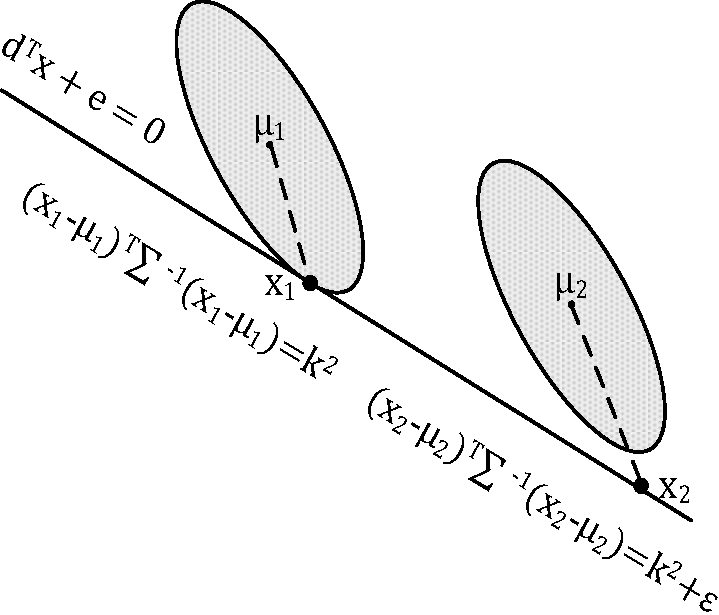
\includegraphics[scale=0.7]{ellipse2.pdf}
\caption{The ellipse centred around $\mu_1$ intersects the constraint while the ellipse centred around $\mu_2$ is wholly above (satisfies) the constraint. The shortest Mahalanobis distance will not necessarily be perpendicular to the constraint.}
\label{fig_mahala_ellipse}
\end{figure}
Since $x$ is a Gaussian stochastic variable we have that $\mathbb{E}[x] =\mu$ and $\text{var}[x]=\Sigma$. Let $\Omega = \{x \in \mathbb{R}^n~|~(x-\mu)^T\Sigma^{-1}(x-\mu) \leq k^2\}$ and $k^2$ be the critical value such that for the Chi Squared distribution with degrees of freedom equal to the dimension of $x$ we have that $\text{Pr}(\mathcal{X} \leq k^2) = p$. Then it is well known \cite{mahala2} that $\int_{\Omega}p(x|\mu, \Sigma)dx = p$ where $p(\cdot|\mu, \Sigma)$ is the multivariate Gaussian probability distribution function of $x$. If the shortest squared Mahalanobis distance from the mean of $x$ is further away from the affine constraint $d^Tz+e=0$ than $k^2$ it implies that the curve of the function $h(z) = (z-\mu)^T\Sigma^{-1}(z-\mu) = k^2$ does not intersect with the constraint - a positive $\epsilon$ in the context of Figure \ref{fig_mahala_ellipse}. Therefore $\Omega$ is wholly contained within the feasible region because $d^T\mu+e> 0 $. This implies, with at least a probability of $p$, that the chance constraint will not be violated because the ``confidence ellipse" is contained in the feasible region. Therefore, by applying Theorem \ref{thrm_mahala_dist} to find the shortest squared Mahalanobis distance between $\mu$ and the constraint we have that $\frac{(d^T\mu+e)^2}{d^T \Sigma d} \geq k^2 \implies \text{Pr}(d^Tx + e \geq 0) \geq p$.

The generalisation to more than one constraint, which should be jointly satisfied, is shown in Figure \ref{fig_mahala_ellipse_joint}. It is required that the ellipse, up to confidence level $p$, is wholly contained in the feasible region $Dx +e >0$. If this requirement is satisfied we will satisfy the joint chance constraint by the same reasoning as before.  
\begin{figure}[H] 
\centering
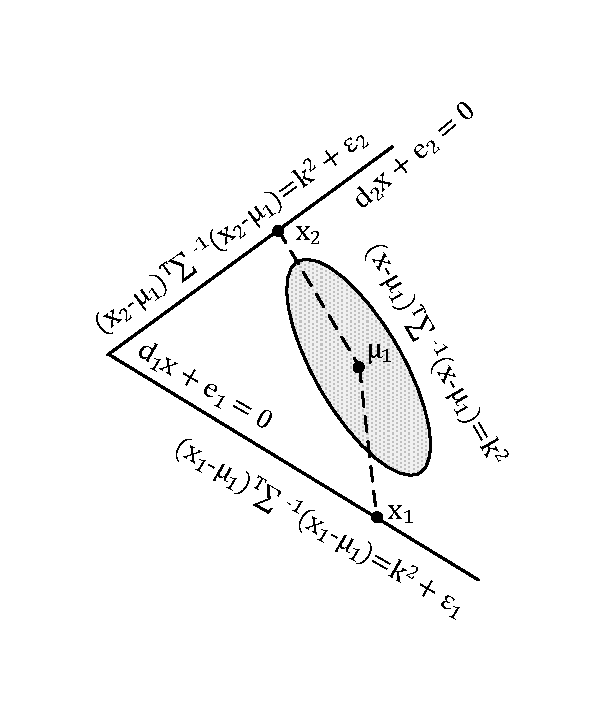
\includegraphics[scale=0.8]{multiple.pdf}
\caption{Illustration of the fact that Theorem \ref{thrm_chance_cons} holds jointly for multiple constraints. The ellipse centred around $\mu$ must lie wholly within the feasible region. This is guaranteed if the Mahalanobis constraint is satisfied.}
\label{fig_mahala_ellipse_joint}
\end{figure}
By ensuring that $D\mu + e > 0$ and that the shortest squared Mahalanobis distance between $\mu$ and the constraints is bigger than $k^2$ this is guaranteed. This implies that if for all $i=1,...,n$ $\frac{(d^T_i\mu+e_i)^2}{d_i^T \Sigma d_i} \geq k^2$ then $\text{Pr}(Dx + e \geq 0) \geq p$ will be satisfied.
\end{proof}
In Theorem \ref{thrm_chance_cons} it is important that $\mu$ lie within the feasible region. If that is not required then it is possible for the ellipse to be wholly outside the feasible region while still satisfying the requirement that the shortest squared Mahalanobis distance between $\mu$ and the constraints is at least $k^2$. Clearly the chance constraint will then not be satisfied. 

It is interesting to note the striking similarity between the work in \cite{vanhessem1} and \cite{vanhessem2} and Theorem \ref{thrm_chance_cons} given that we started analysing the problem within the framework of graphical models. The additional benefit of Theorem \ref{thrm_chance_cons} is that it formulates the chance constraint as a function of the statistical Mahalanobis distance measure. This is useful because it lends a statistical interpretation to Theorem \ref{thrm_chance_cons} even if the underlying distribution is non-Gaussian.

In Theorem \ref{thrm_mpc_stoch_to_det} we combine and elaborate on the work of \cite{yan1}, \cite{vanhessem1} to yield a QP MPC which exactly satisfies the stochastic MPC in (\ref{eq_mpc_constrained_linmod}) given the assumptions of linearity and normality. Note that the dimensionality of the problem is arbitrary.
\begin{thrm}
\textbf{Conversion of the stochastic MPC formulation to the standard deterministic QP MPC formulation} Under the assumptions of linearity and Gaussian distributions we can reformulate the stochastic MPC problem shown in (\ref{eq_mpc_constrained_linmod}) as a standard deterministic QP MPC problem shown in (\ref{eq_mpc_constrained_linmod_deter}).
\begin{equation}
\begin{aligned}
&\underset{\mathbf{u}}{\text{min }} \frac{1}{2}\sum_{k=0}^{N-1} \left( \mu_k^TQ\mu_k + u_k^TRu_k \right) + \frac{1}{2}\mu_N^TP_f\mu_N + \frac{1}{2}\sum_{k=0}^N \text{tr}(Q\Sigma_k) \\
& \text{subject to } \mu_{t+1}=A\mu_t + Bu_t \\
& \text{and } \Sigma_{t+1} = W+A\Sigma_t A^T \\
& \text{and } d^T\mu_t + e \geq k\sqrt{d^T \Sigma_t d} ~\forall ~t=1,...,N\\
\end{aligned}
\label{eq_mpc_constrained_linmod_deter}
\end{equation}
\label{thrm_mpc_stoch_to_det}
Other deterministic constraints, e.g. on the input, can be added as usual. Note that we have assumed that the initial state estimate $x_0$ is available in the form of its mean, $\mu_0$,  and covariance, $\Sigma_0$. It is straightforward to include more chance constraints. Since each chance constraint is reduced to an inequality constraint which measures the Mahalanobis distance between the predicted distributions, the resultant feasible points will jointly satisfy all chance constraints.  
\end{thrm}
\begin{proof}
Let the admissible set of controller inputs $\mathcal{U}$ be the same for both the stochastic MPC and the deterministic MPC formulations. Furthermore, let the current state estimate $x_0$ be given. Then by Theorem \ref{thrm_lqr_lqg_diff} the objective function and equality constraints follow. By Theorem \ref{thrm_affine_expected_const} the expected value inequality constraint in (\ref{eq_mpc_constrained_linmod}) can be reformulated to require that $d^T\mu_t + e \geq 0$ for each $t=1, 2,..., N$. The chance constraint in (\ref{eq_mpc_constrained_linmod}) follows from Theorem \ref{thrm_chance_cons} as shown in (\ref{eq_chance_to_lin}).
\begin{equation}
\begin{aligned}
\frac{(d^T\mu_t+e)^2}{d^T \Sigma_t d} \geq k^2 &\implies (d^T\mu_t+e)^2 \geq k^2 {d^T \Sigma_t d} \\
&\implies d^T\mu_t+e \geq k \sqrt{d^T \Sigma_t d}~\forall~t=1, 2,..., N
\end{aligned}
\label{eq_chance_to_lin}
\end{equation}
The first line of (\ref{eq_chance_to_lin}) follows because $\Sigma_t$ is positive semi-definite for all $t=1, 2,..., N$ and $d \neq 0$ (otherwise it would not be a constraint), therefore it can be multiplied over the inequality sign like a positive number. By Theorem \ref{thrm_lqg_sol} we have that $\Sigma_{t+1} = W + A\Sigma_tA^T$, therefore the predicted covariance matrices used in (\ref{eq_chance_to_lin}) are well defined. The second line follows because of the first inequality constraint: we know that $d^T\mu_t+e \geq 0 ~\forall~t=1,2,..., N$ and therefore we can square root both sides of the inequality constraint. Thus we have the two inequality constraints $d^T\mu_t+e \geq 0$ and $d^T\mu_t+e \geq k \sqrt{d^T \Sigma_t d}$ for each $t=1,2,...,N$. Since $k > 0$ (otherwise we do not have a meaningful chance constraint) we can condense the two inequality constraints into a single constraint: $d^T\mu_t+e \geq k \sqrt{d^T \Sigma_t d} > 0$ for each $t=1,2,...,N$ from which the conclusion follows.  
\end{proof}
The beauty of Theorem \ref{thrm_mpc_stoch_to_det} is that no new theory is necessary to analyse the stability and convergence results of the new MPC. This is highly desirable because it allows one to merely ``add" the inequality constraint in (\ref{eq_mpc_constrained_linmod_deter}) to your existing MPC formulation. Most practical MPCs will have some form of state estimation and thus no new parameters are introduced either. Since the problem is in standard QP form it is straightforward to implement and, even more importantly, it is computationally fast because the problem is trivially convex.

In the work by \cite{yan1} and \cite{yan2}, which primarily dealt with univariate problems, it was found that feasibility problems might arise if one uses the predicted covariance estimates in the controller. If the system is unstable the uncertainty in the estimates can grow with time as discussed in Theorem \ref{thrm_lqg_sol_inf}. This can cause the ellipses used in Theorem \ref{thrm_chance_cons} to become too large to fit inside the feasible region. The approach adopted by \cite{yan1} and \cite{yan2} is to only use the one step ahead predicted covariance ($\Sigma_1$) over the entire prediction horizon. This does not ensure feasibility but restricts the growth associated with infeasibility. The drawback of this approach is that it might cause constraint violation because the controller will be more aggressive.  

\section{Reference tracking}
So far we have only dealt with controllers which drive the system to the origin. The more general situation we are interested in is arbitrary reference point tracking. Fortunately, Chapter \ref{sec_lit_ref_track} applies without modification because the stochastic MPC problem was reduced to the \textit{standard} deterministic MPC problem. 

\section{Linear system}
\label{sec_lin_sys_cont}
In this chapter we consider the problem of controlling a linear system using the stochastic MPC formulation of Theorem \ref{thrm_mpc_stoch_to_det}. More precisely, we assume the linear model linearised about the unsteady operating point of our CSTR example from Chapter \ref{sec_cstr} accurately represents the underlying system. For the purposes of illustration we will only use the (somewhat unrealistic) system where both states are measured. However, there is no theoretical reason why we cannot use the system where only temperature is measured. The drawback of using the latter system is that inference, as discussed previously, will be worse. The control goal is to steer the concentration, in the sense of Definition \ref{def_stoch_ref_track_goal}, to the unsteady operating point ($C_A = 0.49$ kmol.m$^{-3}$) about which the system was linearised. See Chapter \ref{sec_cstr} for more details.

We repeat the relevant system dynamics in (\ref{eq_linmod_params}) using a time step $h=0.1$. 
\begin{equation}
\begin{aligned}
&A = \begin{pmatrix}
0.9959 & -6.0308\times 10^{-5} \\
0.4186 & 1.0100
\end{pmatrix}
~~B = \begin{pmatrix}
0 \\ 8.4102\times 10^{-5}
\end{pmatrix} ~~
C = \begin{pmatrix}
1 & 0 \\ 0 & 1
\end{pmatrix} \\
&W = \begin{pmatrix}
1\times 10^{-6} & 0 \\ 0 & 0.1
\end{pmatrix} ~~
V = \begin{pmatrix}
1\times 10^{-3} & 0 \\ 0 & 10
\end{pmatrix}
\end{aligned}
\label{eq_linmod_params}
\end{equation}
The tuning parameters used in this and all subsequent chapters are shown in (\ref{eq_mpc_tuning}). Note that the magnitude difference between the components of $Q$, $P_f$ and $R$ is necessary because the units of concentration and heat input are not scaled. 
\begin{equation}
\begin{aligned}
Q = P_f = \begin{pmatrix}
1\times 10^{4} & 0 \\ 0 & 0
\end{pmatrix} 
~~R = \begin{pmatrix}
1\times 10^{-6}
\end{pmatrix}
\end{aligned}
\label{eq_mpc_tuning}
\end{equation}
We assume that a Kalman filter supplies the current posterior state estimate $x_0$ at each time step. Additionally, we assume a zero order hold of 1 min between controller inputs.

It is useful to introduce the measures we will use to quantify the effectiveness of the control techniques used in this and the following chapters. We define the average energy input by $\frac{1}{N}\sum^N_{t=0}|u_t-u_s|$ and the average concentration error by $\frac{1}{N}\sum^N_{t=0}|\frac{{C_A}_t-y_{sp}}{y_{sp}}|$. Additionally, to confirm that the results hold true over multiple simulations we will, at the end of Chapters \ref{sec_lin_sys_cont} and \ref{sec_nonlinear_control}, include a Monte-Carlo simulation. The metrics we use for the Monte Carlo simulations will be the time each simulation spent in violation of the constraints and the total state space area (measured within the context of the Mahalanobis distance) in violation of the constraint. 

First we illustrate the approach of using only the result of Theorem \ref{thrm_lqg_sol} i.e. we apply the LQG regulator to the system. Based on our previous results we know that given the Kalman filter's current posterior state estimate mean, $\mu_0$, we only need to solve the LQR as shown in (\ref{eq_lqg_linmod}) to solve the LQG problem. The prediction horizon $N$ is set at 150 time steps i.e. 15 minutes into the future. 
\begin{equation}
\begin{aligned}
&\underset{\mathbf{u}}{\text{min }} \frac{1}{2}\sum_{k=0}^{N-1} \left( \mu_k^TQ\mu_k + u_k^TRu_k \right) + \frac{1}{2}\mu_N^TP_f\mu_N \\
& \text{subject to } \mu_{t+1}=A\mu_t + Bu_t \\
\end{aligned}
\label{eq_lqg_linmod}
\end{equation}
Figure \ref{fig_lin_mod_lqg} shows that the system does indeed converge, noisily, to the set point. This is not surprising because we have effectively just implemented the very well studied LQG controller. The primary drawback of this method is that there is no easy way to constrain the system. From a practical perspective this can be problematic. 
\begin{figure}[H] 
\centering
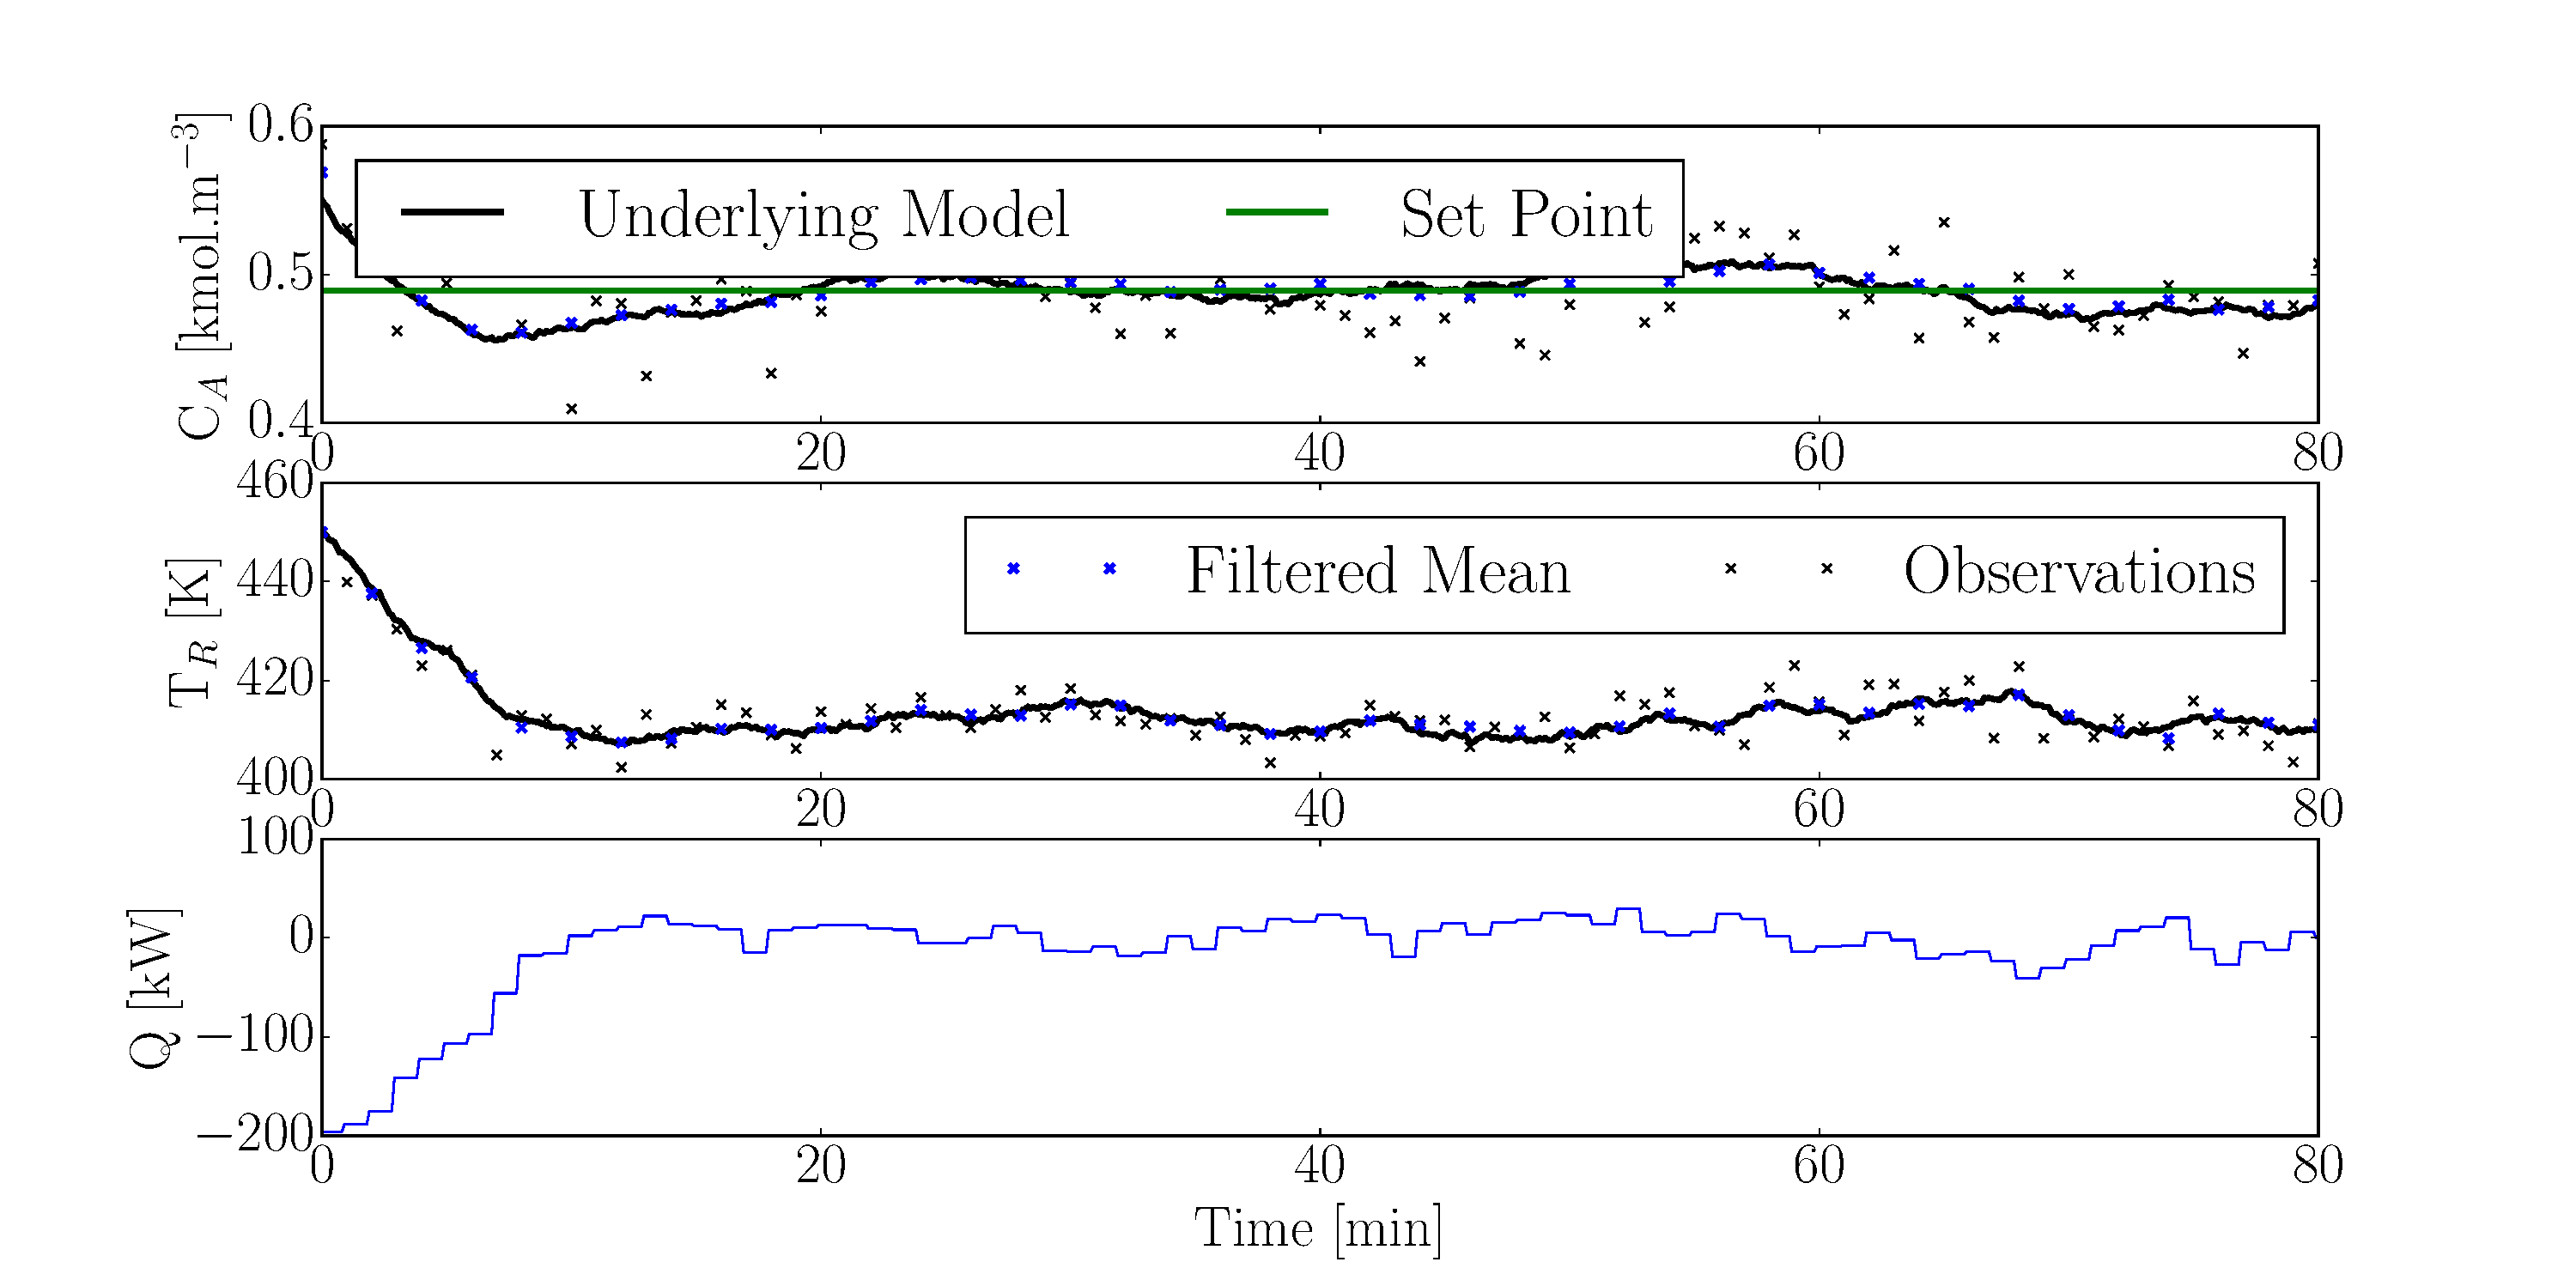
\includegraphics[width=\textwidth]{lin_mod_lqg.pdf}
\caption{Unconstrained LQG regulator tracking with initial condition $(0.55, 450)$ and measuring both states.}
\label{fig_lin_mod_lqg}
\end{figure}
The average heat energy usage (controller input) over the simulation run is 24.99 kW. The average set point error is 2.29\% over the same 80 min time period.
 
Next we illustrate the approach of using conventional deterministic MPC to control the stochastic system. The MPC formulation is shown in (\ref{eq_mpc_constrained_det1}). Using MPC allows us to easily add state and input constraints; this is a significant improvement over conventional LQG as discussed previously.
\begin{equation}
\begin{aligned}
&\underset{\mathbf{u}}{\text{min }} \frac{1}{2}\sum_{k=0}^{N-1} \left( \mu_k^TQ\mu_k + u_k^TRu_k \right) + \frac{1}{2}\mu_N^TP_f\mu_N \\
& \text{subject to } \mu_{t+1}=A\mu_t + Bu_t \\
&\text{and } \begin{pmatrix}
10 \\ 1
\end{pmatrix}^T \mu_t + 412 \geq 0 ~\forall ~t=1,...,N\\
& \text{and } |u_t| \leq 165 ~\forall ~t=0,...,N-1\\
\end{aligned}
\label{eq_mpc_constrained_det1}
\end{equation}
We only use a single state constraint in this dissertation but the extension to multiple constraints is straightforward. The prediction and control horizon are equal to each other and set at 150 time steps i.e. 15 minutes into the future. We additionally constrain the magnitude of the inputs.

Due to assumption of normality and linearity and by Theorem \ref{thrm_lqg_sol} and \ref{thrm_affine_expected_const} we can also interpret the deterministic MPC as a stochastic MPC with an affine expected value constraint. Therefore the controller in (\ref{eq_mpc_constrained_det1}) is not inappropriate for the control of the stochastic CSTR process under consideration.

In Figure \ref{fig_lin_mod_kf_mean_track} we see the reference tracking and controller input for the deterministic MPC. The average heat energy input and set point error over the simulation run is 28.22 kW and 2.43\% respectively. Interestingly the average error is not much different but the controller requires more energy to track the set point. This is reasonable because the additional constraints make problem (\ref{eq_mpc_constrained_det1}) a harder problem than (\ref{eq_lqg_linmod}).
\begin{figure}[H] 
\centering
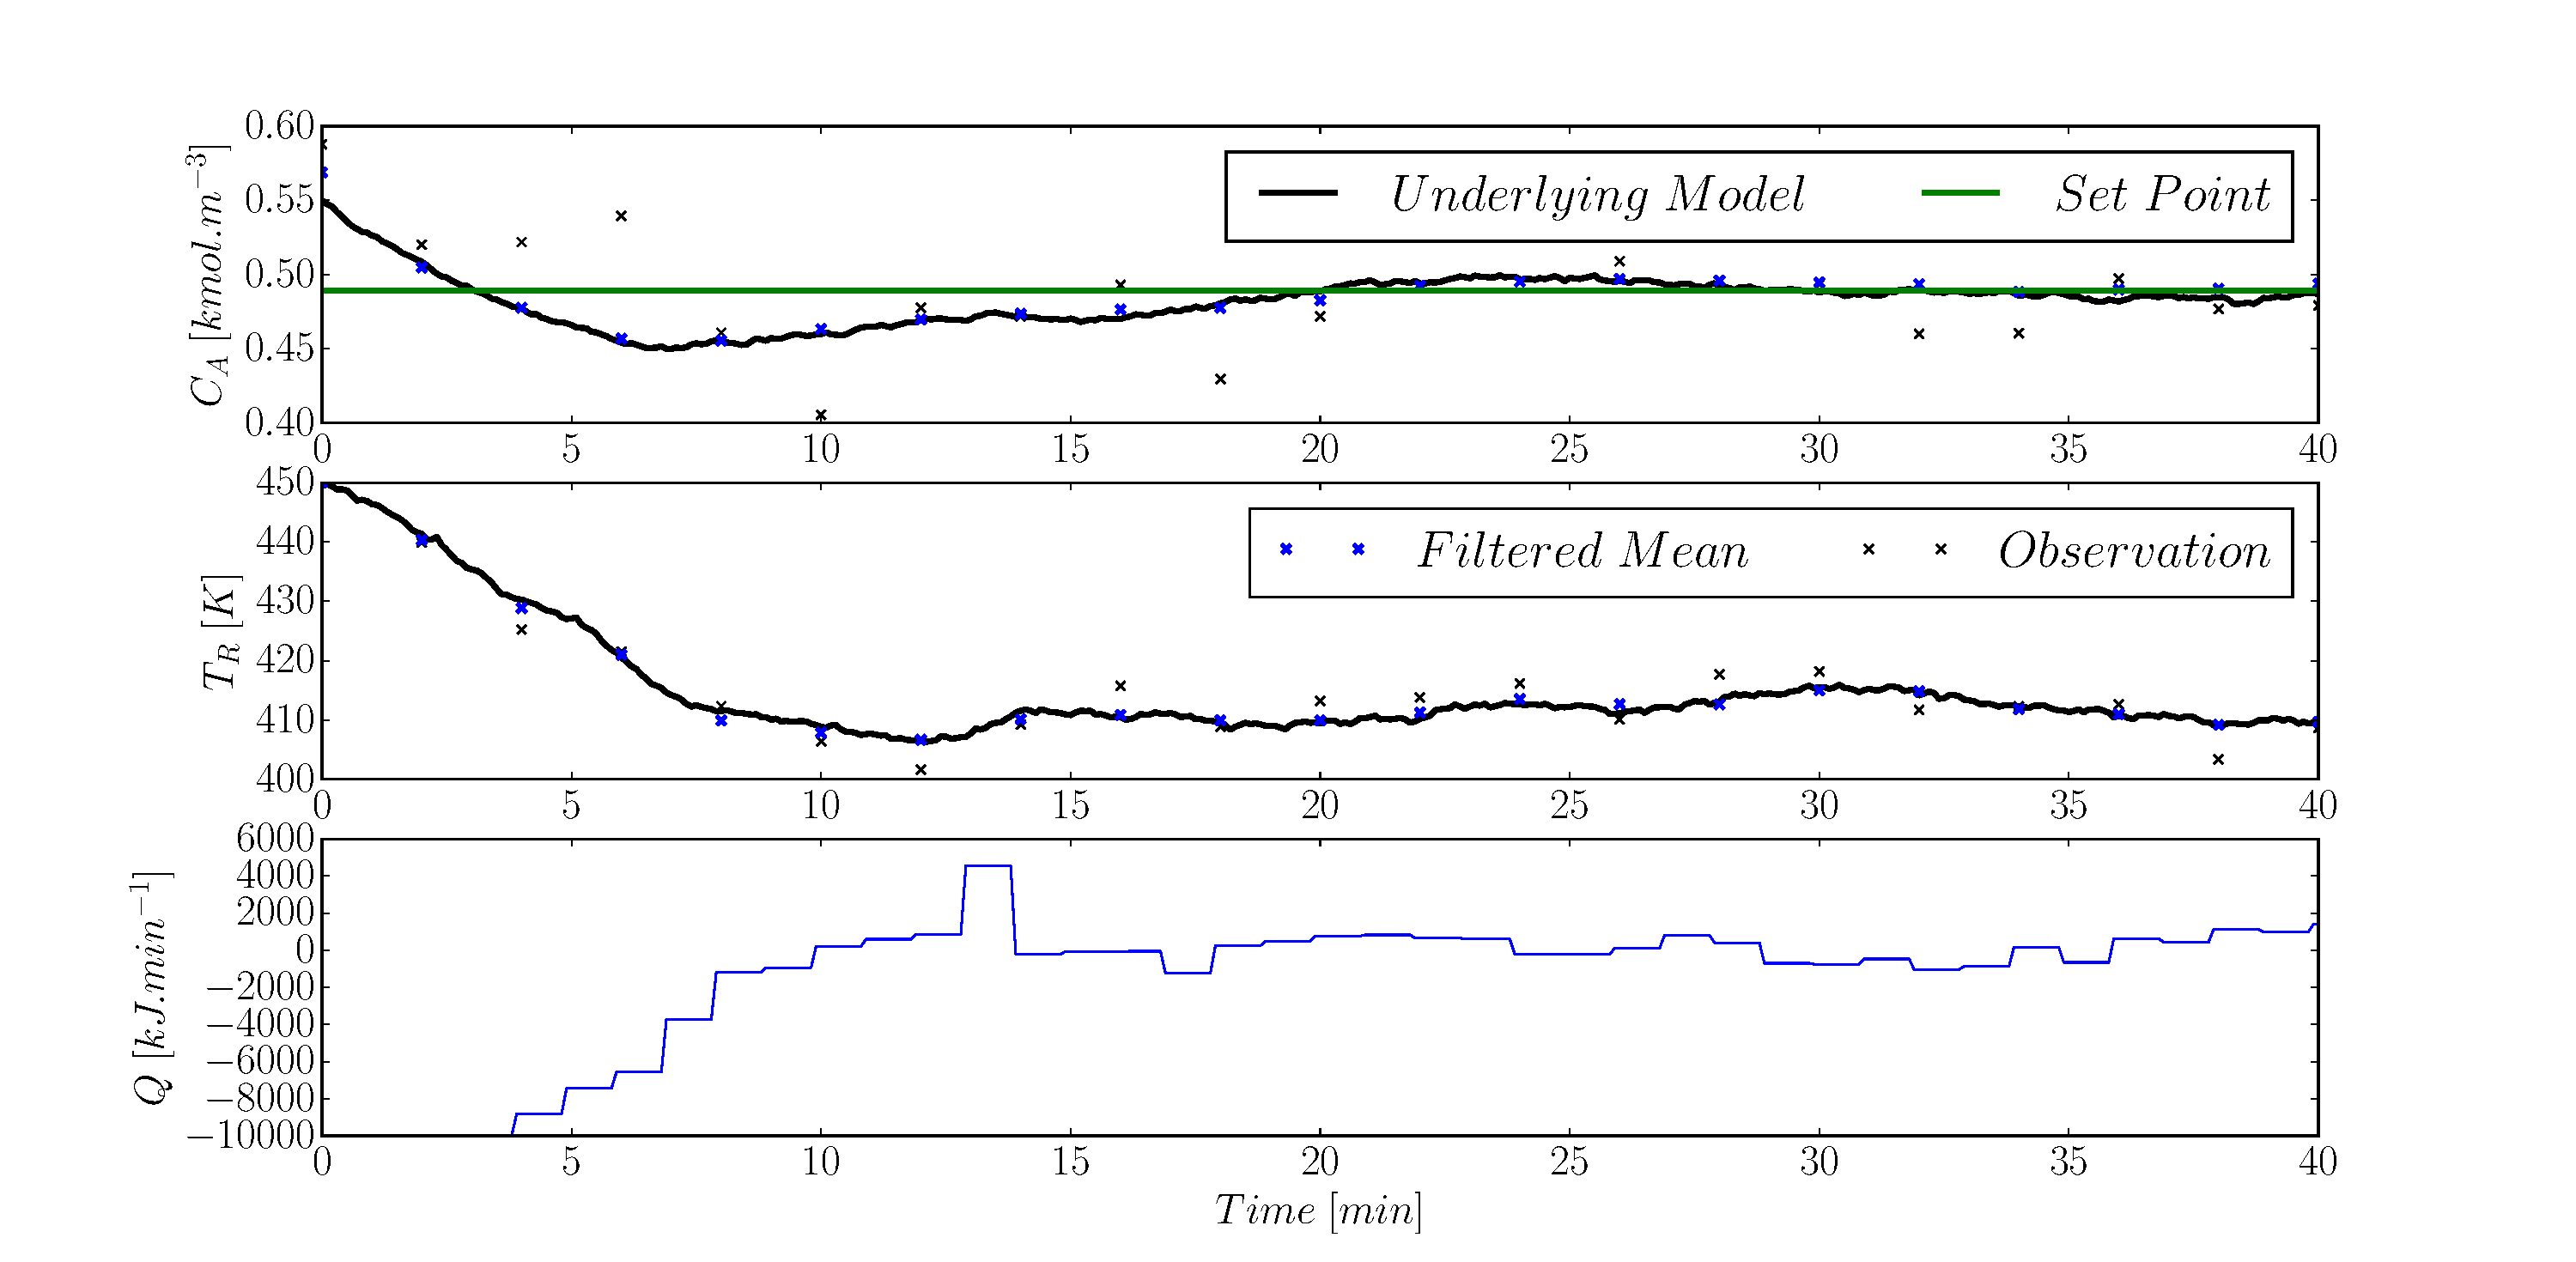
\includegraphics[width=\textwidth]{lin_mod_kf_mean_track.pdf}
\caption{Deterministic constrained MPC tracking with initial condition $(0.55, 450)$ and measuring both states.}
\label{fig_lin_mod_kf_mean_track}
\end{figure}
Like the LQG controller, it is clear that we have noisy convergence to the set point. As mentioned previously we will never be able to achieve zero set point offset because of the noise term in the system dynamics (\ref{eq_lin_system}). Note that we have constrained the maximum magnitude of the inputs such that $|u_t| \leq 165$ kW. In the unconstrained case the controller required a maximum absolute input magnitude of over $200$ kW; the ability to naturally constrain the inputs can be practically very useful. The benefit of MPC is apparent here.

In Figure \ref{fig_lin_mod_kf_mean_ss} we see the corresponding state space trajectory of the system together with the state constraint.
\begin{figure}[H]
\centering
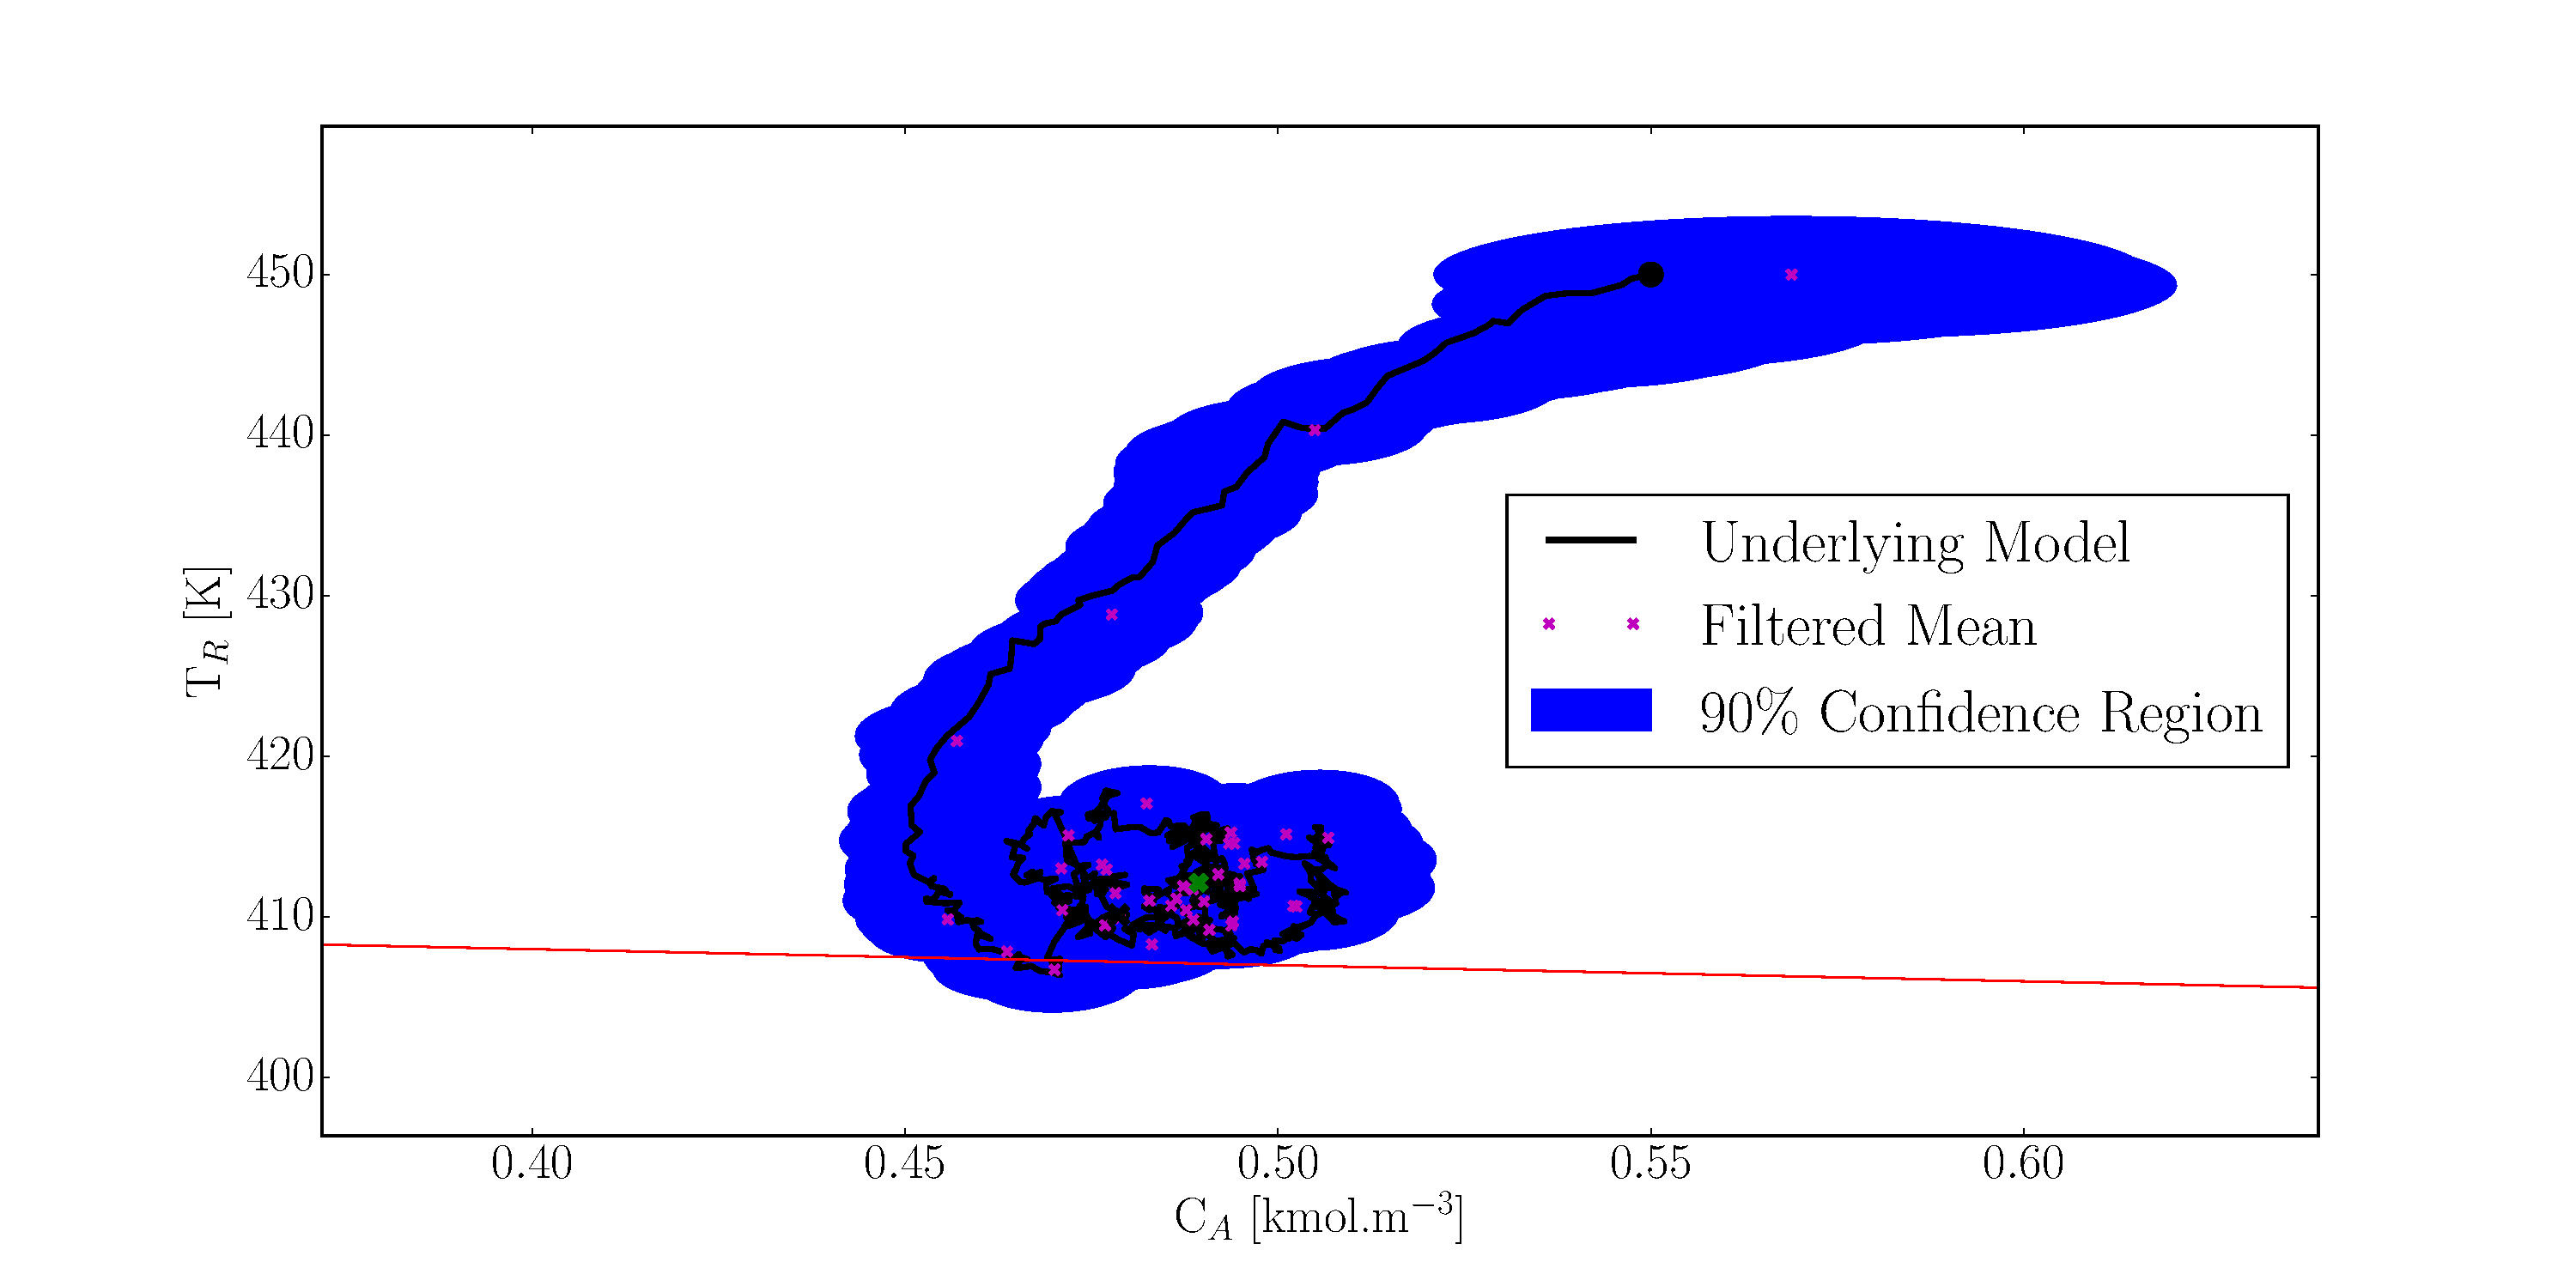
\includegraphics[width=\textwidth]{lin_mod_kf_mean_ss.pdf}
\caption{Deterministic MPC state space trajectory with initial condition $(0.55, 450)$ and measuring both states.}
\label{fig_lin_mod_kf_mean_ss}
\end{figure}
While the predicted mean state estimates do not violate the constraint (due to the optimisation constraints) the actual underlying system does.  This is clearly seen if one inspects the confidence region around the lower state estimates in Figure \ref{fig_lin_mod_kf_mean_ss}. The confidence region is deeply violated by the constraint which implies that it is likely that the underlying system might. This is clearly a problem from a control point of view; the deterministic MPC cannot ensure that the constraint is satisfied.

We remedy this situation by introducing the chance constrained MPC as discussed in Theorem \ref{thrm_mpc_stoch_to_det} and shown in (\ref{eq_mpc_linmod_kf_cons}) for convenience. Note that $d^T = (10, 1)$ and $e=412$ as before. By consulting a Chi Squared distribution table we set $k^2 = 4.6052$ which corresponds to the chance constraint $\text{Pr}(d^Tx_t + e \geq 0) \geq 90\% ~\forall ~t=1,...,N$.
\begin{equation}
\begin{aligned}
&\underset{\mathbf{u}}{\text{min }} \frac{1}{2}\sum_{k=0}^{N-1} \left( \mu_k^TQ\mu_k + u_k^TRu_k \right) + \frac{1}{2}\mu_N^TP_f\mu_N + \frac{1}{2}\sum_{k=0}^N \text{tr}(Q\Sigma_k) \\
& \text{subject to } \mu_{t+1}=A\mu_t + Bu_t \\
& \text{and } \Sigma_{t+1} = W+A\Sigma_t A^T \\
& \text{and } d^T\mu_t + e \geq k\sqrt{d^T \Sigma_t d} ~\forall ~t=1,...,N\\
& \text{and } |u_t| \leq 165 ~\forall ~t=0,...,N-1\\
\end{aligned}
\label{eq_mpc_linmod_kf_cons}
\end{equation}
Note that problem (\ref{eq_mpc_linmod_kf_cons}) is harder than (\ref{eq_mpc_constrained_det1}) due to the added constraint and thus we expect that the system will require greater controller input to satisfy the constraint. 

In Figure \ref{fig_lin_mod_kf_var90_track} we see that the stochastic MPC is able to track the set point in a similar manner as the LQG controller and deterministic MPC. The total average heat input and set point error over the simulation run is  38.58 kW and 2.58\% respectively. This problem is harder than the preceding one due to the additional constraint and thus more energy is required. 
\begin{figure}[H] 
\centering
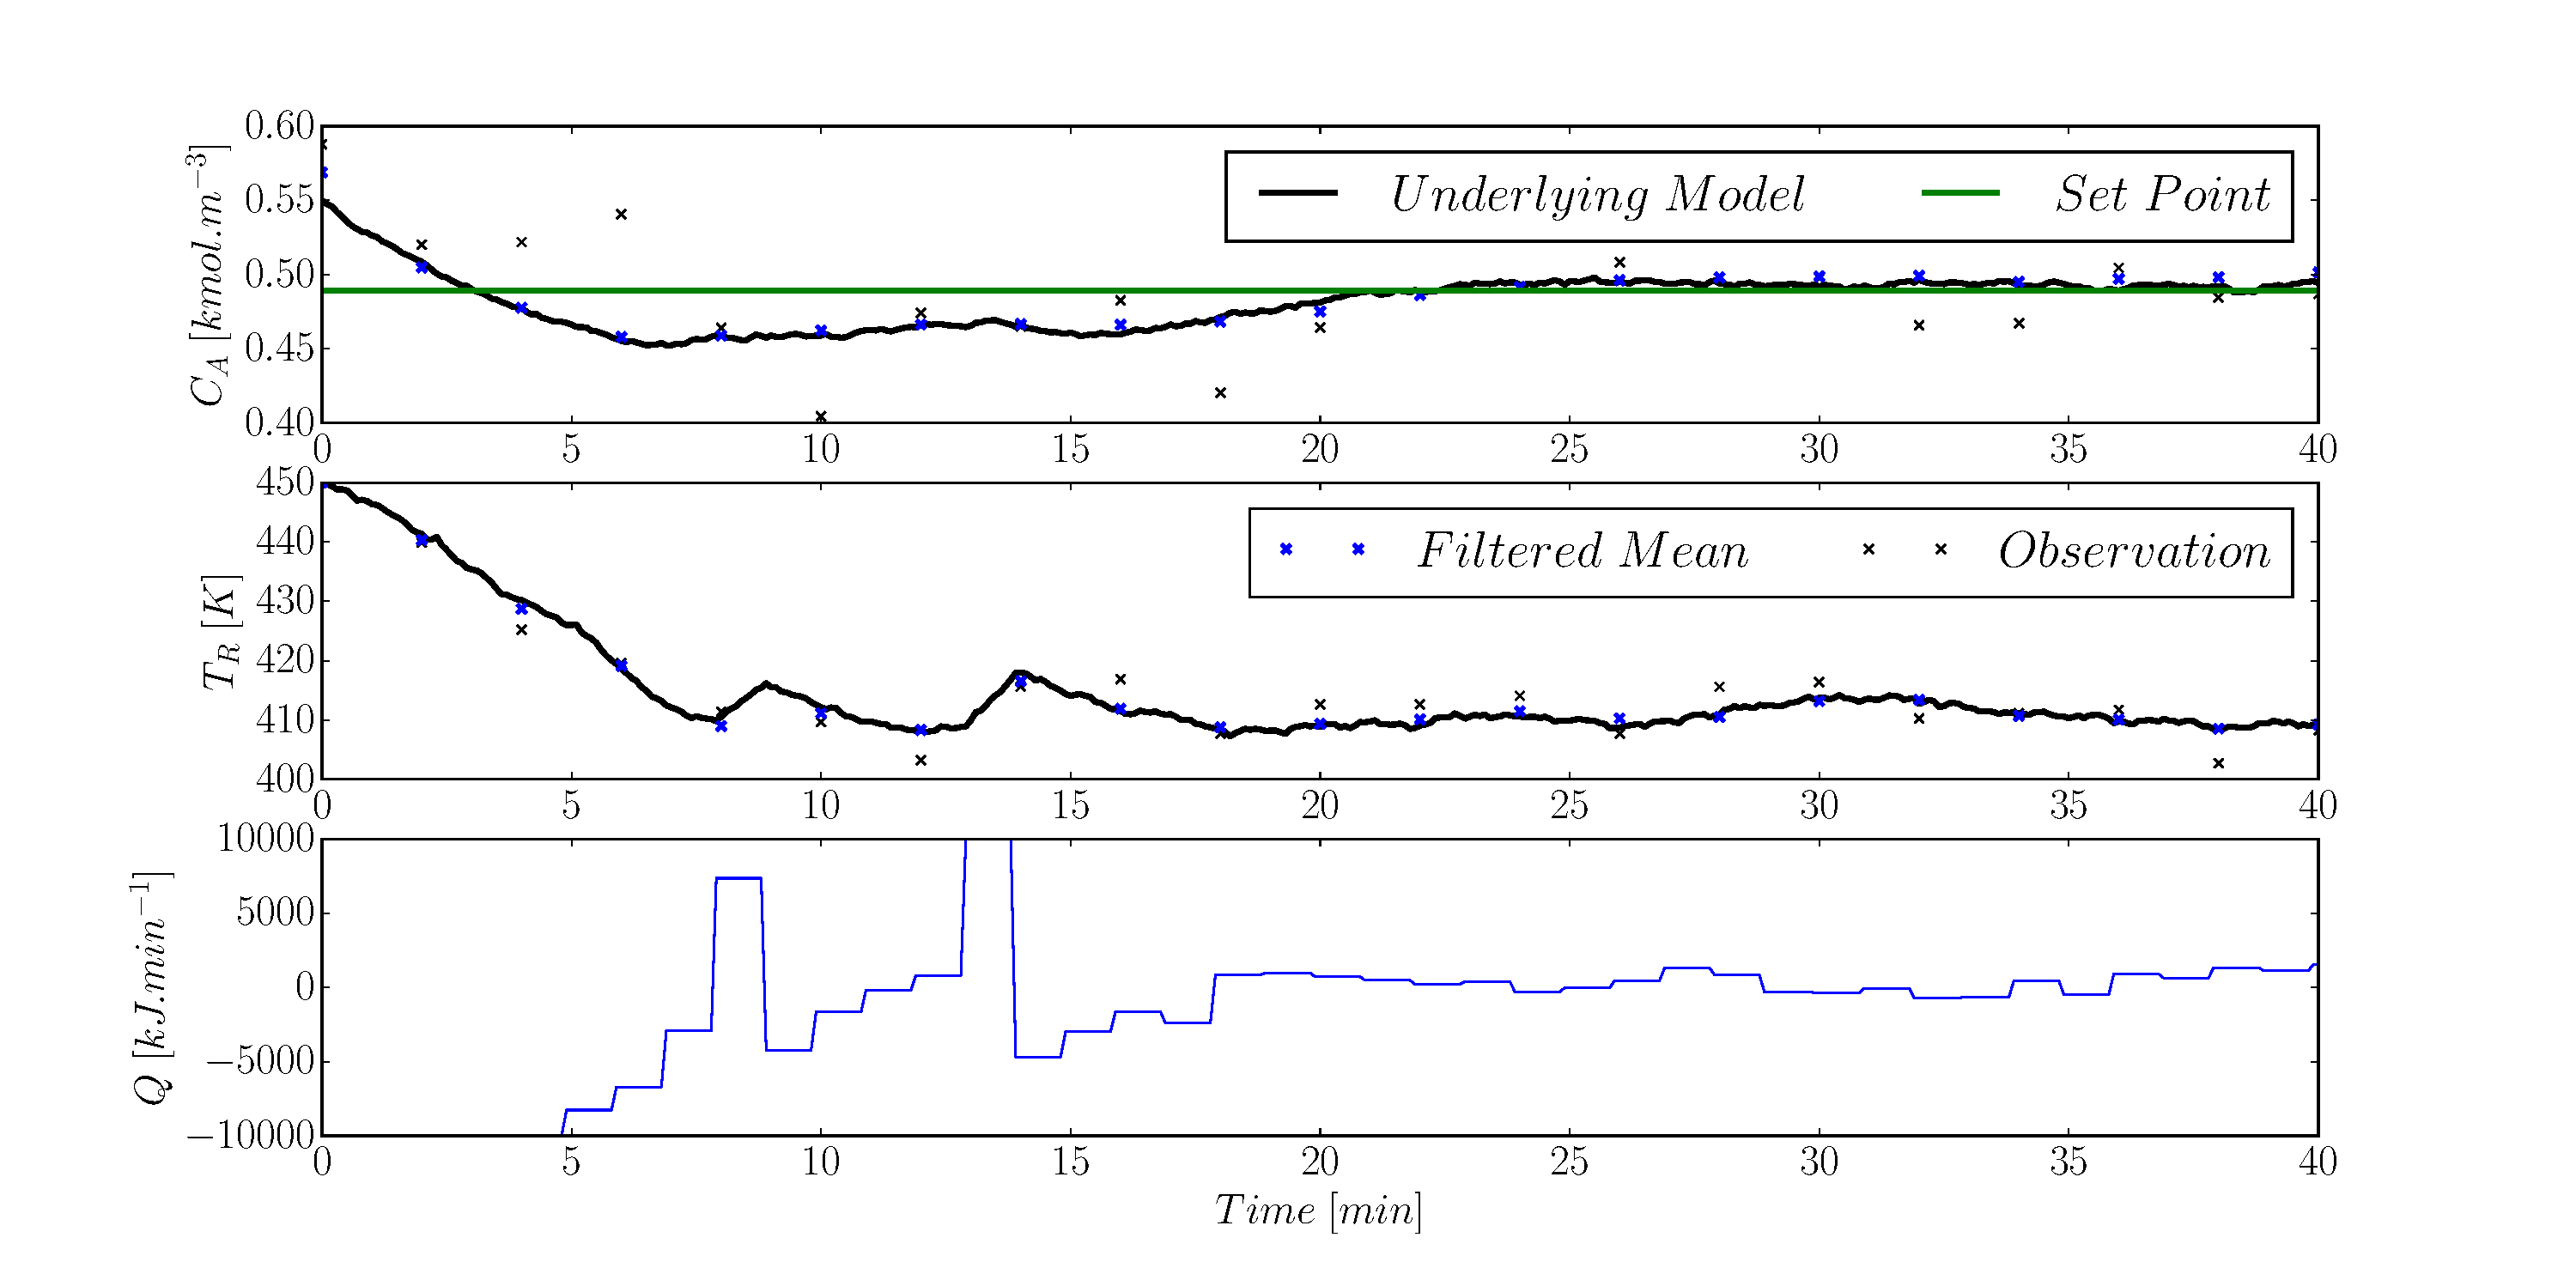
\includegraphics[width=\textwidth]{lin_mod_kf_var90_track.pdf}
\caption{Chance constrained MPC tracking with initial condition $(0.55, 450)$ and measuring both states. A Kalman filter is used for inference and the chance constraint is set at 90\%.}
\label{fig_lin_mod_kf_var90_track}
\end{figure}
However, the benefit of adding the chance constraint is apparent in Figure \ref{fig_lin_mod_kf_var90_ss}. It is clear that the constraint on the underlying state is not violated.
\begin{figure}[H] 
\centering
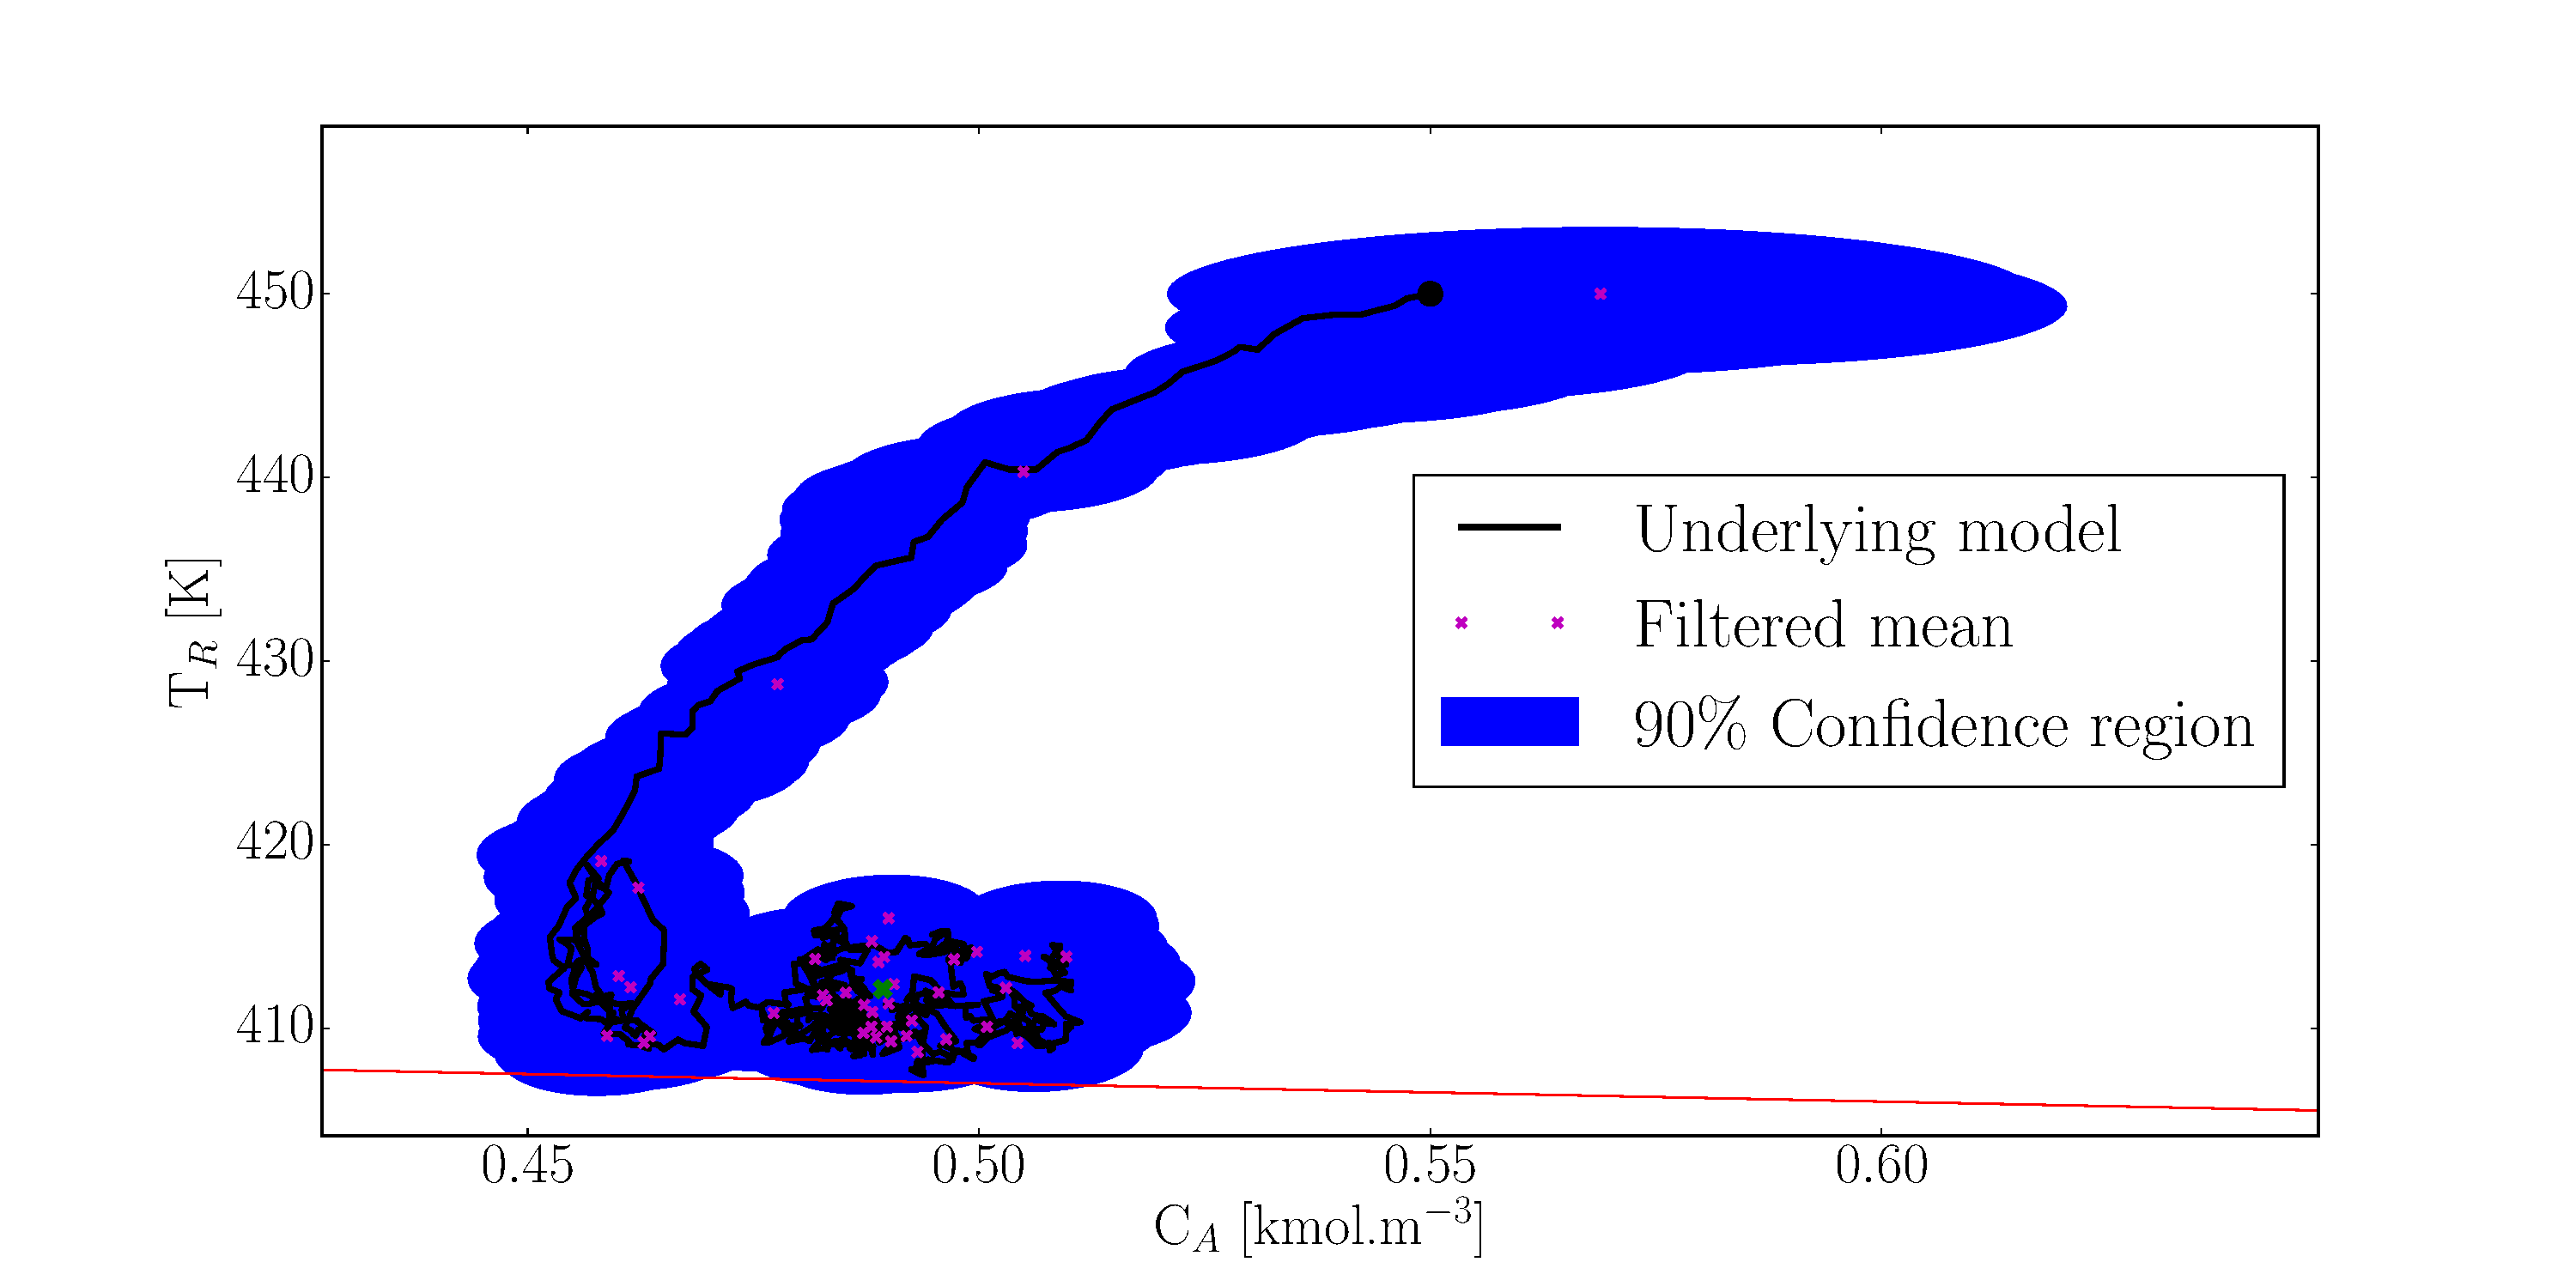
\includegraphics[width=\textwidth]{lin_mod_kf_var90_ss.pdf}
\caption{Chance constrained MPC state space trajectory with initial condition $(0.55, 450)$ and measuring both states. A Kalman filter is used for inference and the chance constraint is set at 90\%.}
\label{fig_lin_mod_kf_var90_ss}
\end{figure}
Since the chance constraint is only enforced with probability 90\% it is possible that the underlying system can come ``close" to the constraint. This then has the consequence that the posterior confidence region marginally violates (spills over) the constraint as seen in the lower regions of Figure \ref{fig_lin_mod_kf_var90_ss}.
 
It is interesting to investigate what effect increasing the probability that the chance constraint is satisfied will have on the system. To this end we modify the chance constraint of (\ref{eq_mpc_linmod_kf_cons}) such that $k^2 = 9.21$ which corresponds to the chance constraint $\text{Pr}(d^Tx_t + e \geq 0) \geq 99\% ~\forall ~t=1,...,N$. We expect that the underlying system will be moved further away from constraint due to this added level of conservativeness.

In Figure \ref{fig_lin_mod_kf_var99_track} we see that the stochastic MPC still tracks the set point and Figure \ref{fig_lin_mod_kf_var99_ss} shows that the expected behaviour is realised. 
\begin{figure}[H] 
\centering
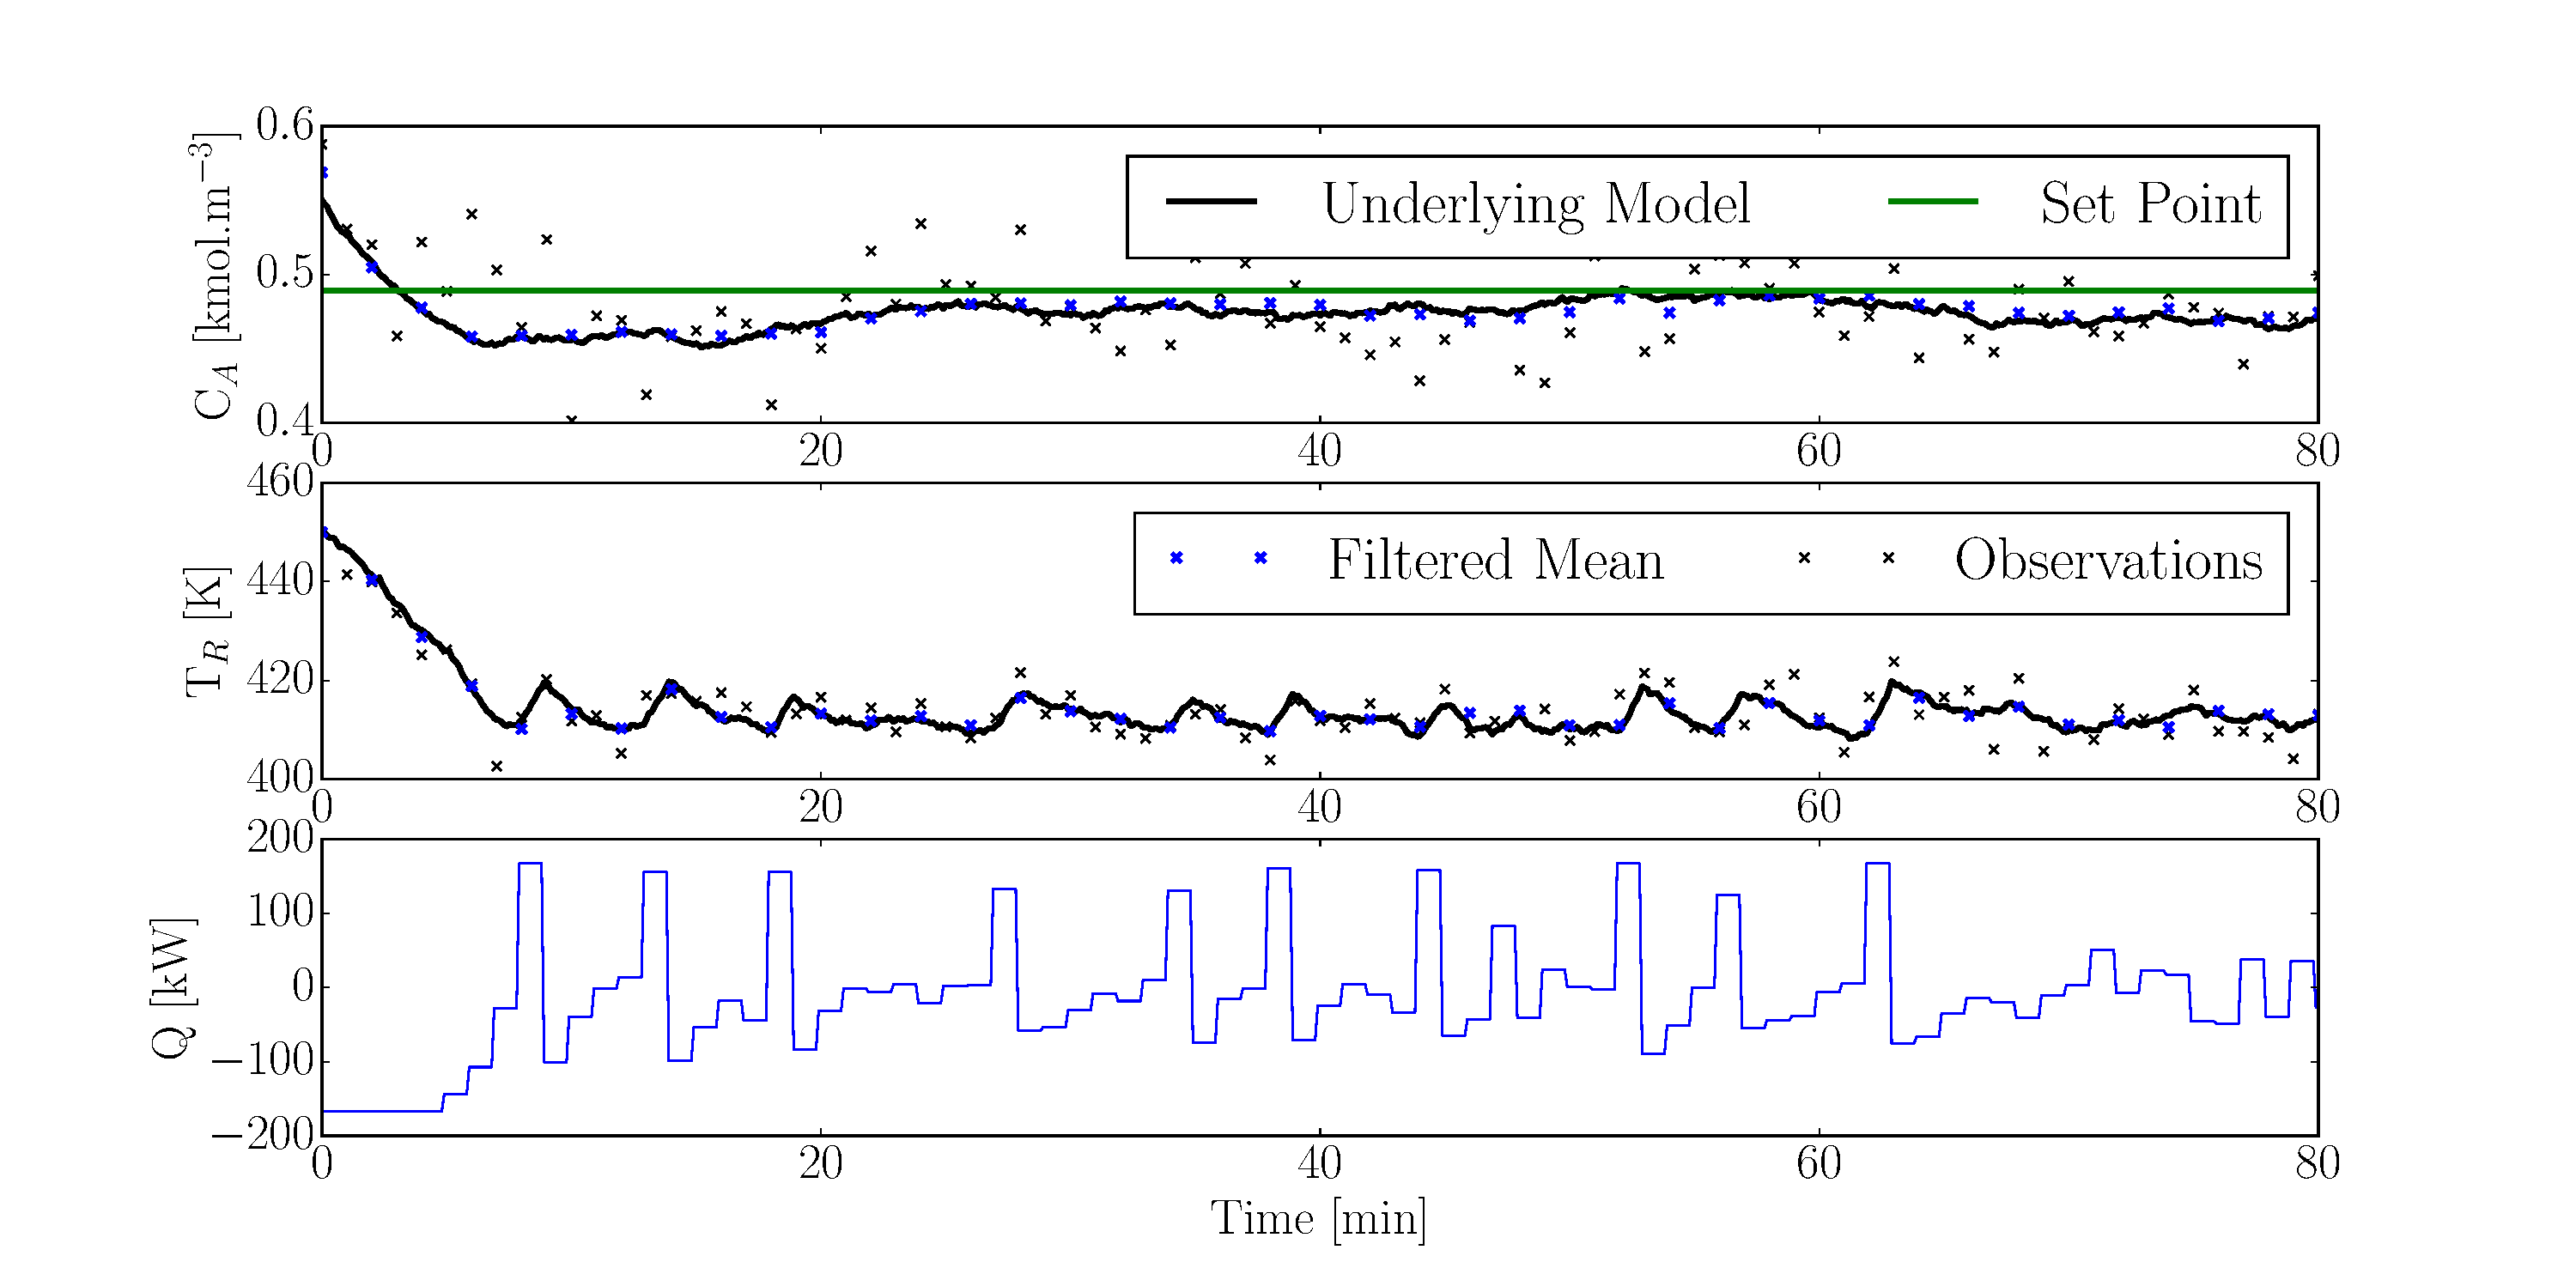
\includegraphics[width=\textwidth]{lin_mod_kf_var99_track.pdf}
\caption{Chance constrained MPC tracking with initial condition $(0.55, 450)$ and measuring both states. A Kalman filter is used for inference and the chance constraint is set at 99\%.}
\label{fig_lin_mod_kf_var99_track}
\end{figure}
The average heat input and average set point error is 3.49\% and  58.39 kW. The added conservativeness of the MPC prevents it from attempting to get to the set point as fast as the previous stochastic MPC; consequently there is no set point overshoot in Figure \ref{fig_lin_mod_kf_var99_track}. This causes the higher average error but the constraints are satisfied more robustly. As before, the control problem is harder and thus requires more energy.

In Figure \ref{fig_lin_mod_kf_var99_ss} we see the 90\% confidence region is above the constraint. Since the probability that the predicted states are close to the constraint is much lower than before we see that the confidence region satisfies the constraint more robustly.
\begin{figure}[H] 
\centering
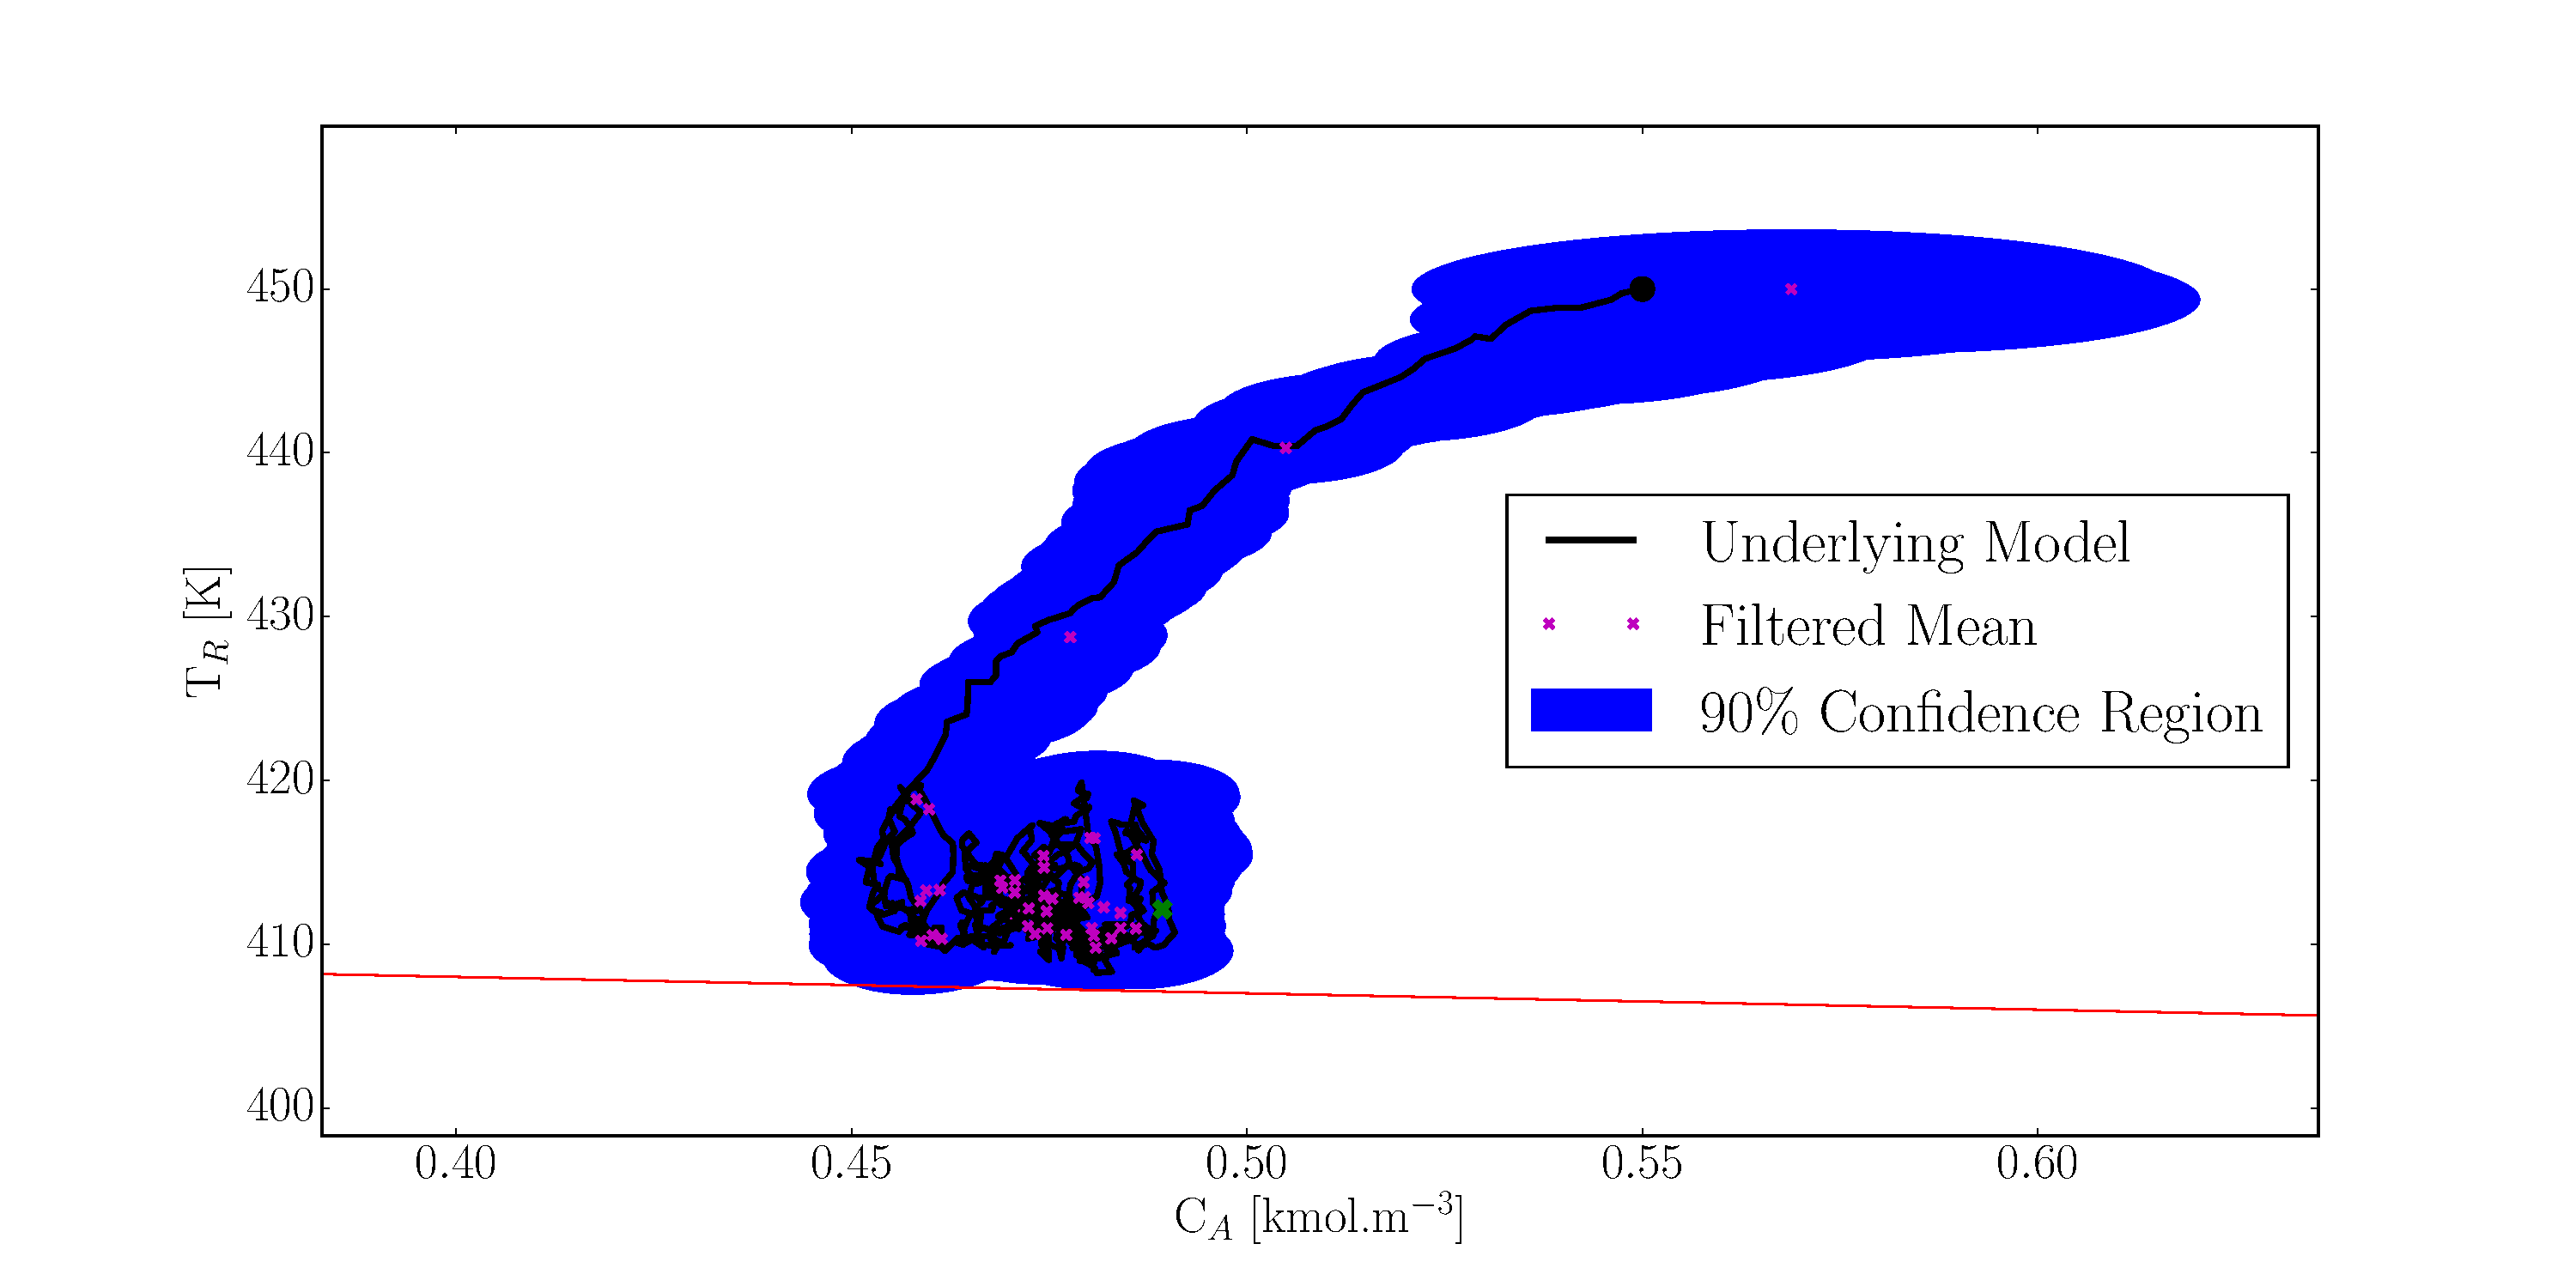
\includegraphics[width=\textwidth]{lin_mod_kf_var99_ss.pdf}
\caption{Chance constrained MPC state space trajectory with initial condition $(0.55, 450)$ and measuring both states. A Kalman filter is used for inference and the chance constraint is set at 99\%.}
\label{fig_lin_mod_kf_var99_ss}
\end{figure}
It would also be correct to infer that $k$ can be used as an empirical measure of the inherent stochastic conservativeness of the resulting controller. That is, lower values of $k$ indicate a more aggressive controller which may violate the chance constraints and higher values of $k$ indicate a more conservative controller. This can be useful for systems where the normal assumption is not valid but one would still like to enforce chance constraints in some empirical sense. 

We have made the strong assumption that the system dynamics remain linear and Gaussian even under the MPC control law which is not necessarily linear \cite{mac}. Clearly if the system is far from Gaussian the Gaussian approach to simplifying the chance constraint will not be valid. Fortunately this is relatively simple to check and serves as a good way of measuring controller health. That is, the more Gaussian the filtered distributions are, the better the linear stochastic controller will work. 

Kullback-Leibler Divergence was introduced in Theorem \ref{thrm_kl_sample} to estimate the degree to which samples match a given distribution. From Chapter \ref{sec_inf_nonlin_mods} we know that given enough particles a particle filter can accurately represent any distribution. Thus we temporarily replace the Kalman filter with a particle filter and use Theorem \ref{thrm_kl_sample} to estimate the degree of normality of the posterior state distributions.

Figure \ref{fig_lin_mod_kl} shows the degree to which the underlying distribution is Gaussian. Since we cannot use an infinite number of particles we compare the sampled Gaussian distribution approximation to a baseline.   
\begin{figure}[H] 
\centering
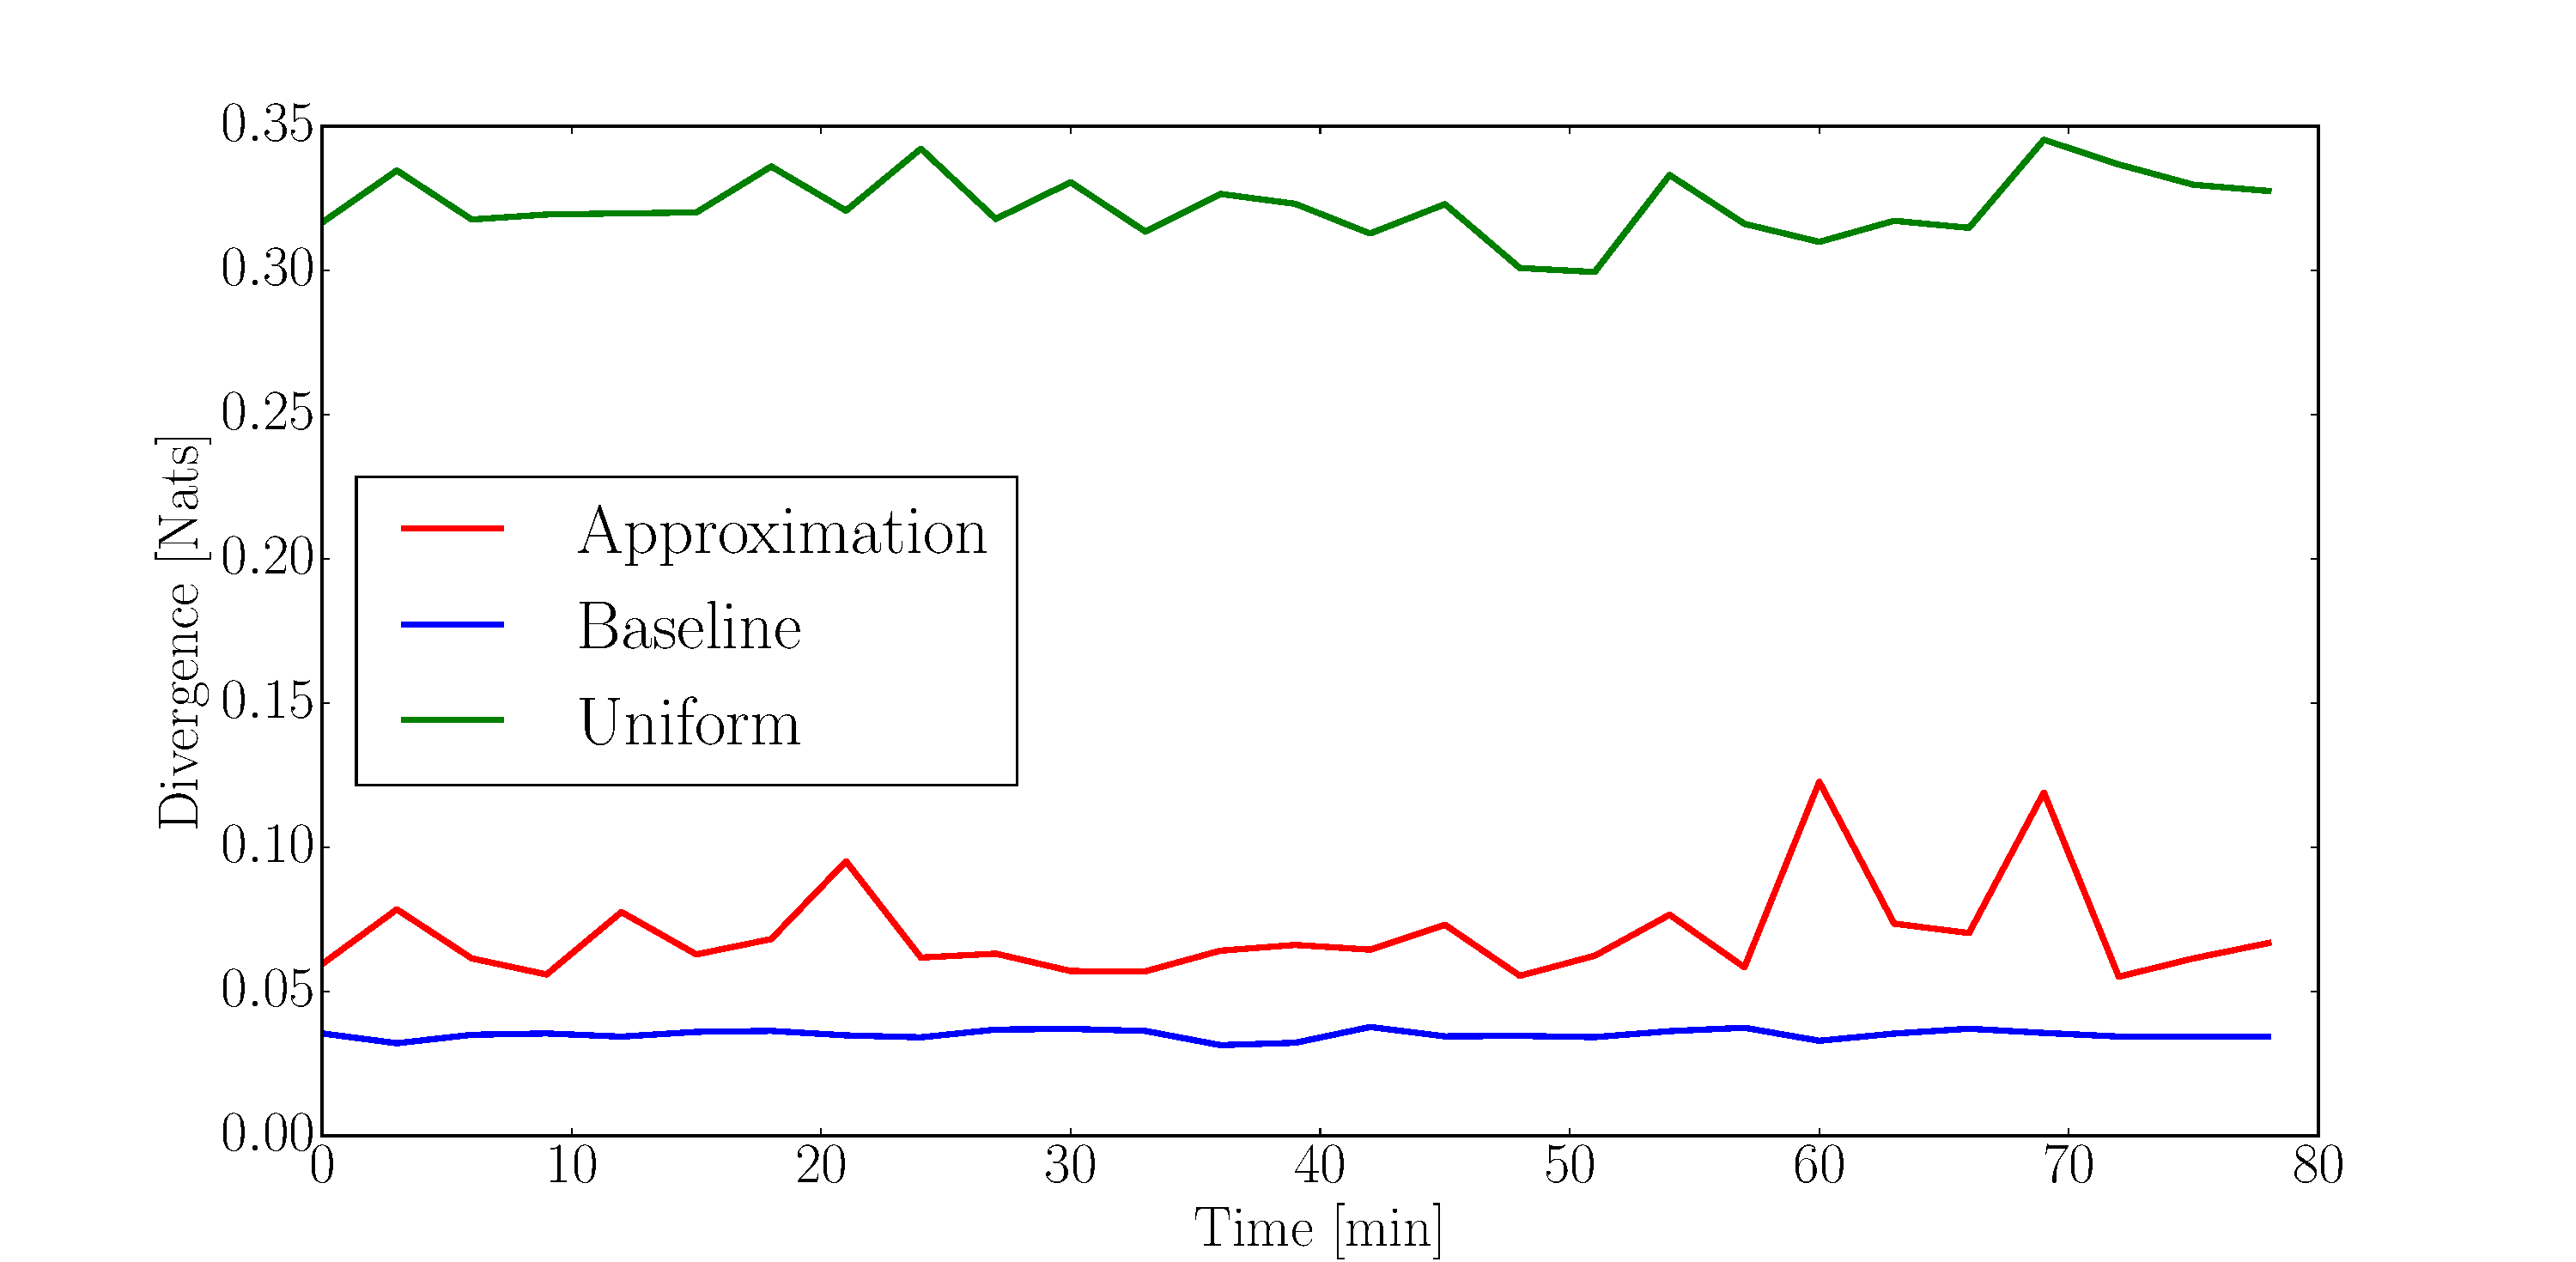
\includegraphics[width=\textwidth]{lin_mod_kl.pdf}
\caption{Kullback-Leibler Divergence between the assumed Gaussian distribution and different sampled distributions using 5000 particles. The underlying model is linear.}
\label{fig_lin_mod_kl}
\end{figure}
The approximation curve in Figure \ref{fig_lin_mod_kl} shows how much the samples diverge from the Gaussian distribution approximated using the samples. The baseline curve shows how much the Gaussian distribution diverges from samples of the same distribution. The uniform curve shows how much a Gaussian approximation of a Uniform distribution drawn in the interval $(\mu_i-2\sigma_{ii}, \mu_i+2\sigma_{ii})$ (for each $i$ in the dimension of the underlying distribution) diverges; this serves to illustrate the divergence one would expect if attempting to model a distribution which is decidedly not normal. One would expect the baseline curve to tend to zero as the number of particles tends to infinity. Sampling error causes divergence from zero for the baseline curve. Thus we can use the baseline and uniform curves as a crude measure of normality.

In Figure \ref{fig_lin_mod_kl} we see that the approximation is relatively close to the baseline. Additionally it is far removed from the uniform curve. The average divergence for the baseline, approximation and uniform curve (in nats) is: $0.035$, $0.069$ and $0.322$ respectively. This implies that even though we are using a non-linear control technique the posterior state distributions are still approximately Gaussian. 

Finally, in Figure \ref{fig_lin_mod_kf_mc} we investigate the effect $k^2$ has on the chance constraint. We expect that by increasing $k^2$ the system becomes more conservative and less likely to violate the constraint. Under the assumptions of linearity and normality we are assured of this behaviour due to Theorem \ref{thrm_mpc_stoch_to_det}. However, as Figure \ref{fig_lin_mod_kl} indicates our assumptions do not  strictly hold. In Figures \ref{fig_lin_mod_kf_var90_ss} and \ref{fig_lin_mod_kf_var99_ss} we reached the conclusion that the chance constraint was effective by only considering a single simulation. In Figure \ref{fig_lin_mod_kf_mc} we show the compilation of over 2000 runs to illustrate the veracity of the claim that the chance constraints are effective.
\begin{figure}[H] 
\centering
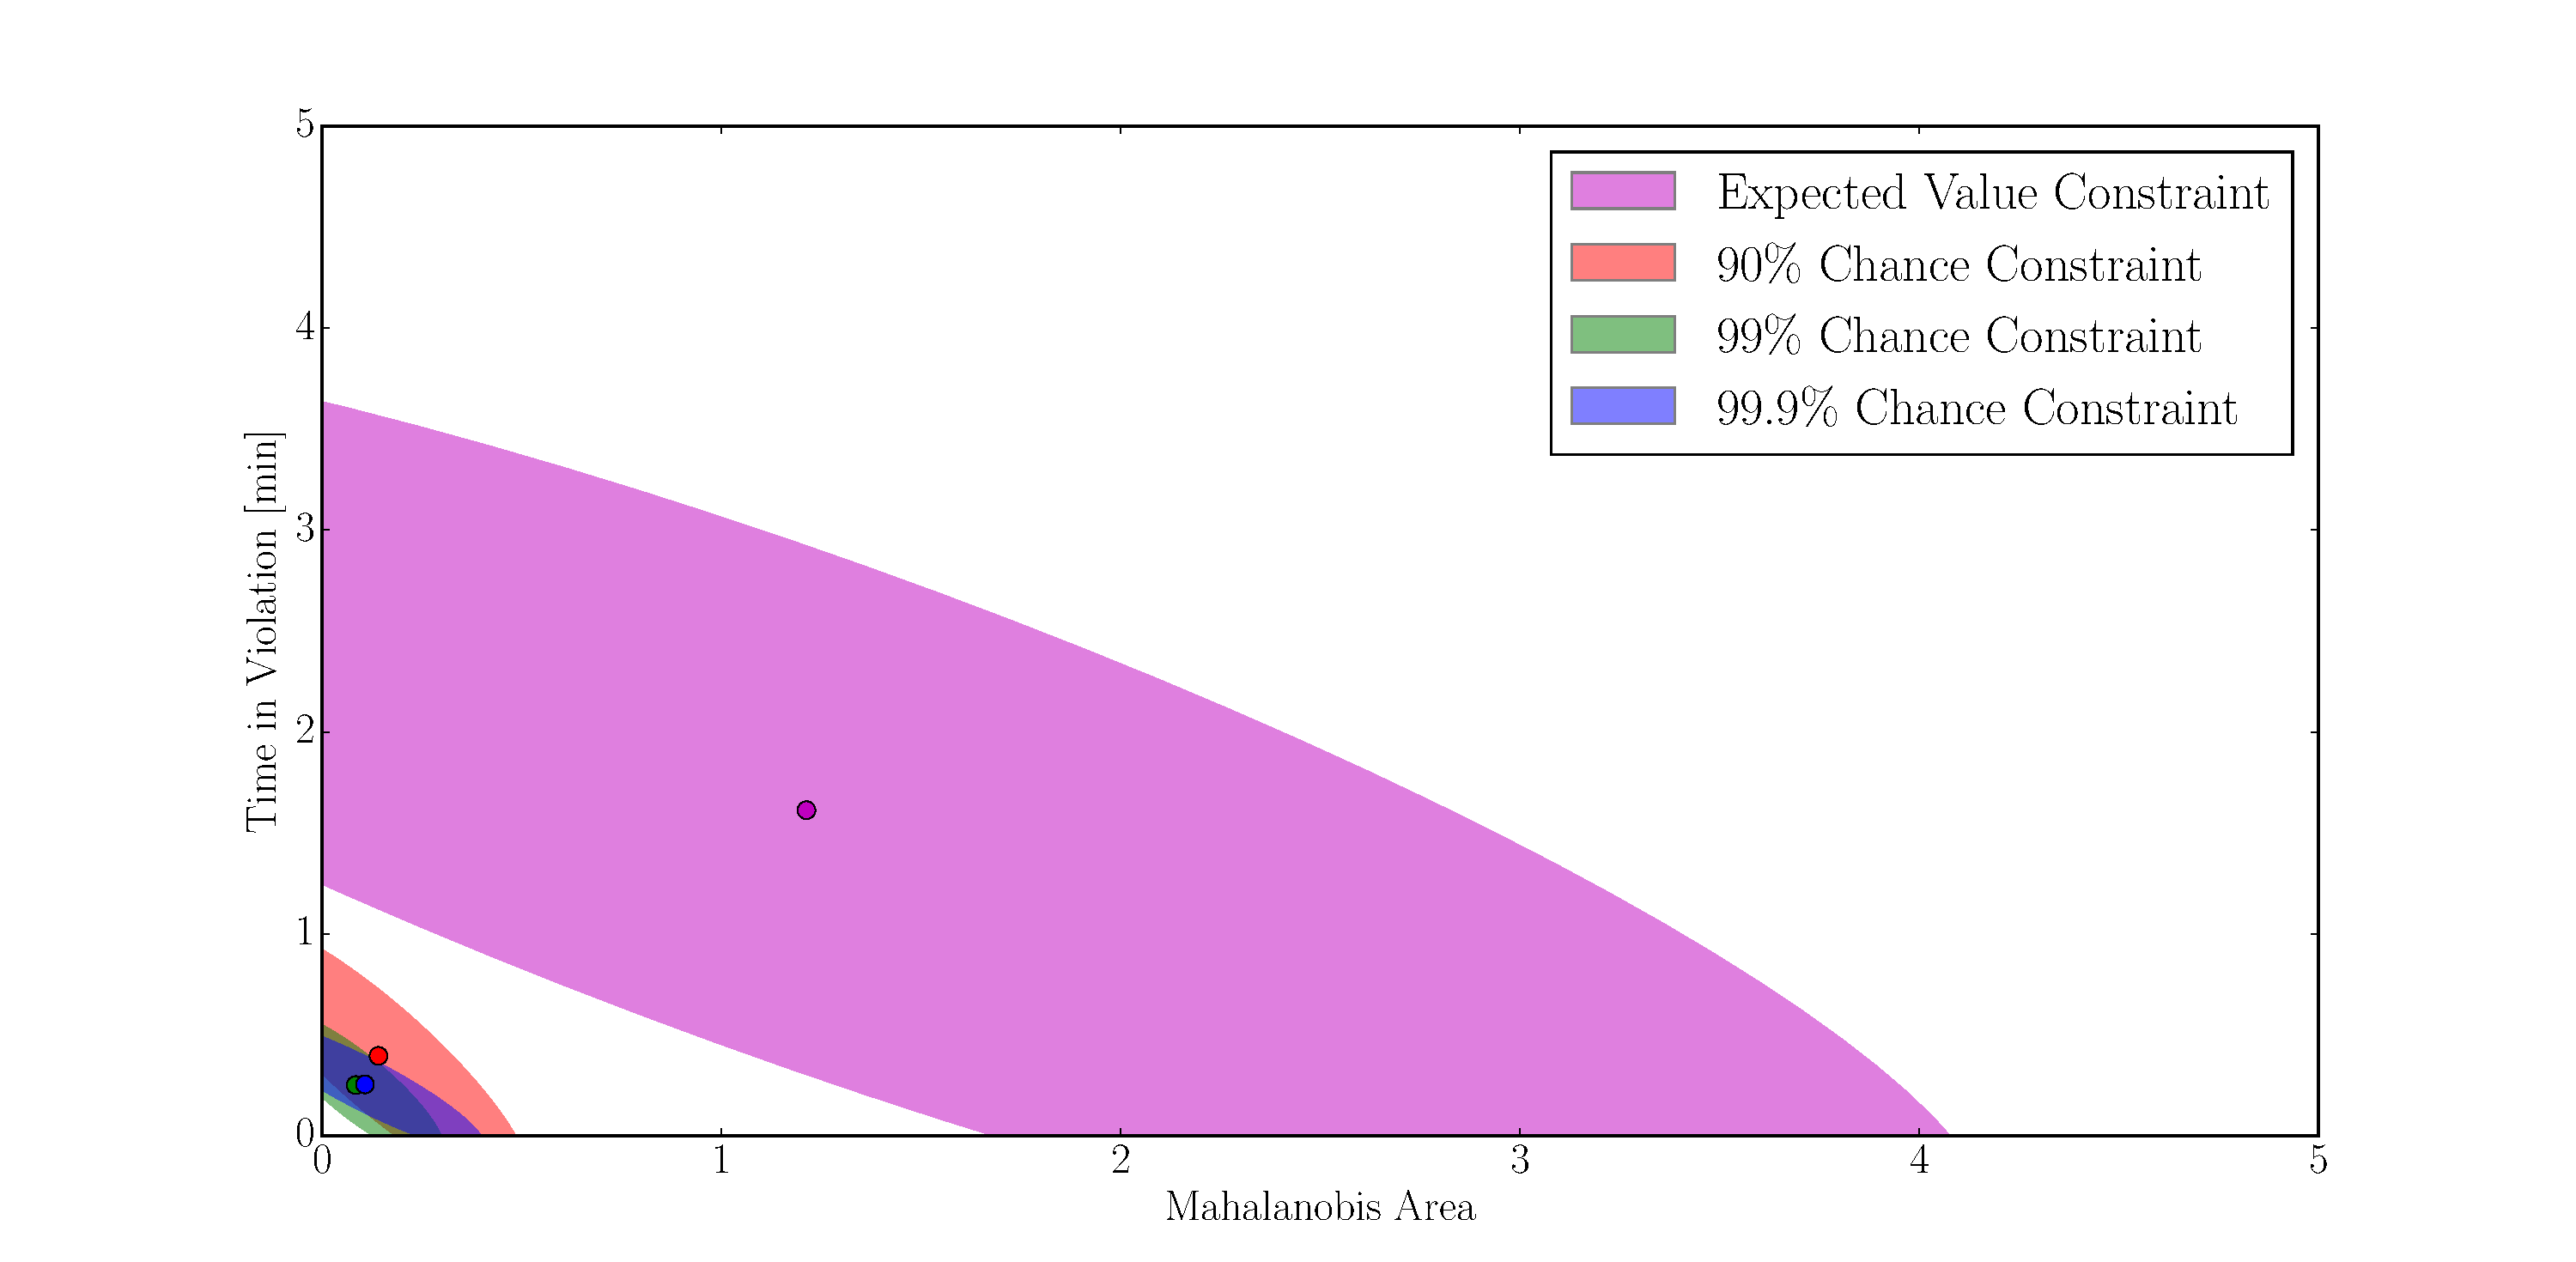
\includegraphics[width=\textwidth]{lin_mod_kf_mc.pdf}
\caption{Monte-Carlo simulation to investigate the effect increasing $k^2$ has on the constraint violation characteristics of the MPC controllers. Each region indicates where 90\% of the simulations scored. The mean is indicated by a solid point.}
\label{fig_lin_mod_kf_mc}
\end{figure}
The Mahalanobis area dimension indicates the degree to which the constraint was violated: larger numbers imply the constraint was deeply violated in state space. The time in violation dimension indicates the length of time the system violated the constraint. It is clear that the chance constraints dramatically reduce the violation characteristics of the system. 

Interestingly, there seems to be diminishing returns on increasing $k^2$ beyond the 99\% chance interval. Feasibility issues plague the system under the more conservative chance constraint levels. Intuitively the predicted ellipses become too big to fit inside the feasible region - especially when projected forward in time. Given that the controller input - the only way to move them inside the feasible region - is constrained the system reaches a performance deadlock. In the work by \cite{yan1} they also noted this problem and solved it by not letting the confidence ellipses grow as they were projected into the future (see the discussion after Theorem \ref{thrm_lqg_sol_inf} and in Chapter \ref{sec_switch_mpc_lit}). For this system the issue is not severe enough to warrant further concern.   

\section{Nonlinear system}
\label{sec_nonlinear_control}
In this chapter we consider the problem of controlling the full non-linear system with a linear model linearised around the unsteady operating point. The control goal is the same as before; the only difference between this chapter and chapter \ref{sec_lin_sys_cont} is that the underlying plant is non-linear.

The linear control model and noise parameters are the same as (\ref{eq_linmod_params}). The control tuning parameters are the same as (\ref{eq_mpc_tuning}).

As before we first investigate the LQG controller. Figure \ref{fig_nonlin_lqg} shows the unconstrained reference tracking results.
\begin{figure}[H] 
\centering
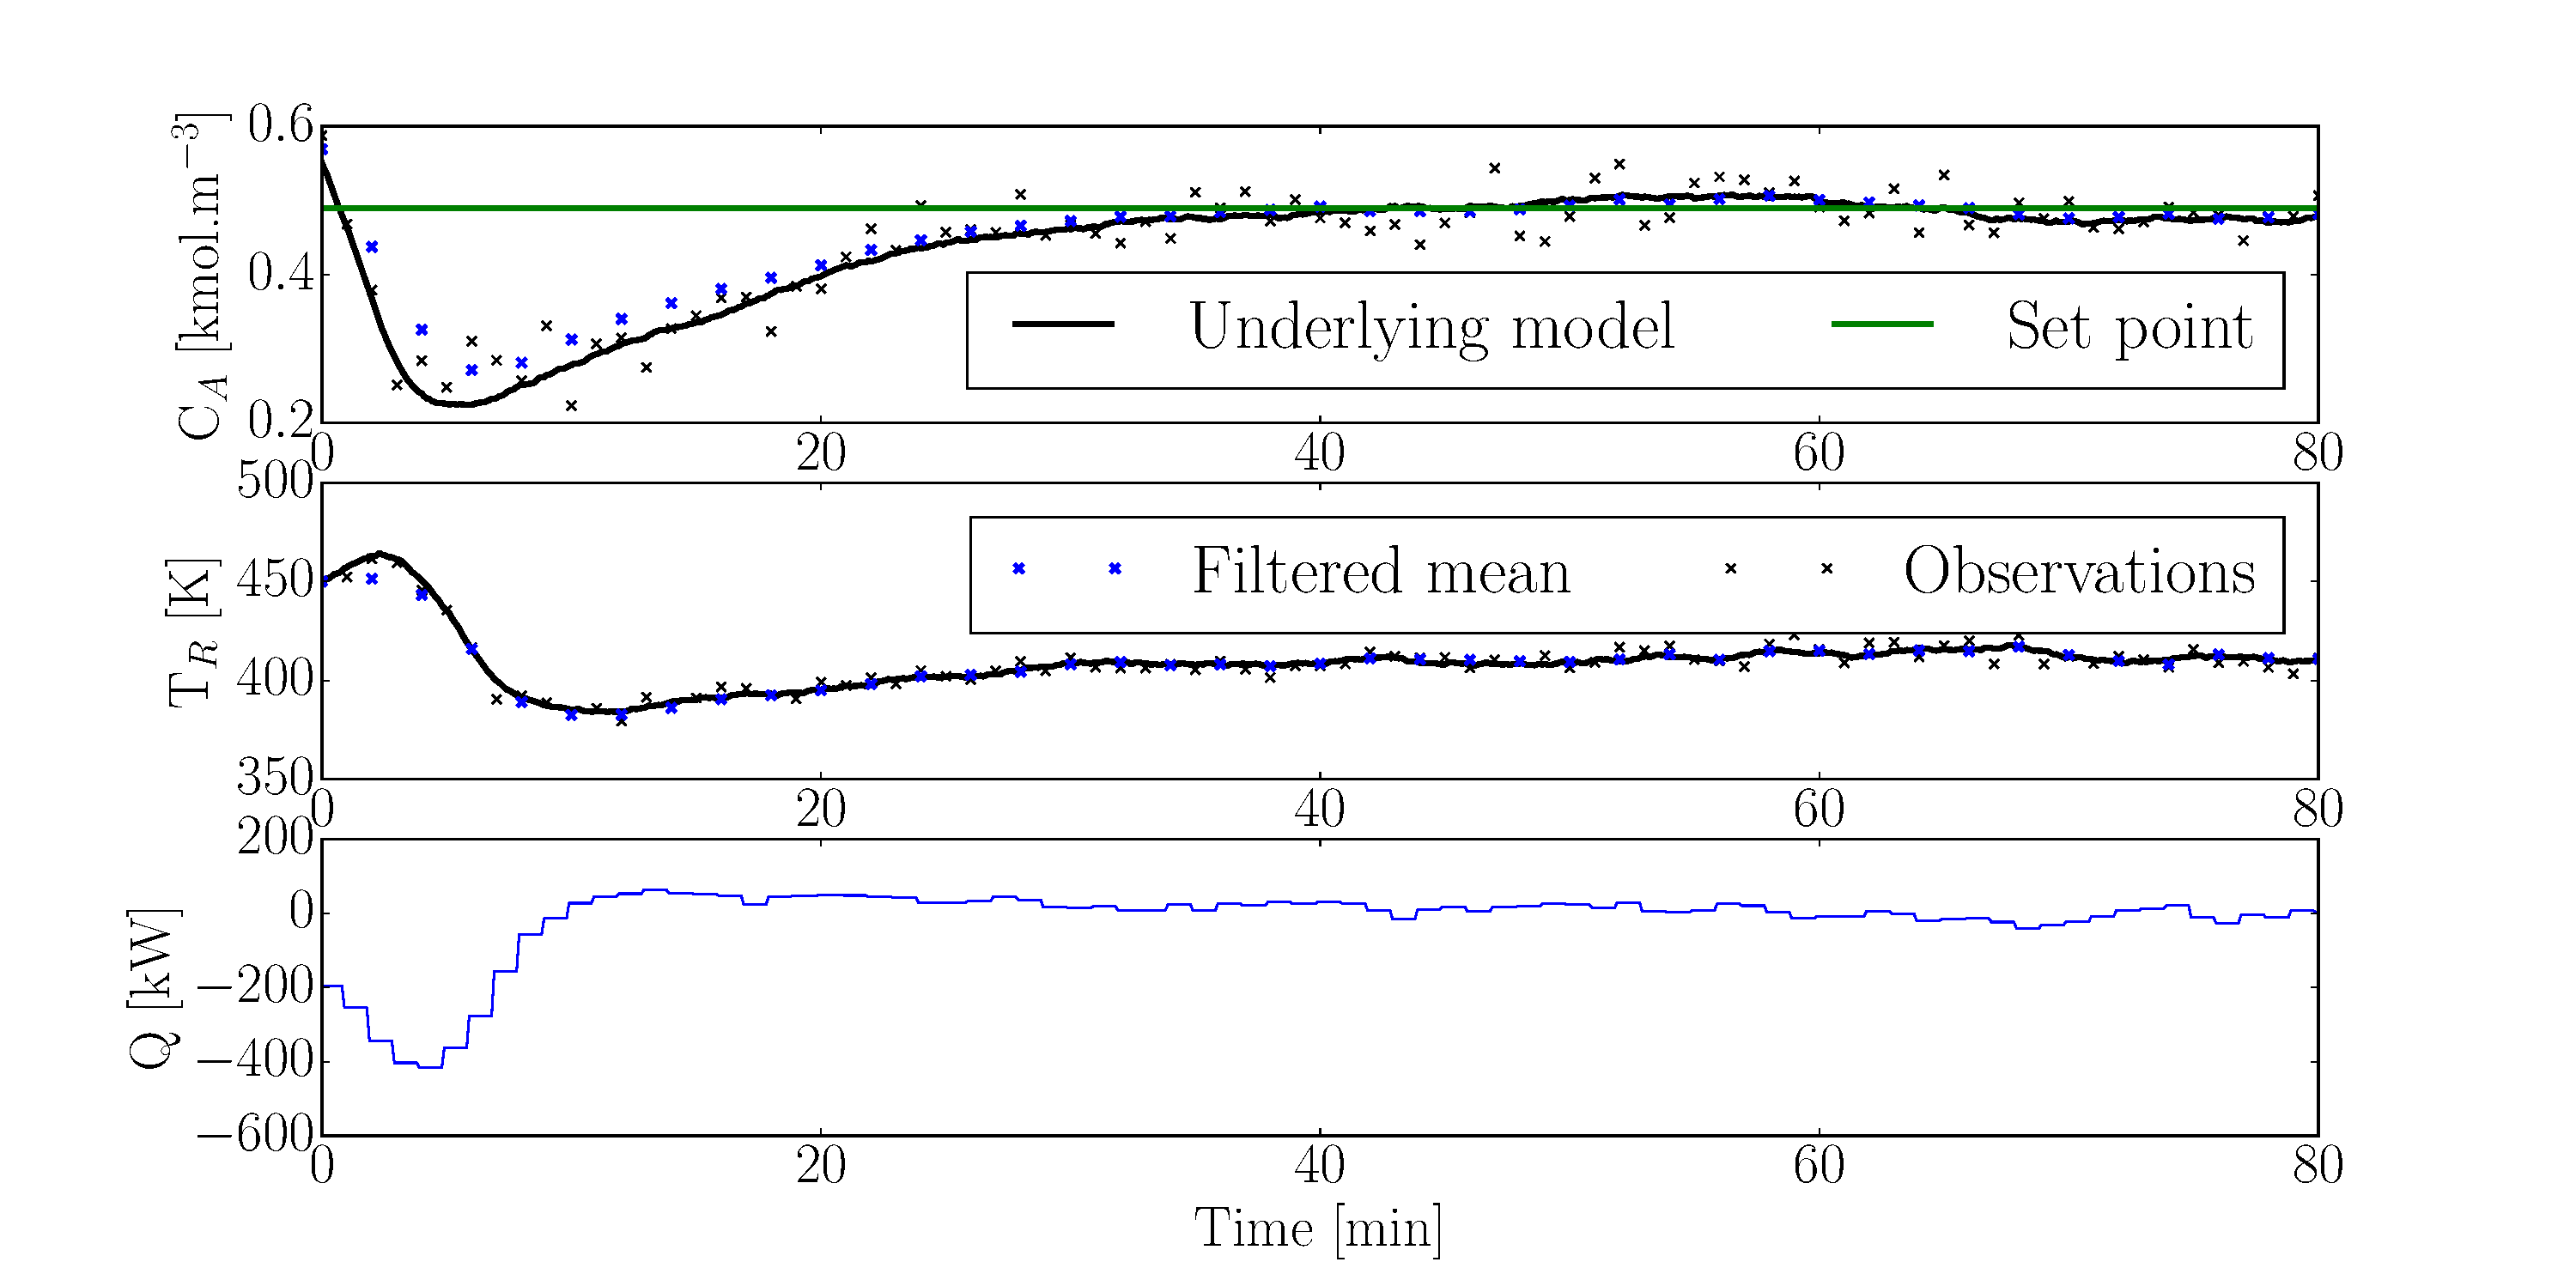
\includegraphics[width=\textwidth]{nonlin_mod_lqg.pdf}
\caption{LQG regulator tracking with initial condition (0.55, 450) and measuring both states.}
\label{fig_nonlin_lqg}
\end{figure}
The average energy usage and concentration error was 50.88 kW and 11.66\% respectively over the 80 min simulation time. Comparing Figures \ref{fig_lin_mod_lqg} and \ref{fig_nonlin_lqg} we see that the maximum absolute input energy is much greater with the non-linear underlying dynamics. This is not unexpected because the controller in both cases is linear: one expects the plant-model mismatch to have a detrimental effect on control.

In Chapter \ref{sec_lin_sys_cont} we had a linear underlying model and an almost linear controller. Figure \ref{fig_lin_mod_kl} also demonstrated that the posterior state distributions were approximately Gaussian. Thus there was no reason to use non-linear inference algorithms like the particle filter introduced in Chapter \ref{sec_inf_nonlin_mods}. However, in this chapter we are using a non-linear underlying model and it might be advantageous to use a more sophisticated inference tool. We investigate using both a Kalman filter and a particle filter for inference. In the setting of the particle filter we approximate the samples as Gaussian and use that for control.

As before we first investigate the deterministic MPC. The control problem is shown in (\ref{eq_mpc_constrained_det2}). Note that the constraints are different due to the expected extra difficulty introduced by the non-linear underlying model. 
\begin{equation}
\begin{aligned}
&\underset{\mathbf{u}}{\text{min }} \frac{1}{2}\sum_{k=0}^{N-1} \left( \mu_k^TQ\mu_k + u_k^TRu_k \right) + \frac{1}{2}\mu_N^TP_f\mu_N \\
& \text{subject to } \mu_{t+1}=A\mu_t + Bu_t \\
&\text{and } \begin{pmatrix}
10 \\ 1
\end{pmatrix}^T \mu_t + 406 \geq 0 ~\forall ~t=1,...,N\\
& \text{and } |u_t| \leq 330 ~\forall ~t=0,...,N-1\\
\end{aligned}
\label{eq_mpc_constrained_det2}
\end{equation}
In Figure \ref{fig_nonlin_mod_kf_mean_track} we see that the deterministic MPC using the Kalman filter for state inference does converge to the set point. The ability to naturally constrain the system is again highlighted in the input: as opposed to the peak $|420|$ kW required by the LQG controller the MPC manages to control the system while never requiring more than $|330|$ kW. 
\begin{figure}[H] 
\centering
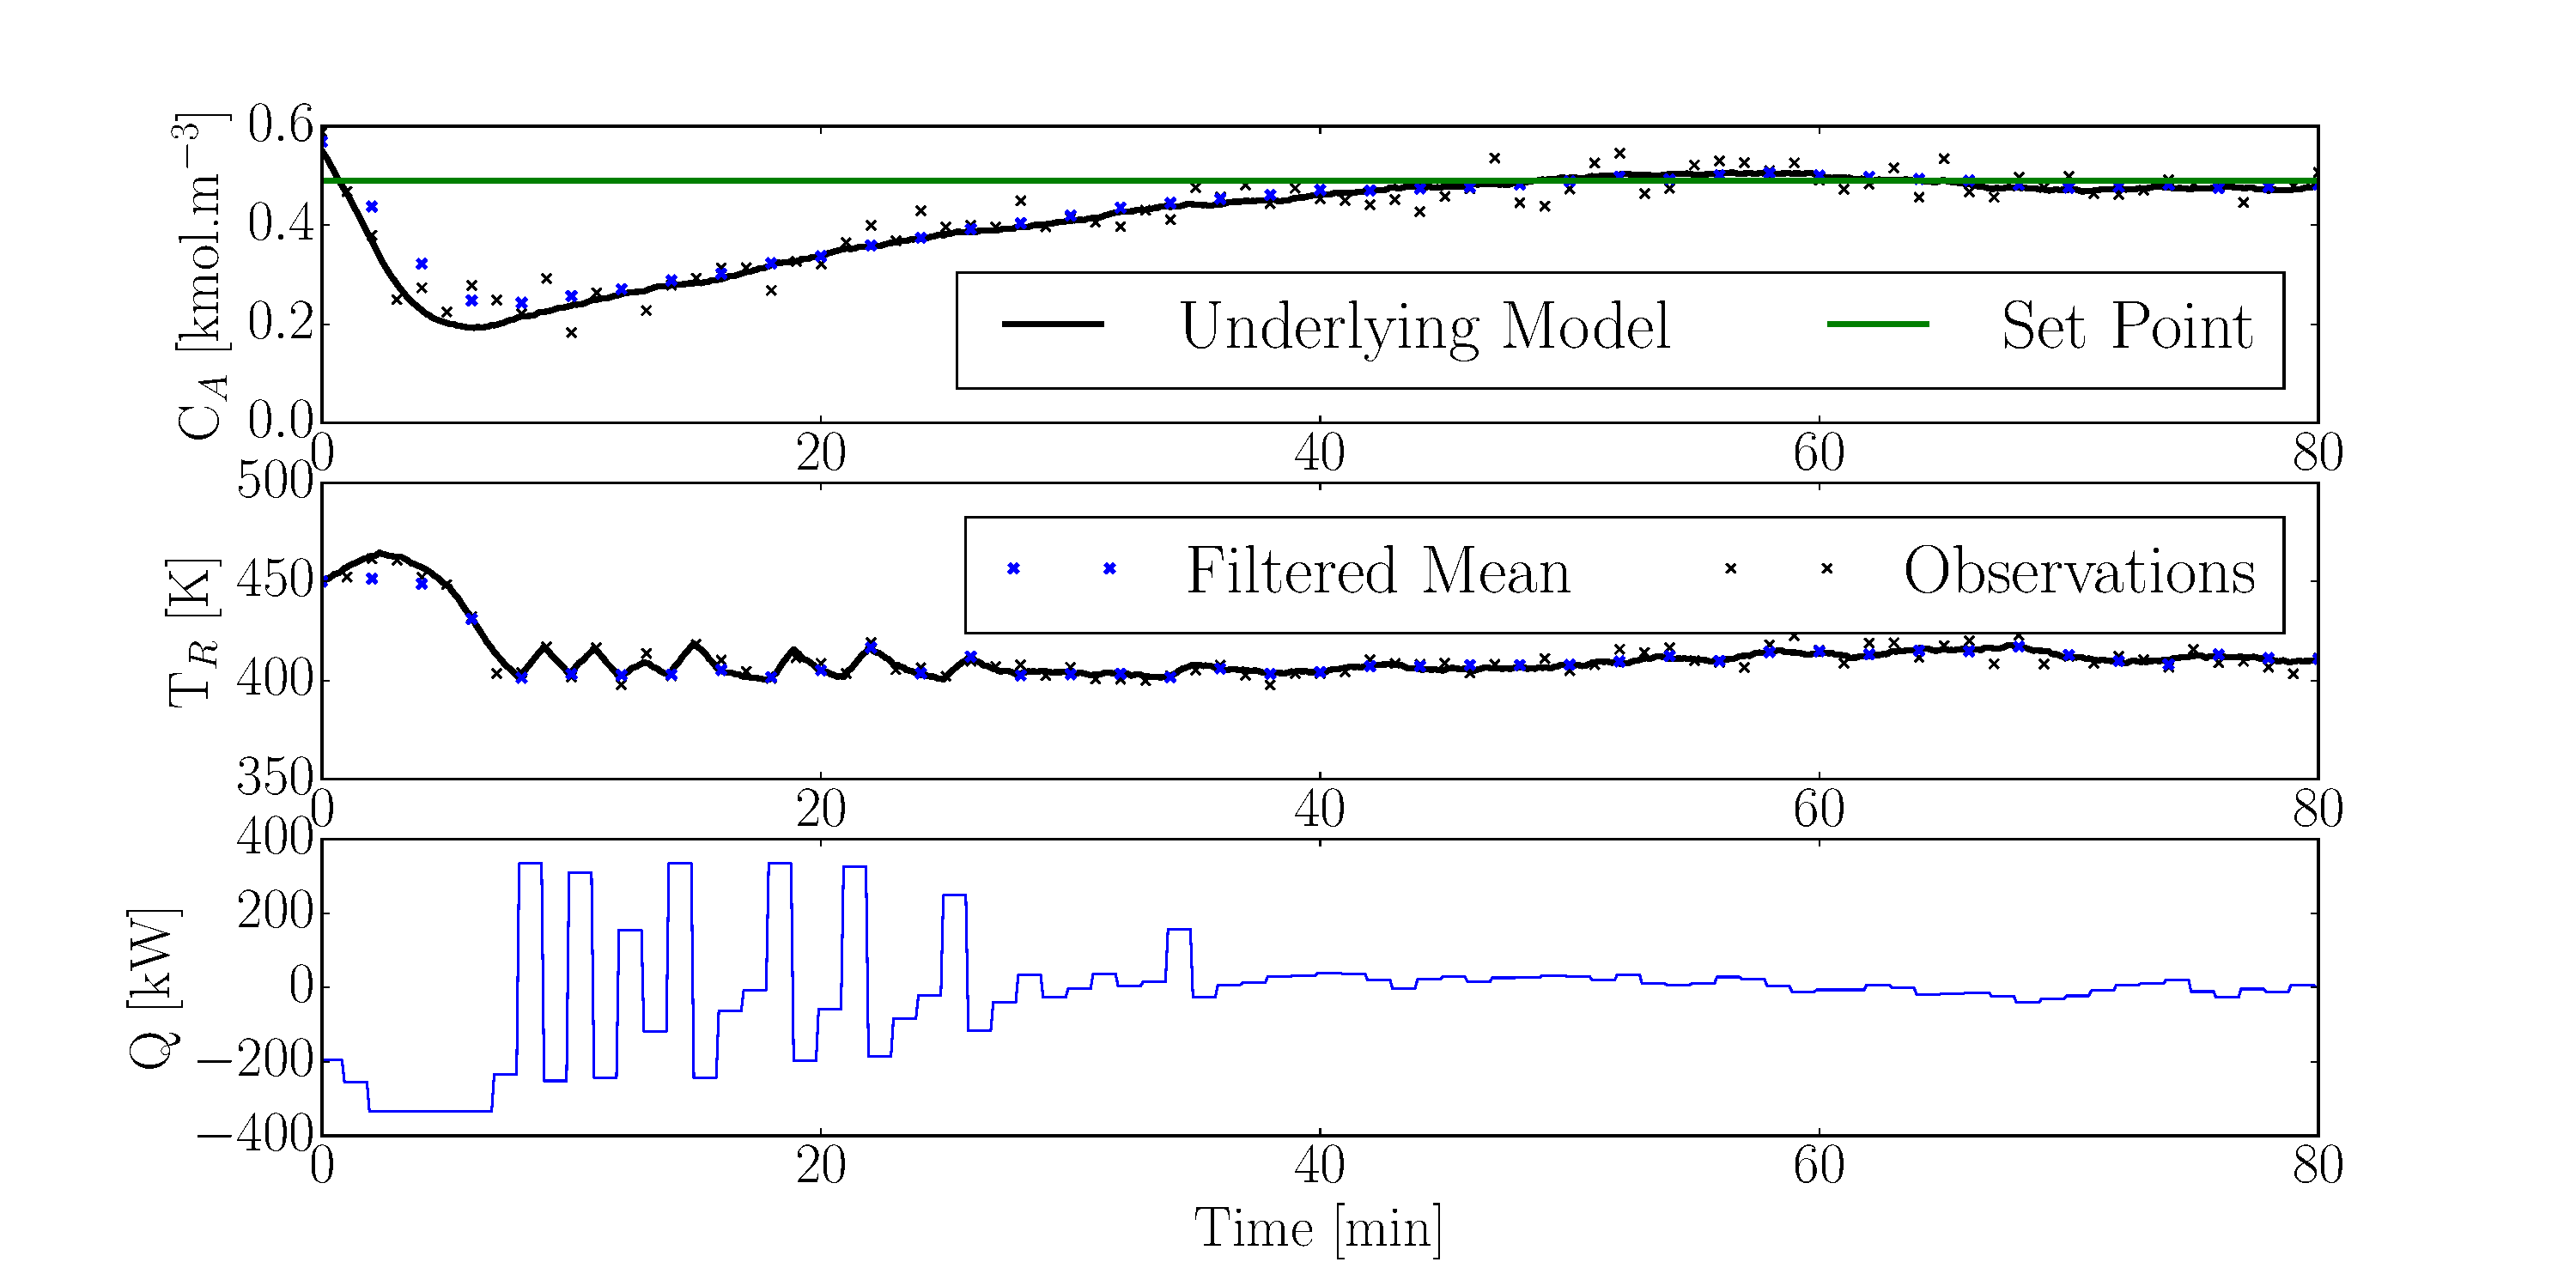
\includegraphics[width=\textwidth]{nonlin_mod_kf_mean_track.pdf}
\caption{Deterministic constrained MPC reference tracking with initial condition $(0.55, 450)$ and measuring both states. The Kalman filter is used for inference.}
\label{fig_nonlin_mod_kf_mean_track}
\end{figure} 
In Figure \ref{fig_nonlin_mod_kf_mean_ss} we see that the state constraint is violated just like Figure \ref{fig_lin_mod_kf_mean_ss}. We also see a somewhat unrealistic jagged state trajectory but this is just a numerical artefact. The average energy input and concentration error over the simulation run is 88.68 kW and 16.11\% respectively. The added constraints explain why the performance is degraded when compared to the LQG controller.
\begin{figure}[H] 
\centering
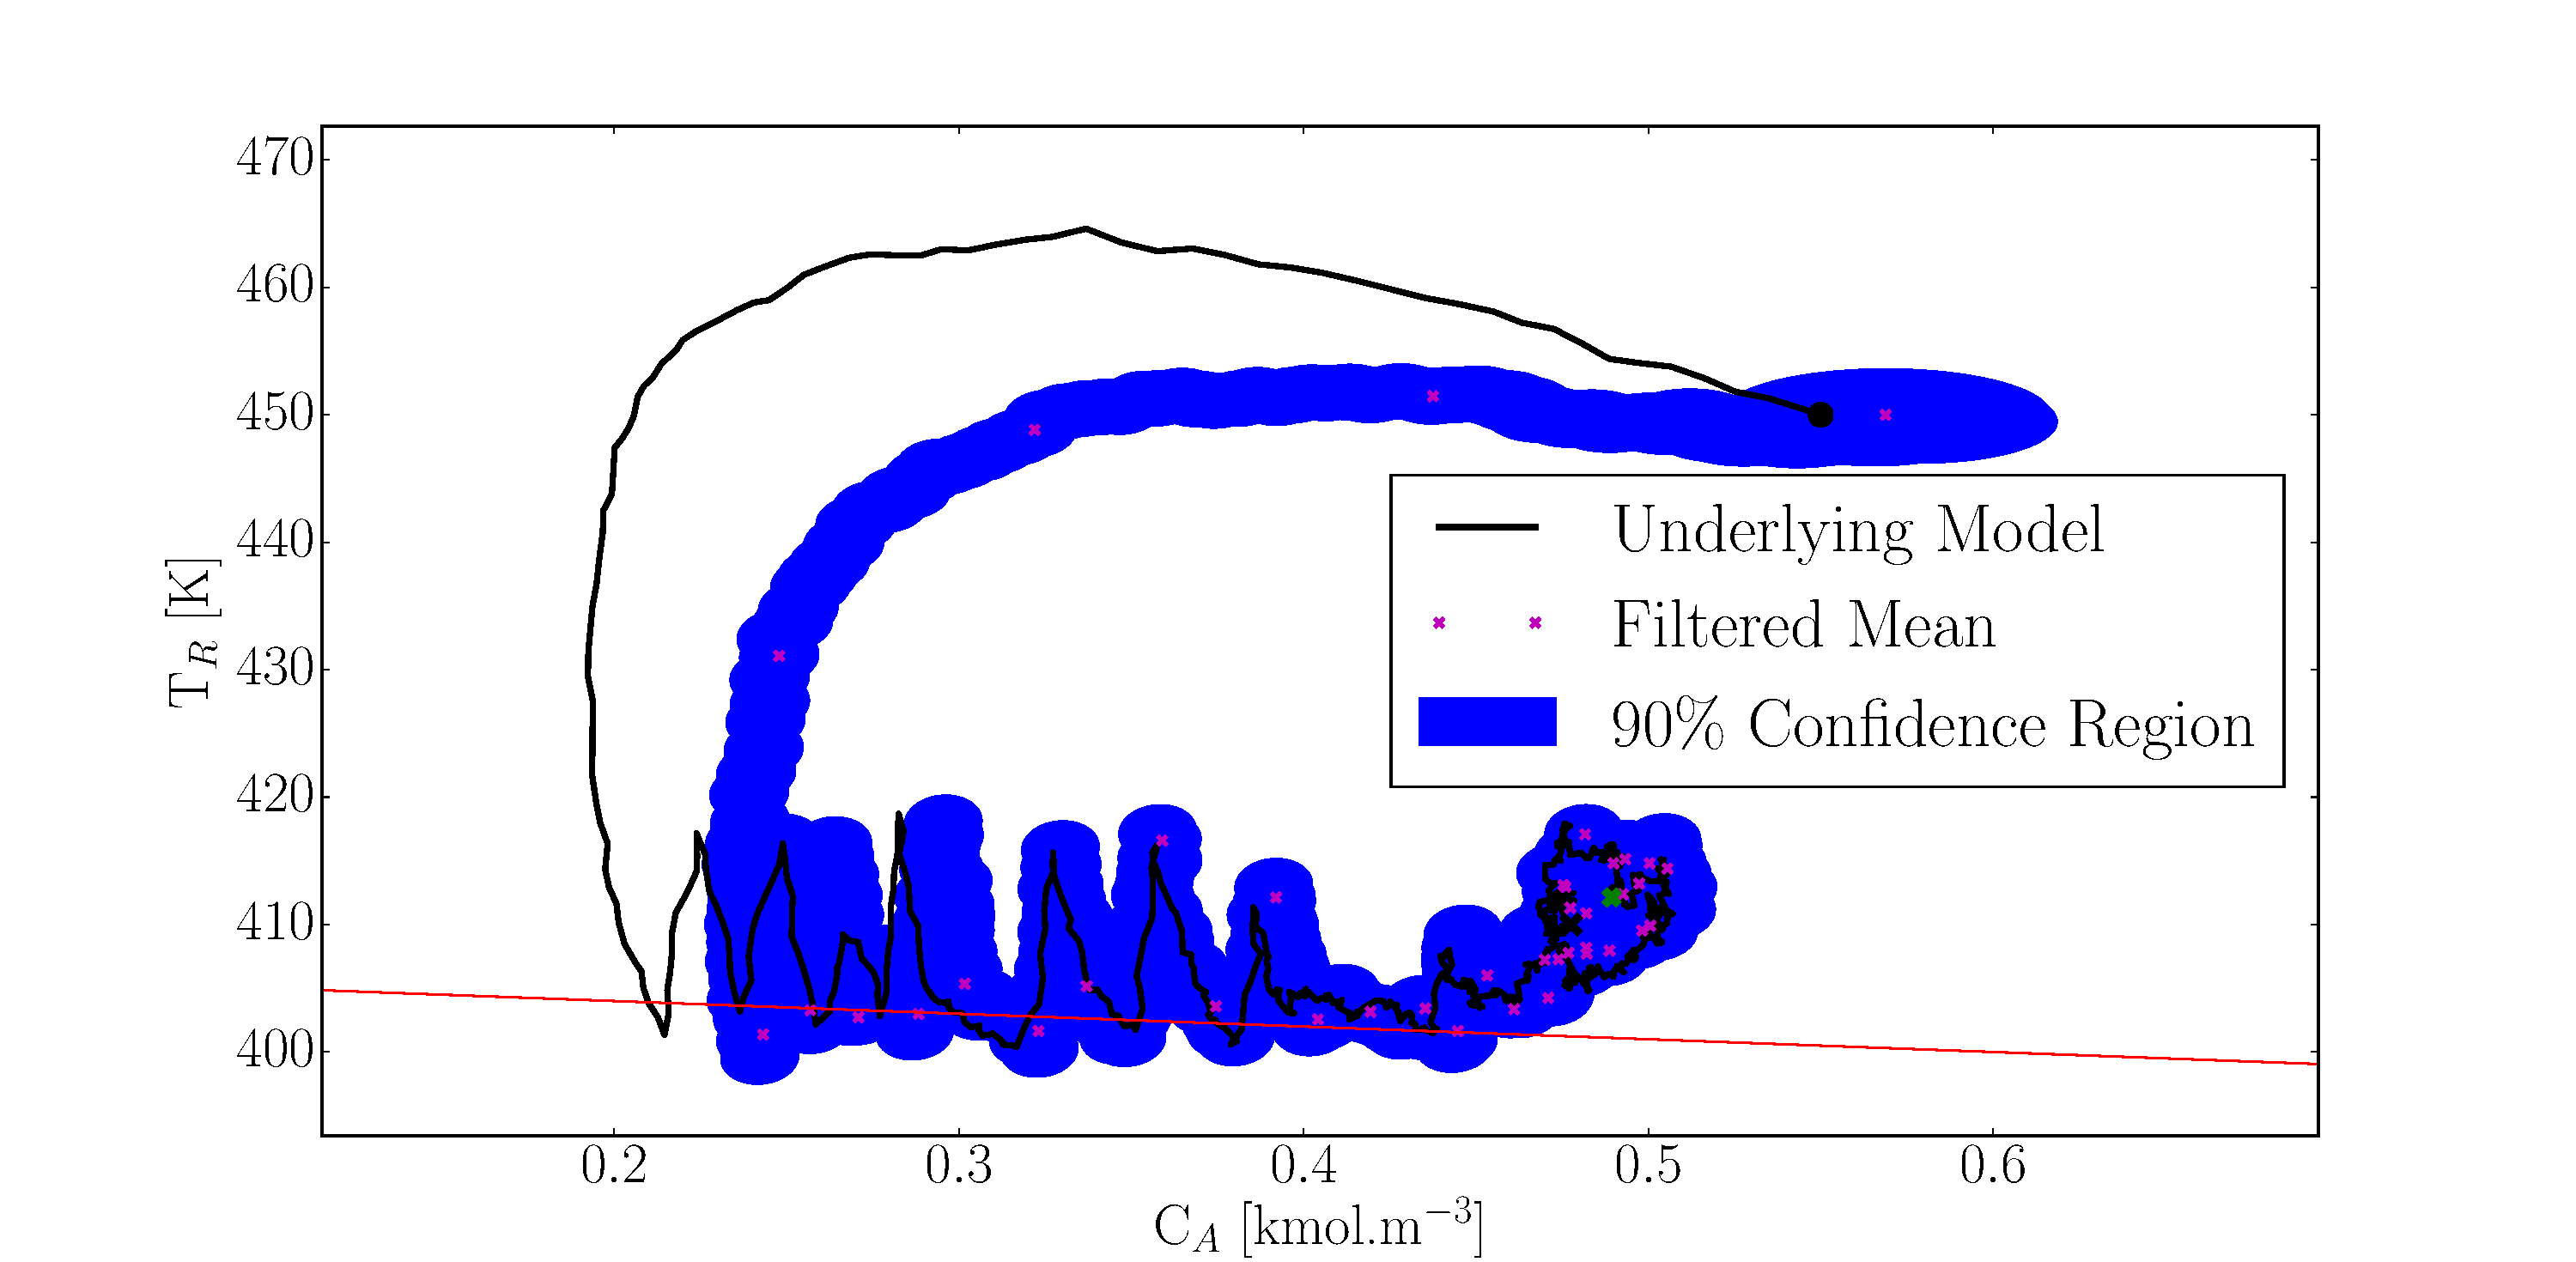
\includegraphics[width=\textwidth]{nonlin_mod_kf_mean_ss.pdf}
\caption{Deterministic constrained MPC state space trajectory with initial condition $(0.55, 450)$ and measuring both states. The Kalman filter is used for inference.}
\label{fig_nonlin_mod_kf_mean_ss}
\end{figure}
Since we are not using a chance constrained MPC the state constraint violation is not surprising in Figure \ref{fig_nonlin_mod_kf_mean_ss}. However, a more significant issue is the inability of the Kalman filter to accurately track the states throughout the simulation (the underlying system briefly diverges from the state estimates). This can be significantly problematic if a constraint existed in the left hand side of the state space: the controller wouldn't know that it was violating the constraint because the state estimate is poor. This behaviour is caused by the linear model used by the Kalman filter. The state trajectory moves away from the region close to the linearisation point and thus, as explained in Chapter \ref{sec_inf_lin_mods}, the state estimate becomes poor.

We can remedy this situation by using a more sophisticated inference algorithm. In Figure \ref{fig_nonlin_mod_pf_mean_track} we see the deterministic MPC using a particle filter with 200 particles for inference. 
\begin{figure}[H] 
\centering
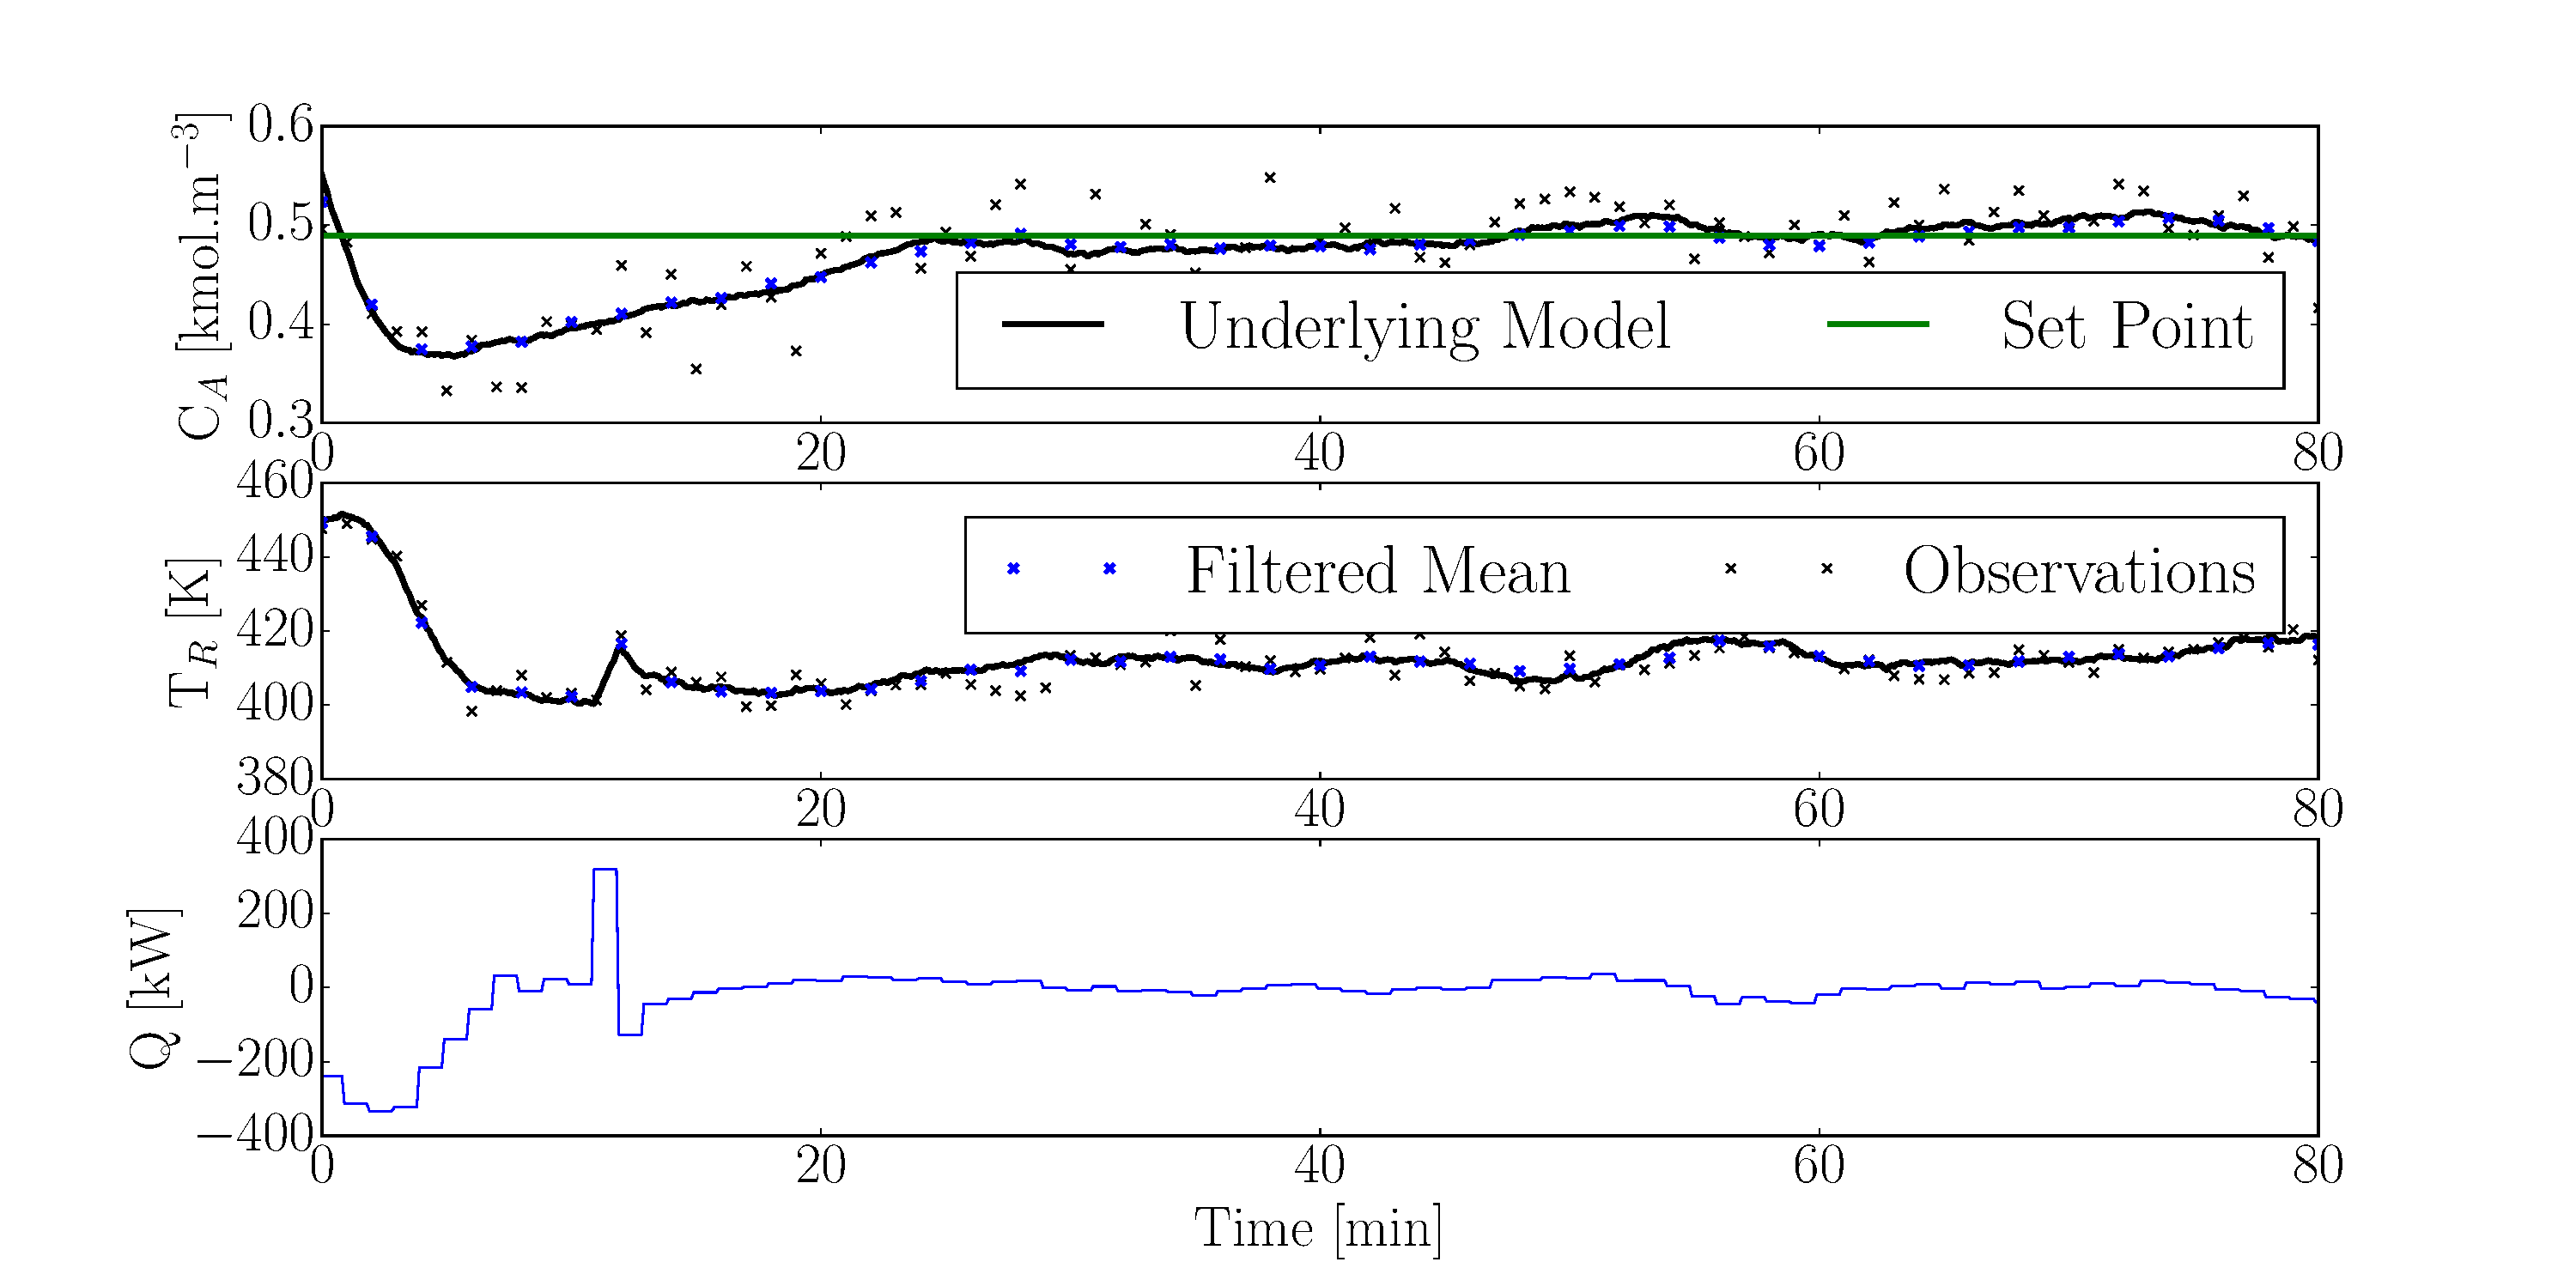
\includegraphics[width=\textwidth]{nonlin_mod_pf_mean_track.pdf}
\caption{Deterministic constrained MPC reference tracking with initial condition $(0.55, 450)$ and measuring both states. A particle filter with 200 particles is used for inference.}
\label{fig_nonlin_mod_pf_mean_track}
\end{figure} 
The average energy input and concentration error is 38.83 kW and 5.81\% respectively. This is a vast improvement over the same controller where the Kalman filter was used for inference. The benefit of accurate state estimation is apparent here and also in Figure \ref{fig_nonlin_mod_pf_mean_ss}.
\begin{figure}[H] 
\centering
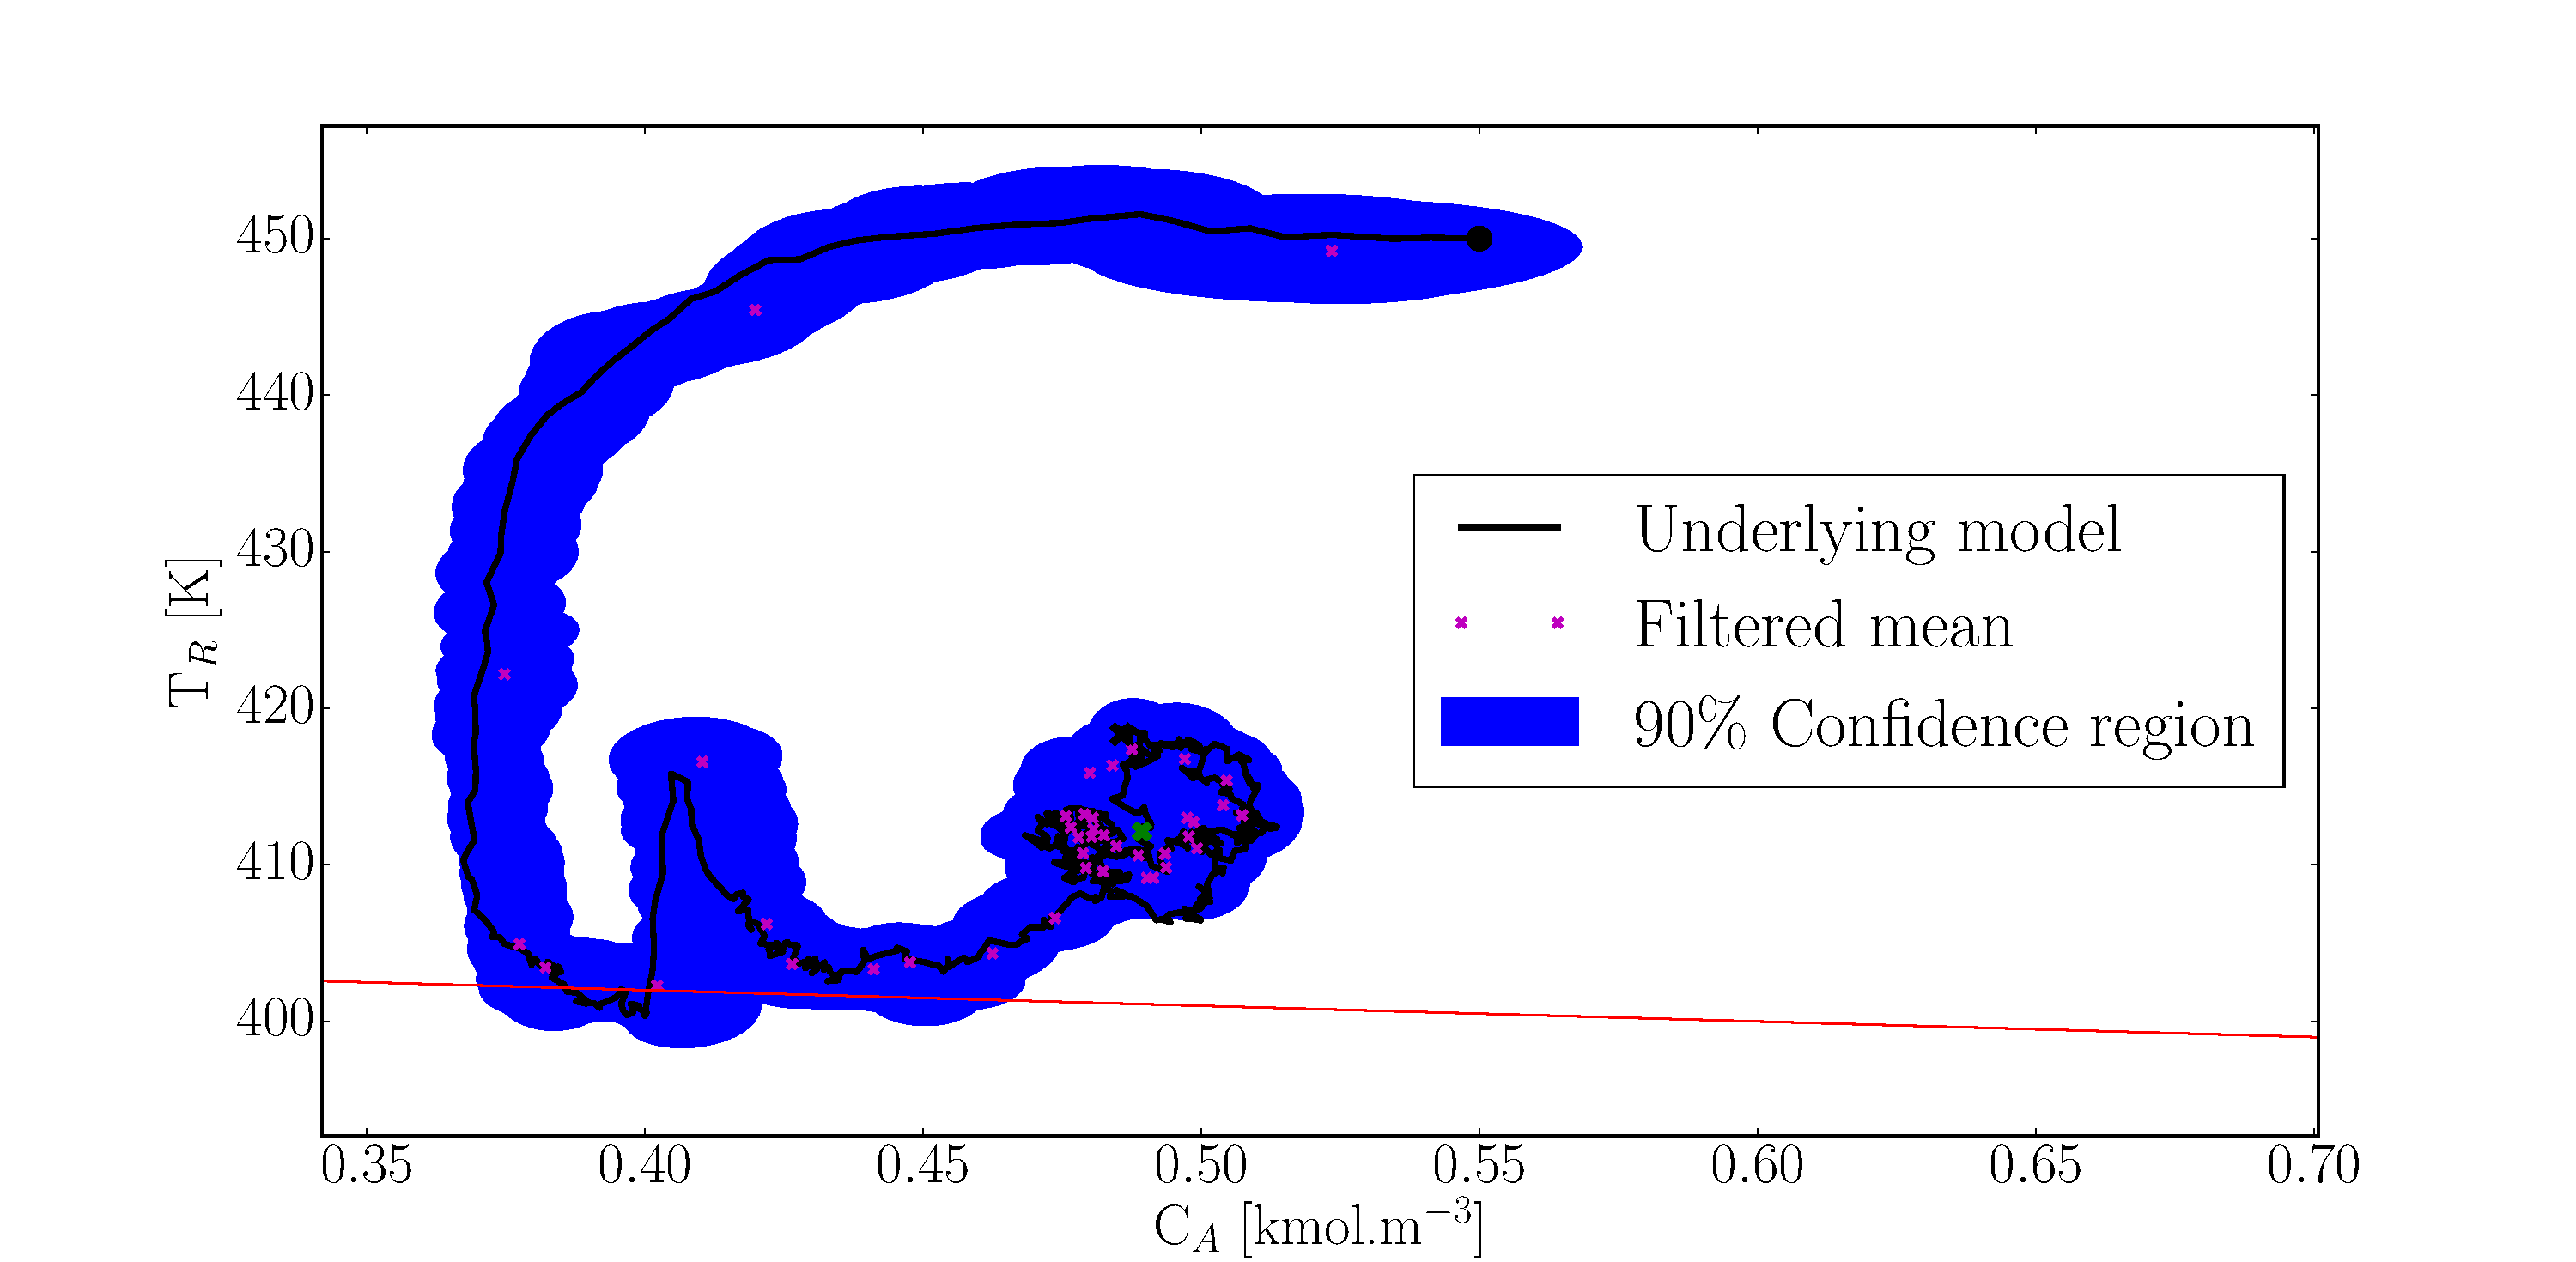
\includegraphics[width=\textwidth]{nonlin_mod_pf_mean_ss.pdf}
\caption{Deterministic constrained MPC state space trajectory with initial condition $(0.55, 450)$ and measuring both states. A particle filter with 200 particles is used for inference.}
\label{fig_nonlin_mod_pf_mean_ss}
\end{figure}
In Figure \ref{fig_nonlin_mod_kf_mean_ss} we saw significant estimation deviation from the true underlying state, while in Figure \ref{fig_nonlin_mod_pf_mean_ss} the deviation is negligible. We still have that the state constraint is violated but this is due to the stochastic nature of the underlying system. It is clear that the particle filter MPC combination is superior to the Kalman filter MPC combination in this case. However, the benefit of using the particle filter should be weighed against the cost of the algorithm especially in higher dimensions where it is known that the particle filter does not perform well (recall the discussion following Figure \ref{fig_pf_kf_phase2}).

Now we introduce the chance constrained MPC in (\ref{eq_mpc_nonlin_mod_cons}). Note that the constraints are different than (\ref{eq_mpc_linmod_kf_cons}) for the same reason as (\ref{eq_mpc_constrained_det2}). We have $d^T = (10, 1)$ and $e=406$ as before. By consulting the Chi Squared distribution table we set $k^2 = 4.6052$ which corresponds to the chance constraint $\text{Pr}(d^Tx_t + e \geq 0) \geq 90\% ~\forall ~t=1,...,N$ exactly as in the previous chapter.
\begin{equation}
\begin{aligned}
&\underset{\mathbf{u}}{\text{min }} \frac{1}{2}\sum_{k=0}^{N-1} \left( \mu_k^TQ\mu_k + u_k^TRu_k \right) + \frac{1}{2}\mu_N^TP_f\mu_N + \frac{1}{2}\sum_{k=0}^N \text{tr}(Q\Sigma_k) \\
& \text{subject to } \mu_{t+1}=A\mu_t + Bu_t \\
& \text{and } \Sigma_{t+1} = W+A\Sigma_t A^T \\
& \text{and } d^T\mu_t + e \geq k\sqrt{d^T \Sigma_t d} ~\forall ~t=1,...,N\\
& \text{and } |u_t| \leq 330 ~\forall ~t=0,...,N-1\\
\end{aligned}
\label{eq_mpc_nonlin_mod_cons}
\end{equation}
As with the deterministic case we first investigate the system where a Kalman filter is used for inference. Figure \ref{fig_nonlin_mod_kf_var90_track} illustrates that the chance constrained system does indeed converge to the set point. The average energy input and concentration error is 80.75 kW and 14.12\%. The average energy usage and average concentration error is reduced compared to the deterministic system. 
\begin{figure}[H] 
\centering
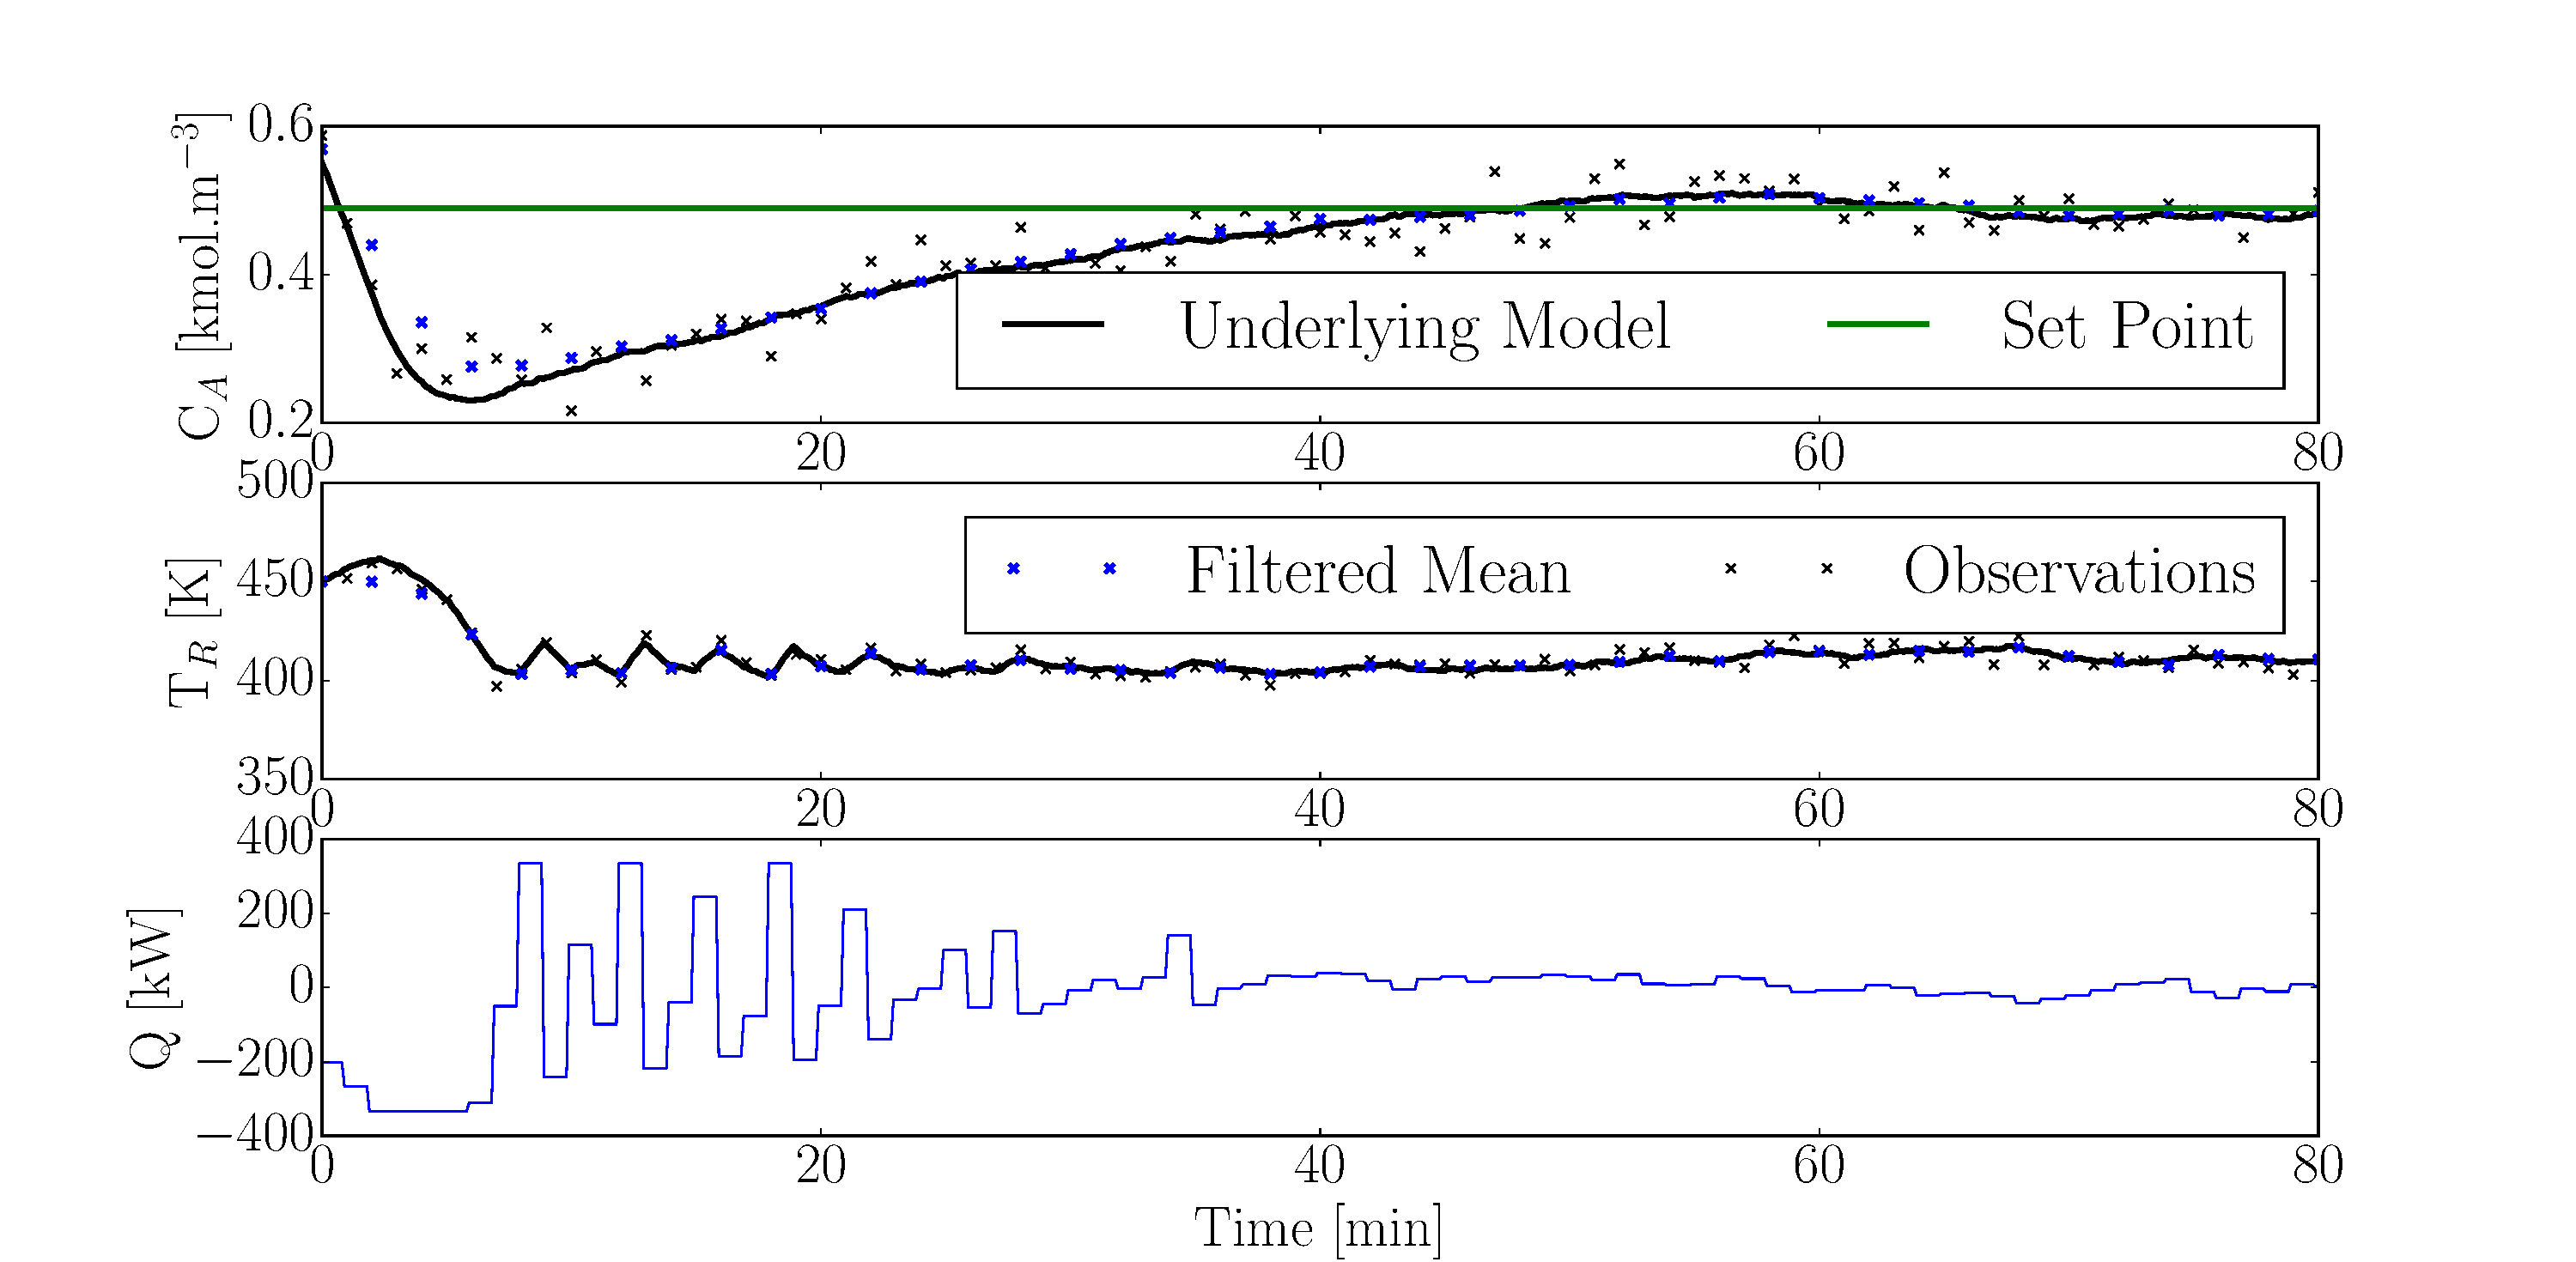
\includegraphics[width=\textwidth]{nonlin_mod_kf_var90_track.pdf}
\caption{Chance constrained MPC tracking with initial condition $(0.55, 450)$ and measuring both states. A Kalman filter is used for inference and the chance constraint is set at 90\%.}
\label{fig_nonlin_mod_kf_var90_track}
\end{figure}
The benefit of adding the chance constraint is apparent in Figure \ref{fig_nonlin_mod_kf_var90_ss}. It is clear that the constraint on the underlying state is not violated as much as in Figure \ref{fig_nonlin_mod_kf_mean_ss}. 
\begin{figure}[H] 
\centering
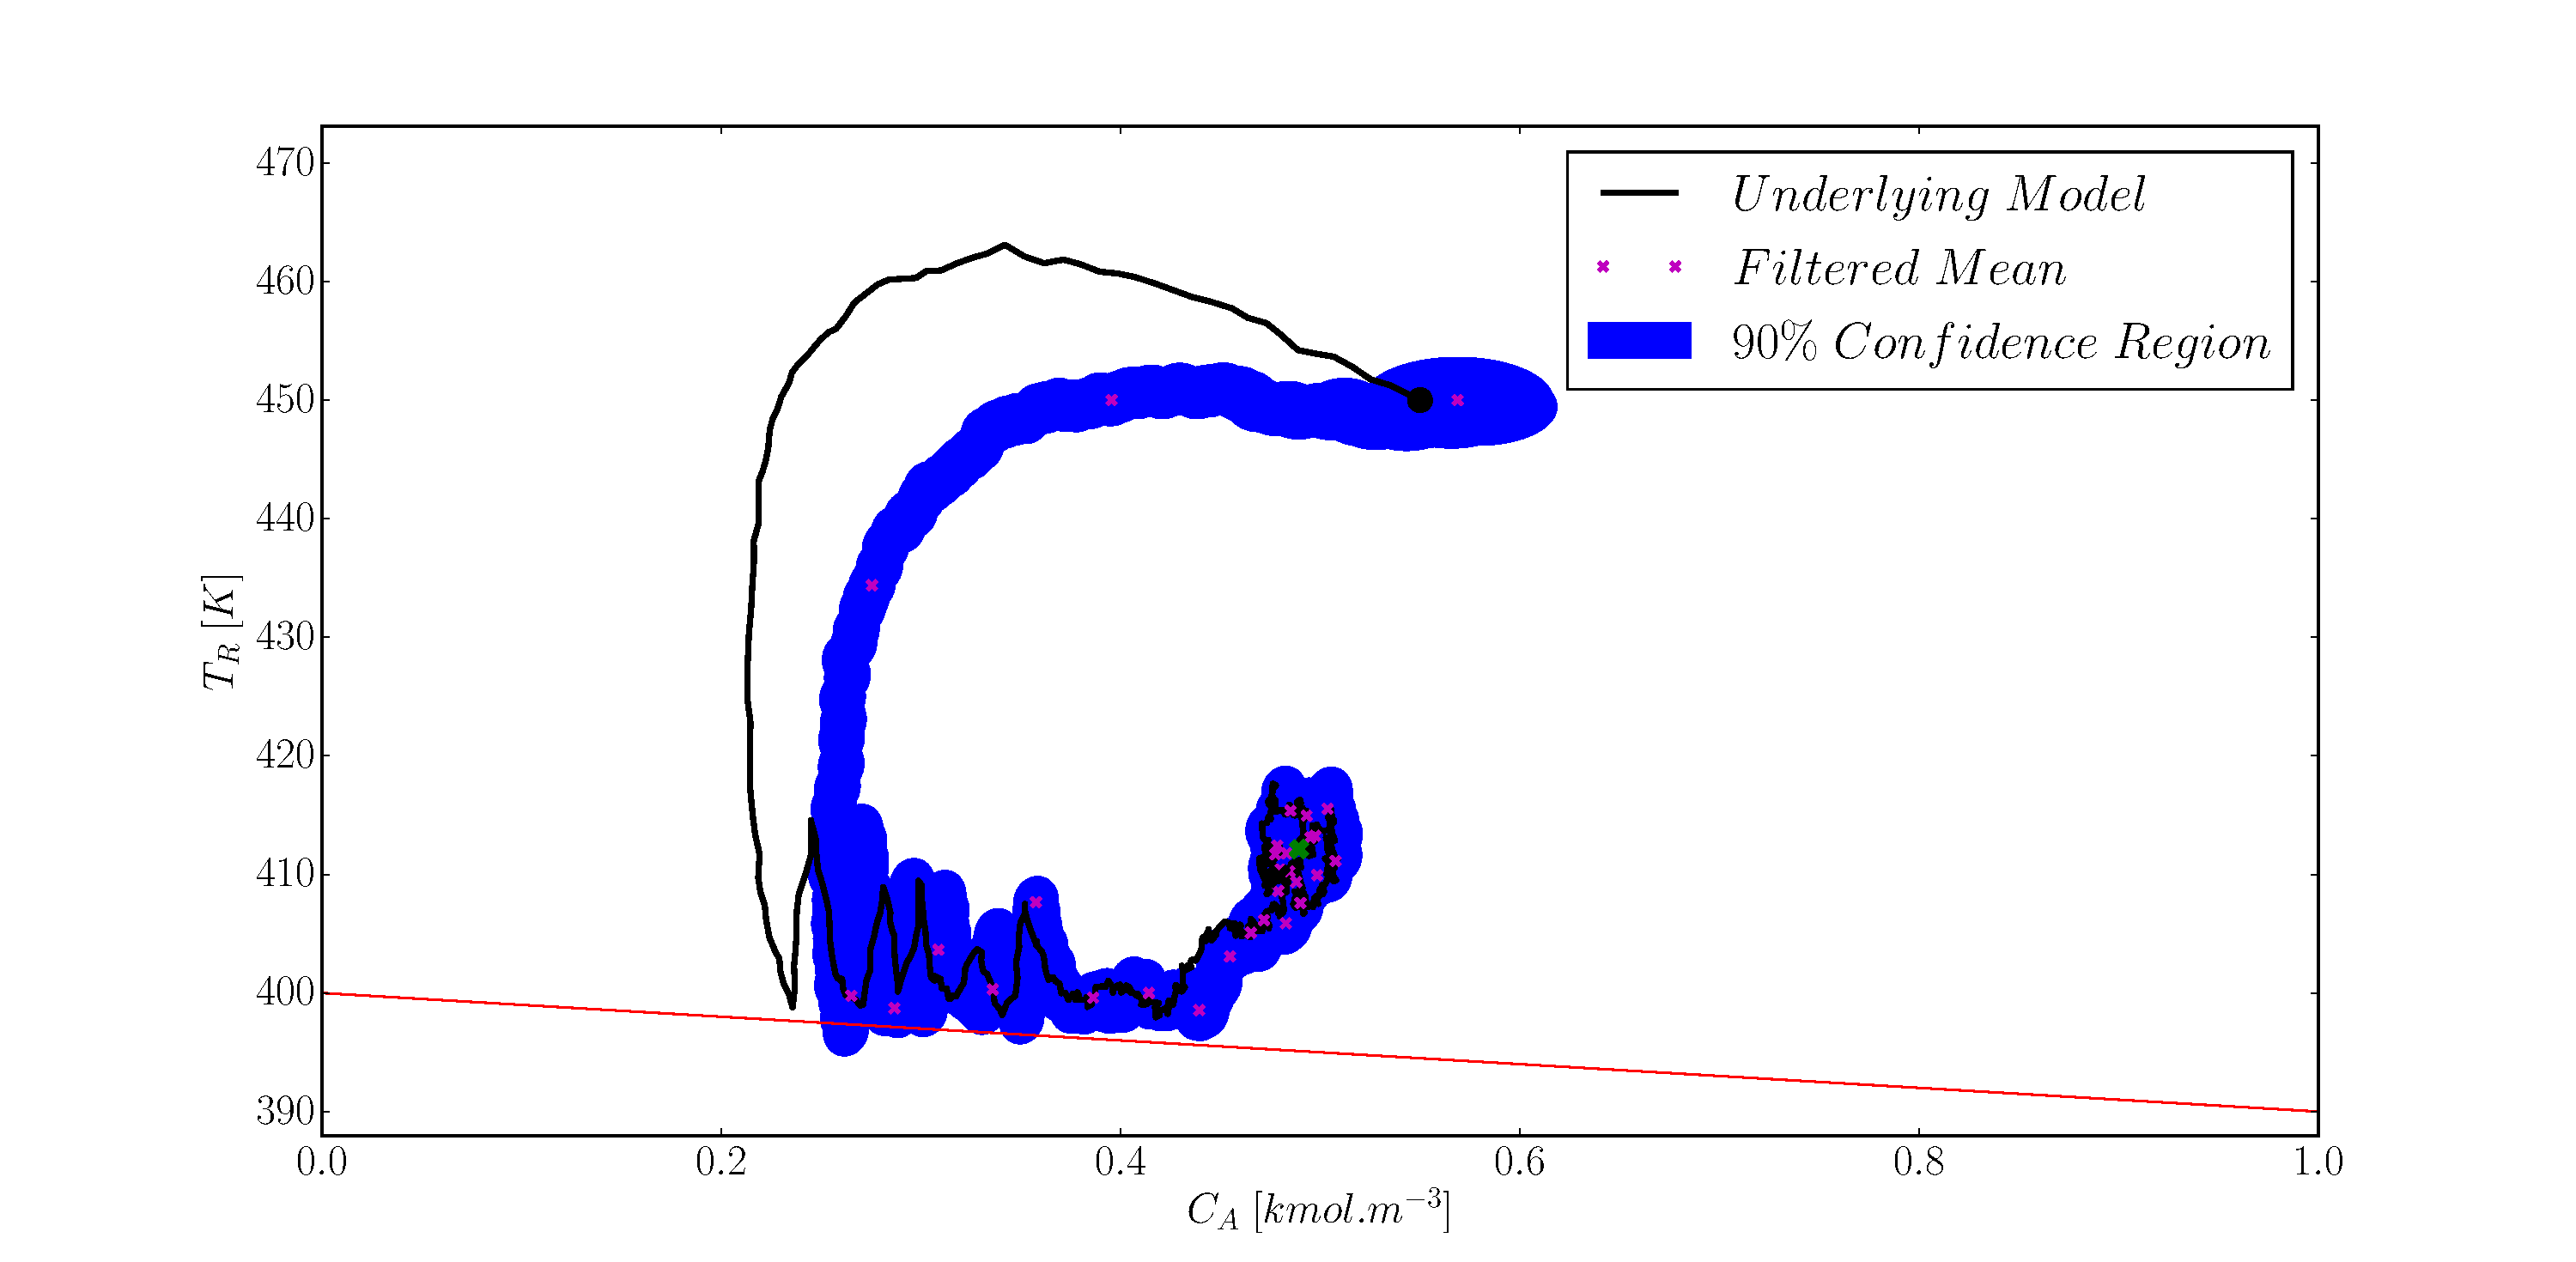
\includegraphics[width=\textwidth]{nonlin_mod_kf_var90_ss.pdf}
\caption{Chance constrained MPC state space trajectory with initial condition $(0.55, 450)$ and measuring both states. A Kalman filter is used for inference and the chance constraint is set at 90\%.}
\label{fig_nonlin_mod_kf_var90_ss}
\end{figure}
It is clear that the non-linearity of the underlying system makes stochastic control difficult. By increasing $k^2=9.21$ which corresponds to changing the chance constraint such that $\text{Pr}(d^Tx_t + e \geq 0) \geq 99\% ~\forall ~t=1,...,N$ we hope to increase the minimum distance between the constraint and the underlying state.

Figure \ref{fig_nonlin_mod_kf_var99_track} shows the tracking of the modified system. The average energy input and average concentration error is 69.67 kW and 12.44\% respectively. It is quite interesting that the more conservative system performs better with regard to these to metrics than the less conservative system.
\begin{figure}[H] 
\centering
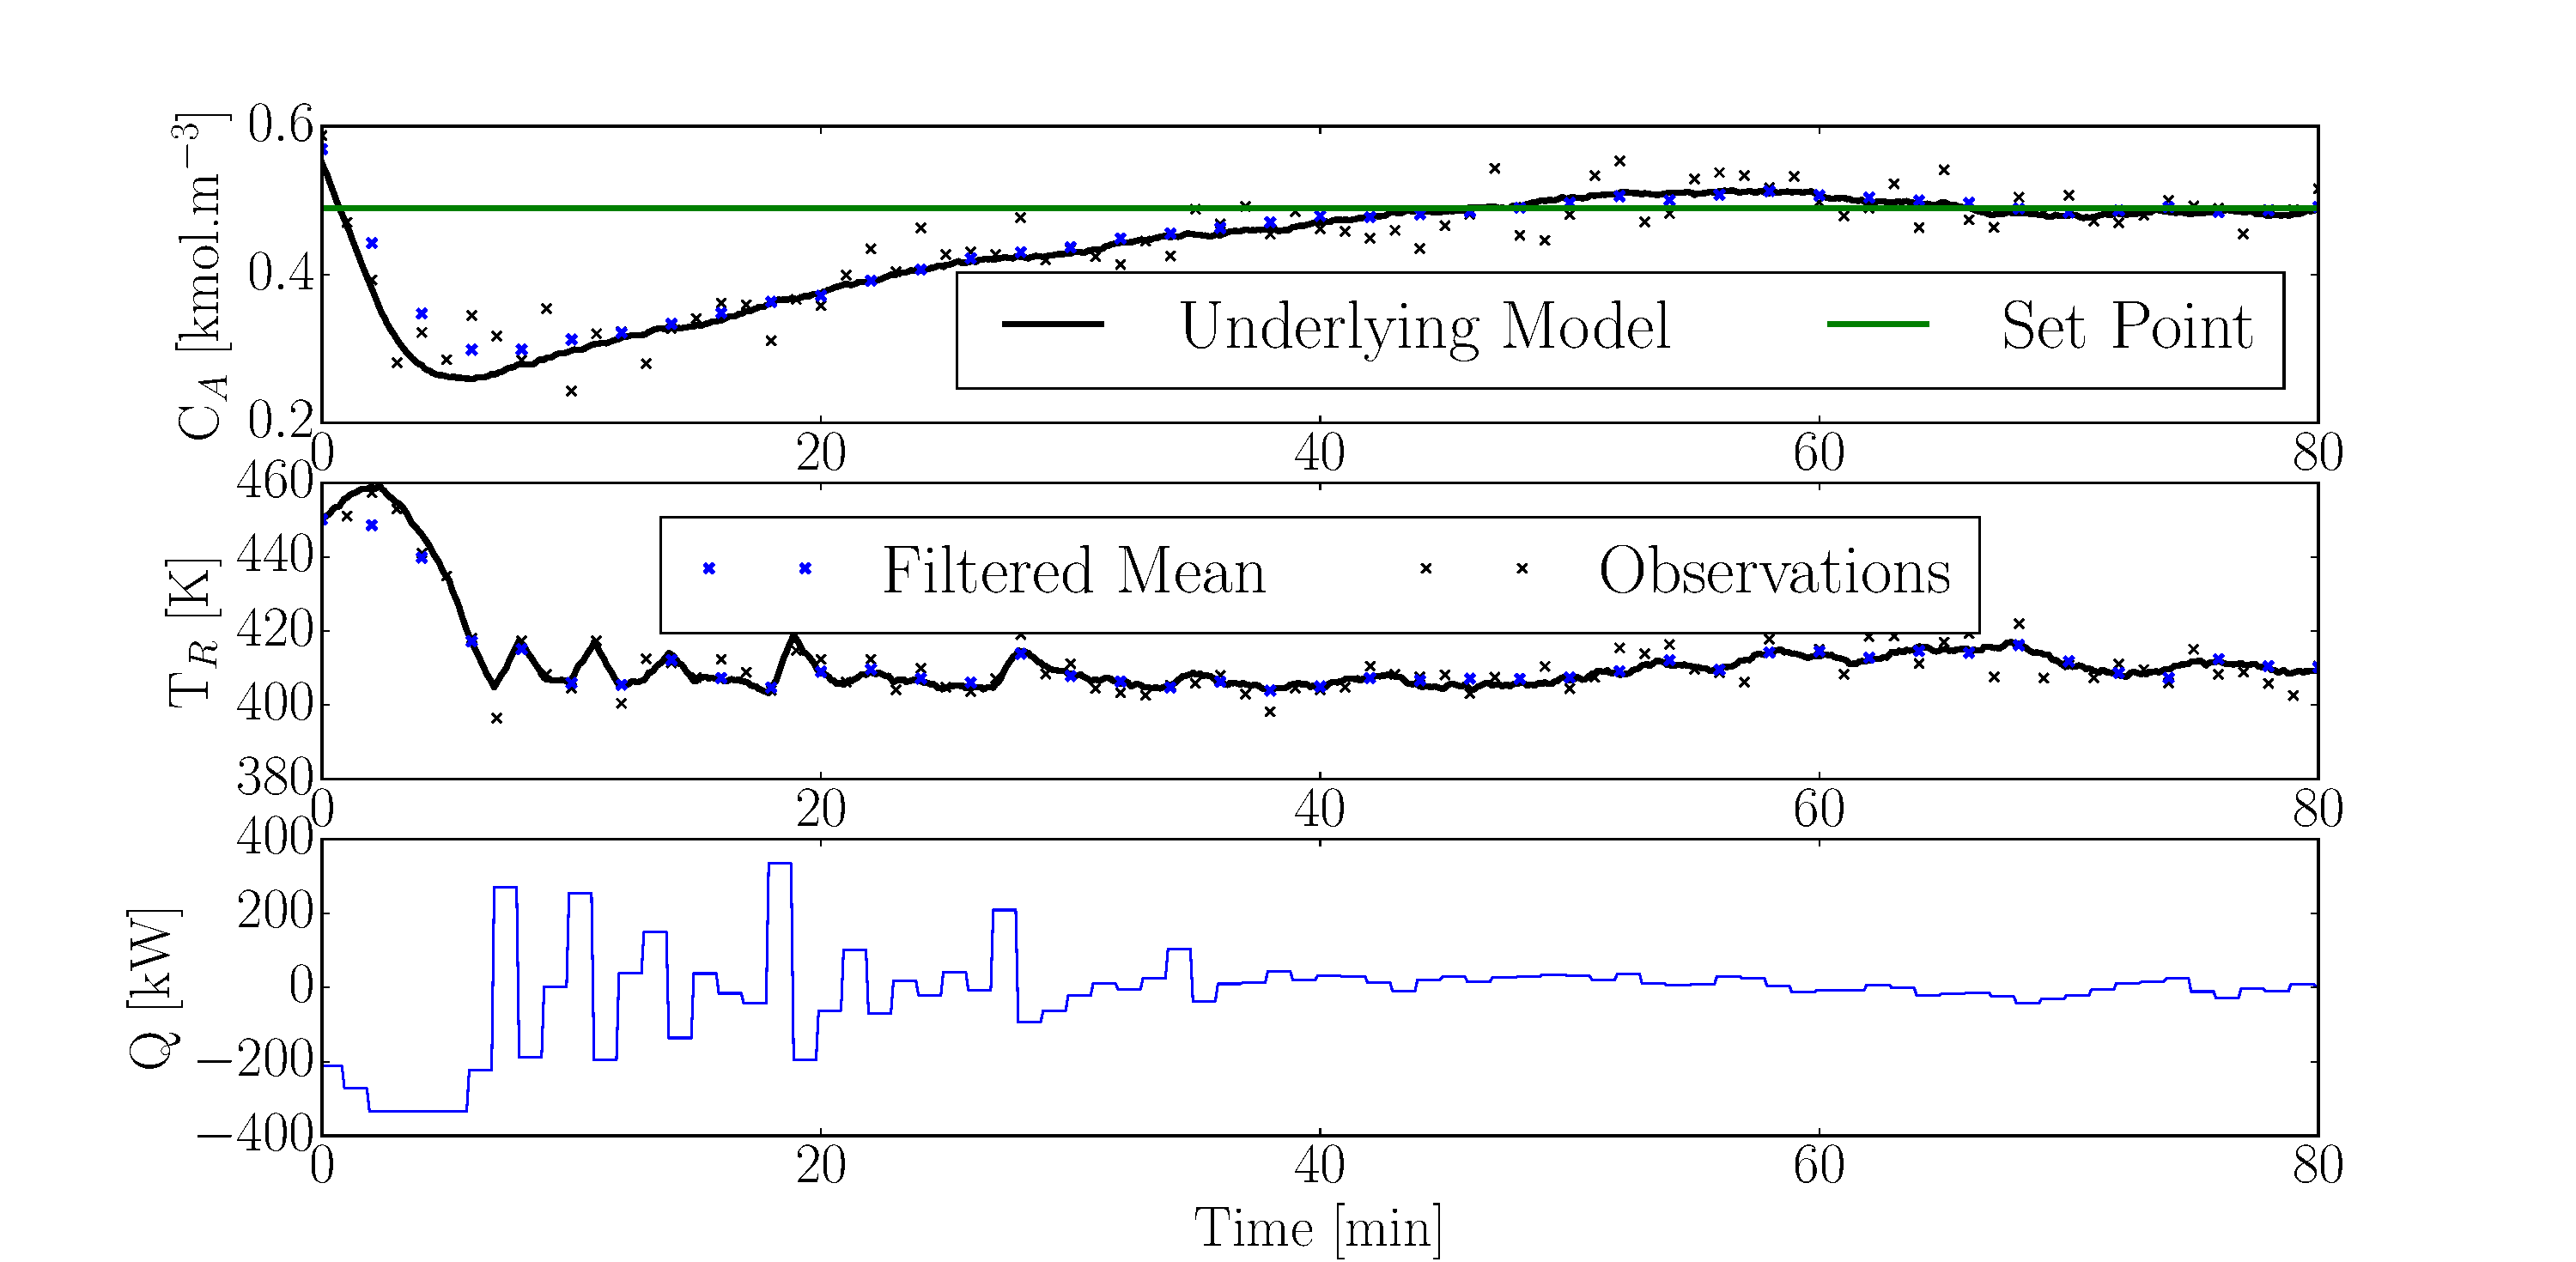
\includegraphics[width=\textwidth]{nonlin_mod_kf_var99_track.pdf}
\caption{Chance constrained MPC tracking with initial condition $(0.55, 450)$ and measuring both states. A Kalman filter is used for inference and the chance constraint is set at 99\%.}
\label{fig_nonlin_mod_kf_var99_track}
\end{figure}
In Figure \ref{fig_nonlin_mod_kf_var99_ss} we see that the margin of safety is increased although the confidence region still spills over the constraint. However, there is no constraint violation in this case.
\begin{figure}[H] 
\centering
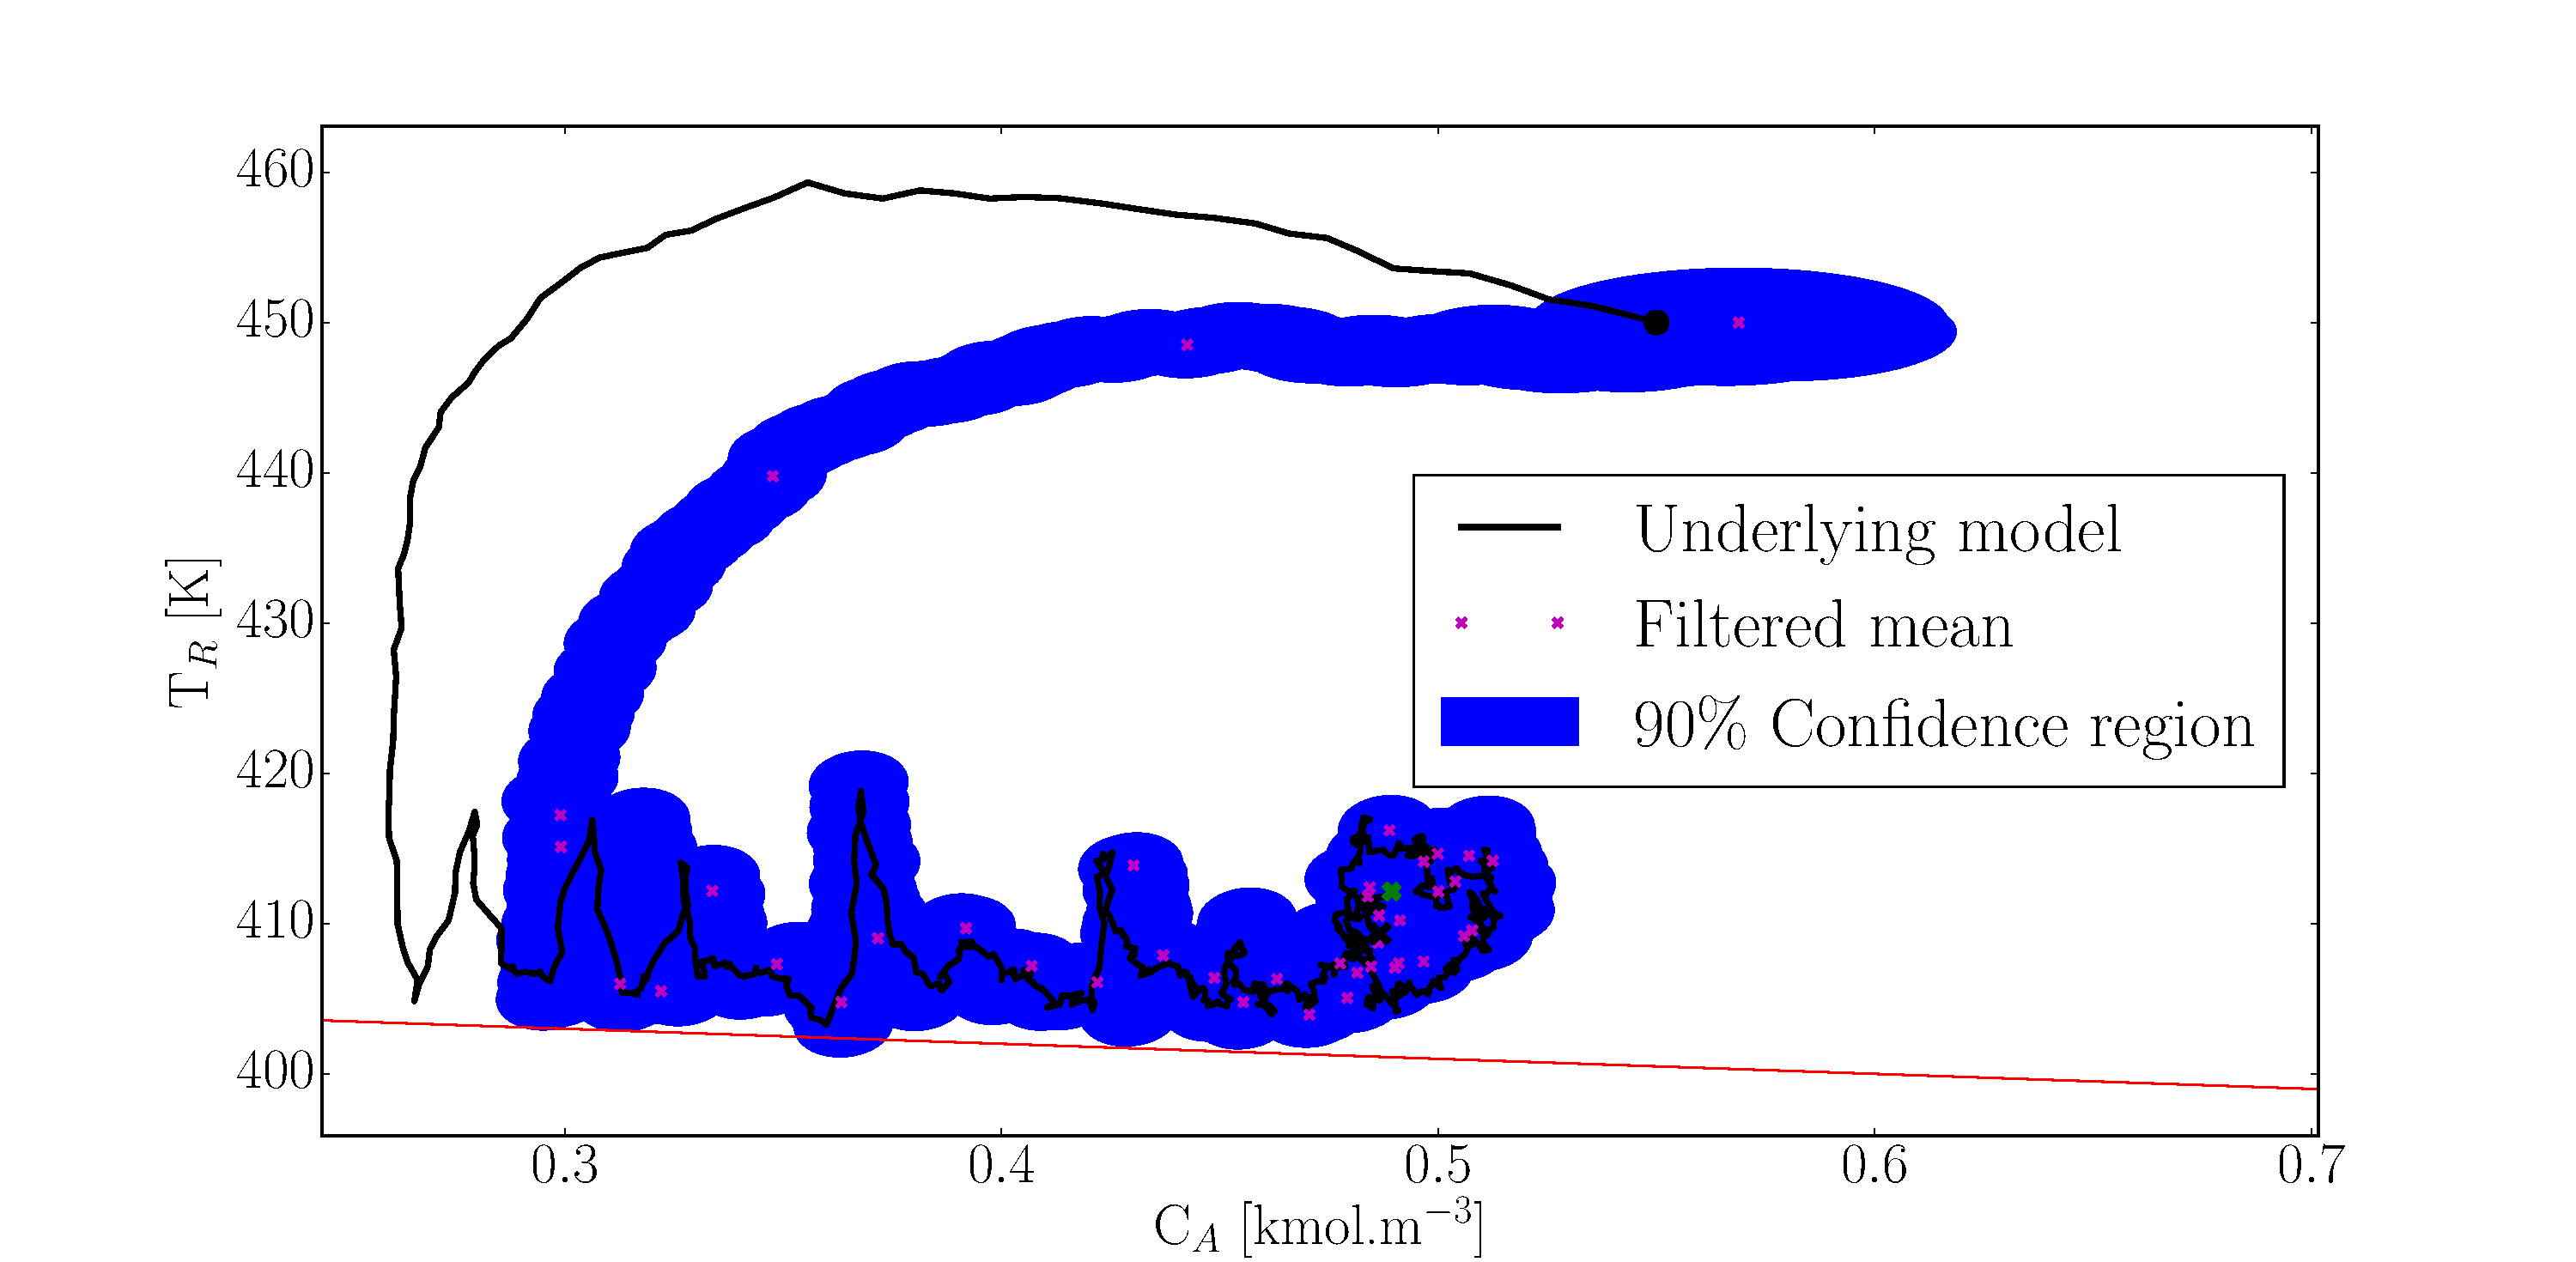
\includegraphics[width=\textwidth]{nonlin_mod_kf_var99_ss.pdf}
\caption{Chance constrained MPC state space trajectory with initial condition $(0.55, 450)$ and measuring both states. A Kalman filter is used for inference and the chance constraint is set at 99\%.}
\label{fig_nonlin_mod_kf_var99_ss}
\end{figure}
The ability of $k$ to increase or decrease the conservativeness of the constraint lends credibility to its value, if the system is non-normal, at the very least as an empirical measure to include stochastic robustness to the MPC in an efficient way.

Finally, Figure \ref{fig_lin_mod_kf_mc} illustrates the effect increasing $k^2$ (i.e. the threshold for the chance constraint) has on the system. Over 2000 simulations were used to illustrate that these tendencies hold not just for a specific realisation. 
\begin{figure}[H] 
\centering
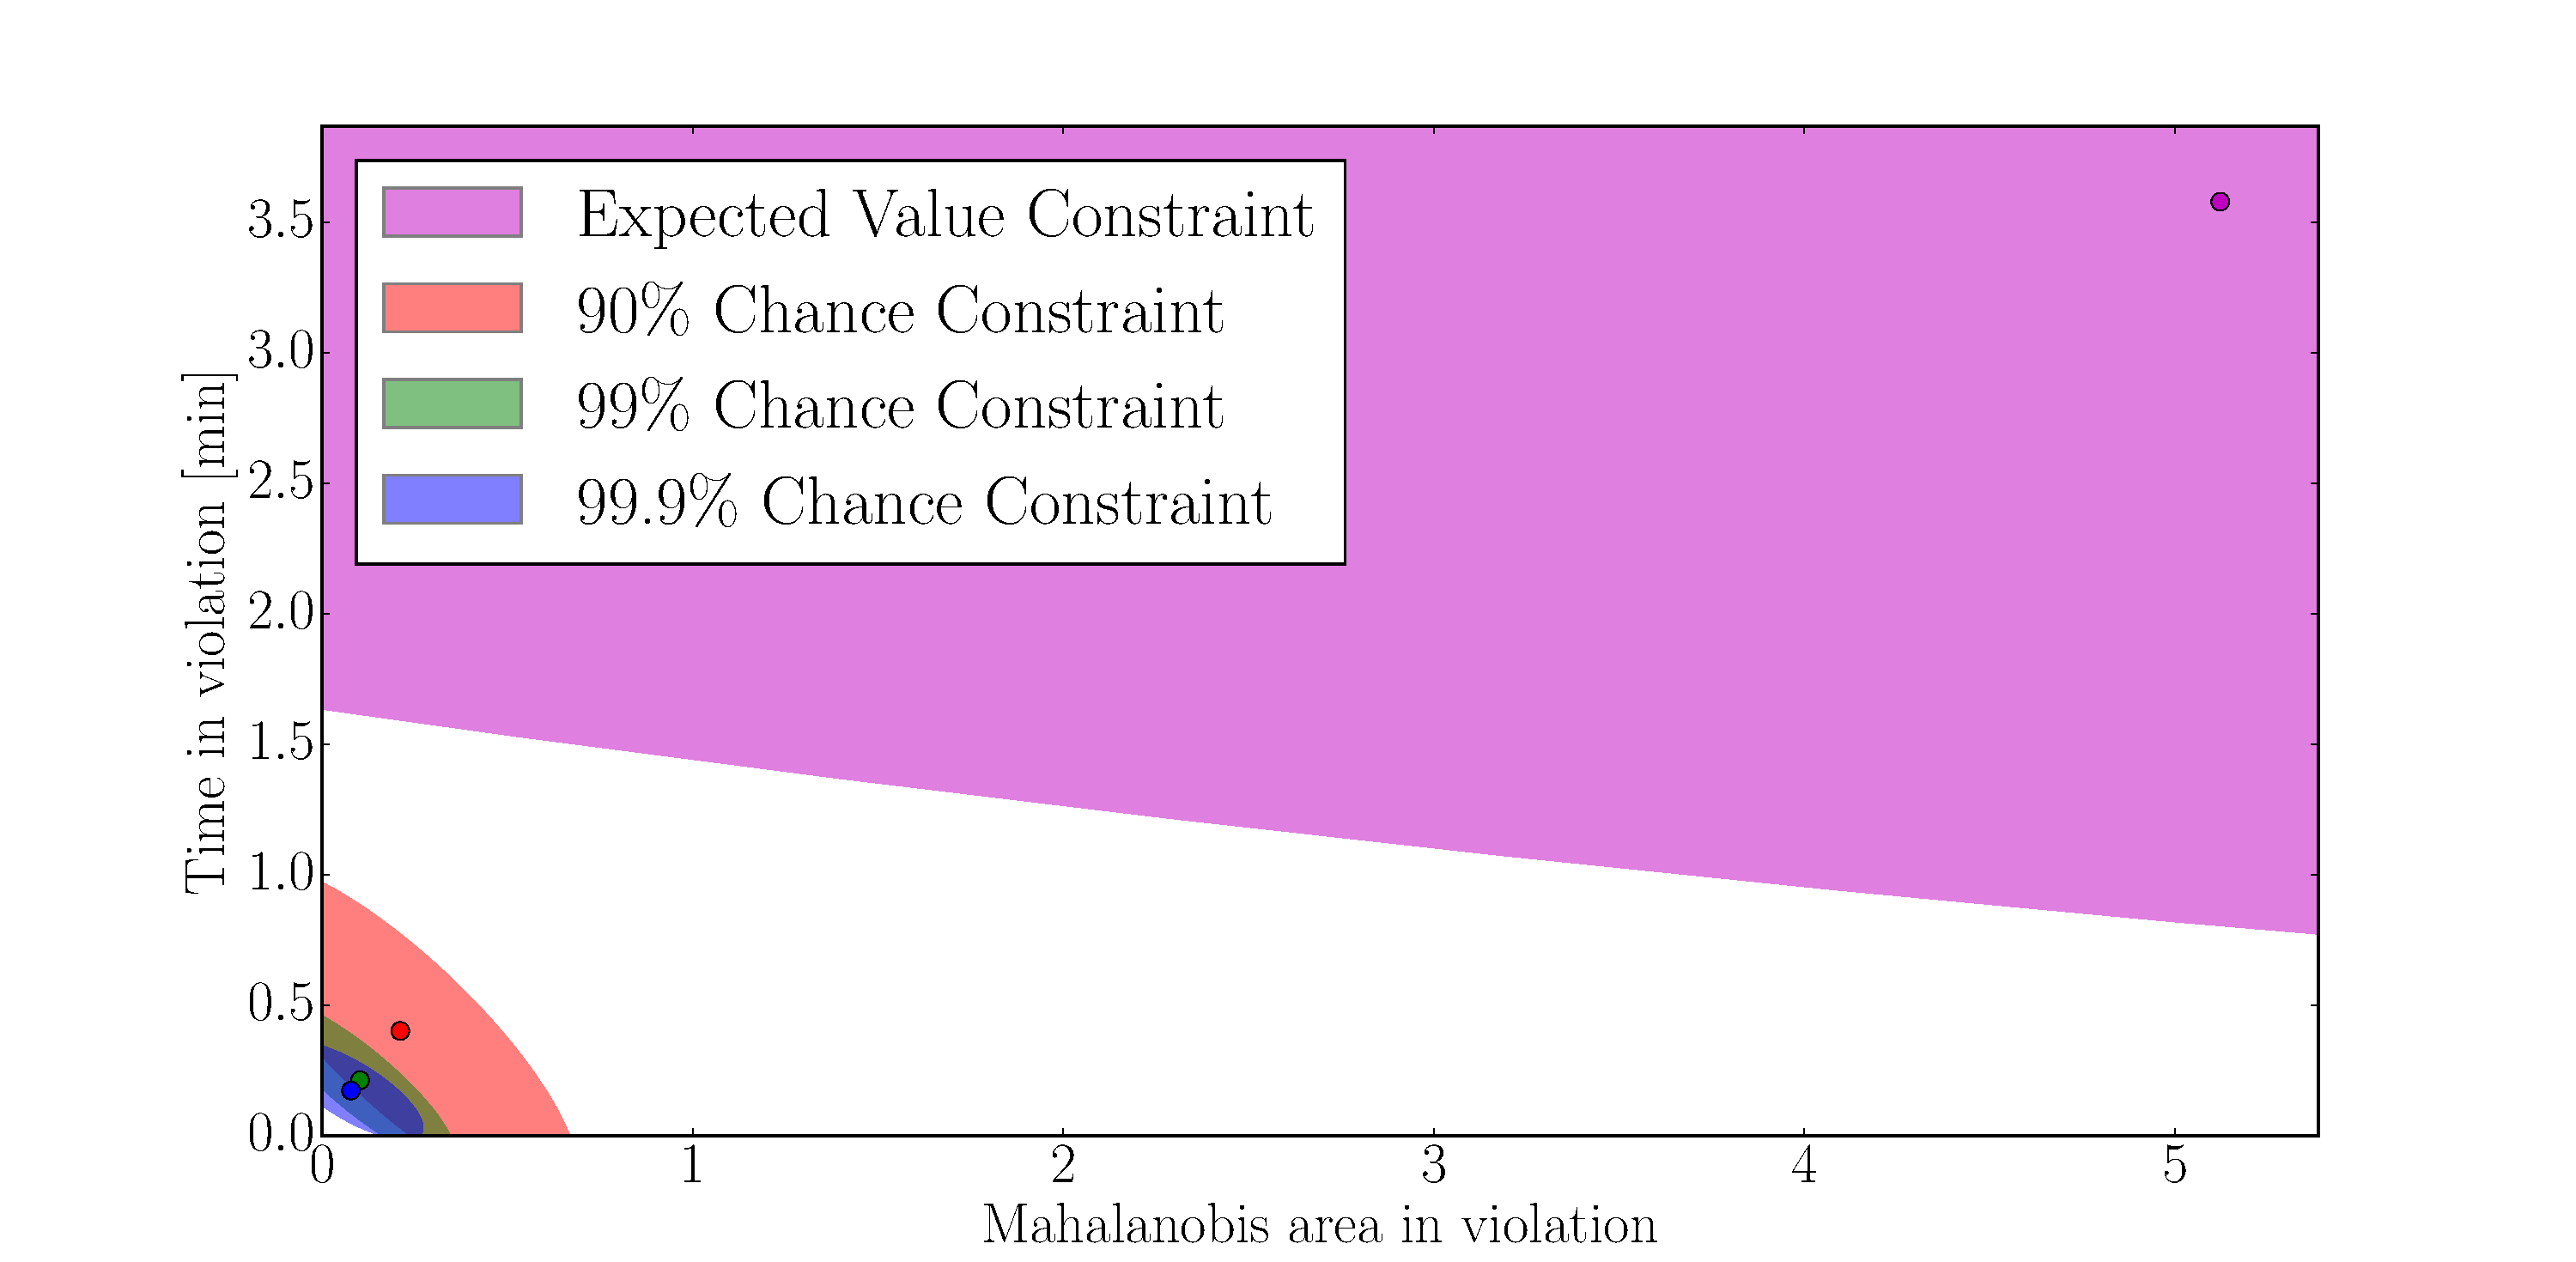
\includegraphics[width=\textwidth]{nonlin_mod_kf_mc.pdf}
\caption{Monte-Carlo simulation to investigate the effect increasing $k^2$ has on the constraint violation characteristics of the MPC controllers. Each region indicates where 90\% of the simulations scored. The mean is indicated by a solid point.}
\label{fig_nonlin_mod_kf_mc}
\end{figure}
It is clear that increasing $k^2$ causes the constraints to be violated less. It is also clear that the expected value constrained MPC (i.e. the deterministic MPC) performed significantly worse with the nonlinear underlying model when compared to Figure \ref{fig_lin_mod_kf_mc}. The value of the chance constrained MPC is apparent here. Unlike Figure \ref{fig_lin_mod_kf_mc} there seems to be more value in increasing the chance threshold above the 99\% interval.

Figures \ref{fig_nonlin_mod_kf_var90_track} to \ref{fig_nonlin_mod_kf_var99_ss} all display the undesirable property originally seen in Figure \ref{fig_nonlin_mod_kf_mean_track}: the poor state estimation and associated control problems. We attempt to rectify this situation by using a more sophisticated filter with the chance constrained MPC. We use the MPC as shown in (\ref{eq_mpc_nonlin_mod_cons}) with a particle filter using 200 particles. The tracking results are shown in Figure \ref{fig_nonlin_mod_pf_mean_track}. 
\begin{figure}[H] 
\centering
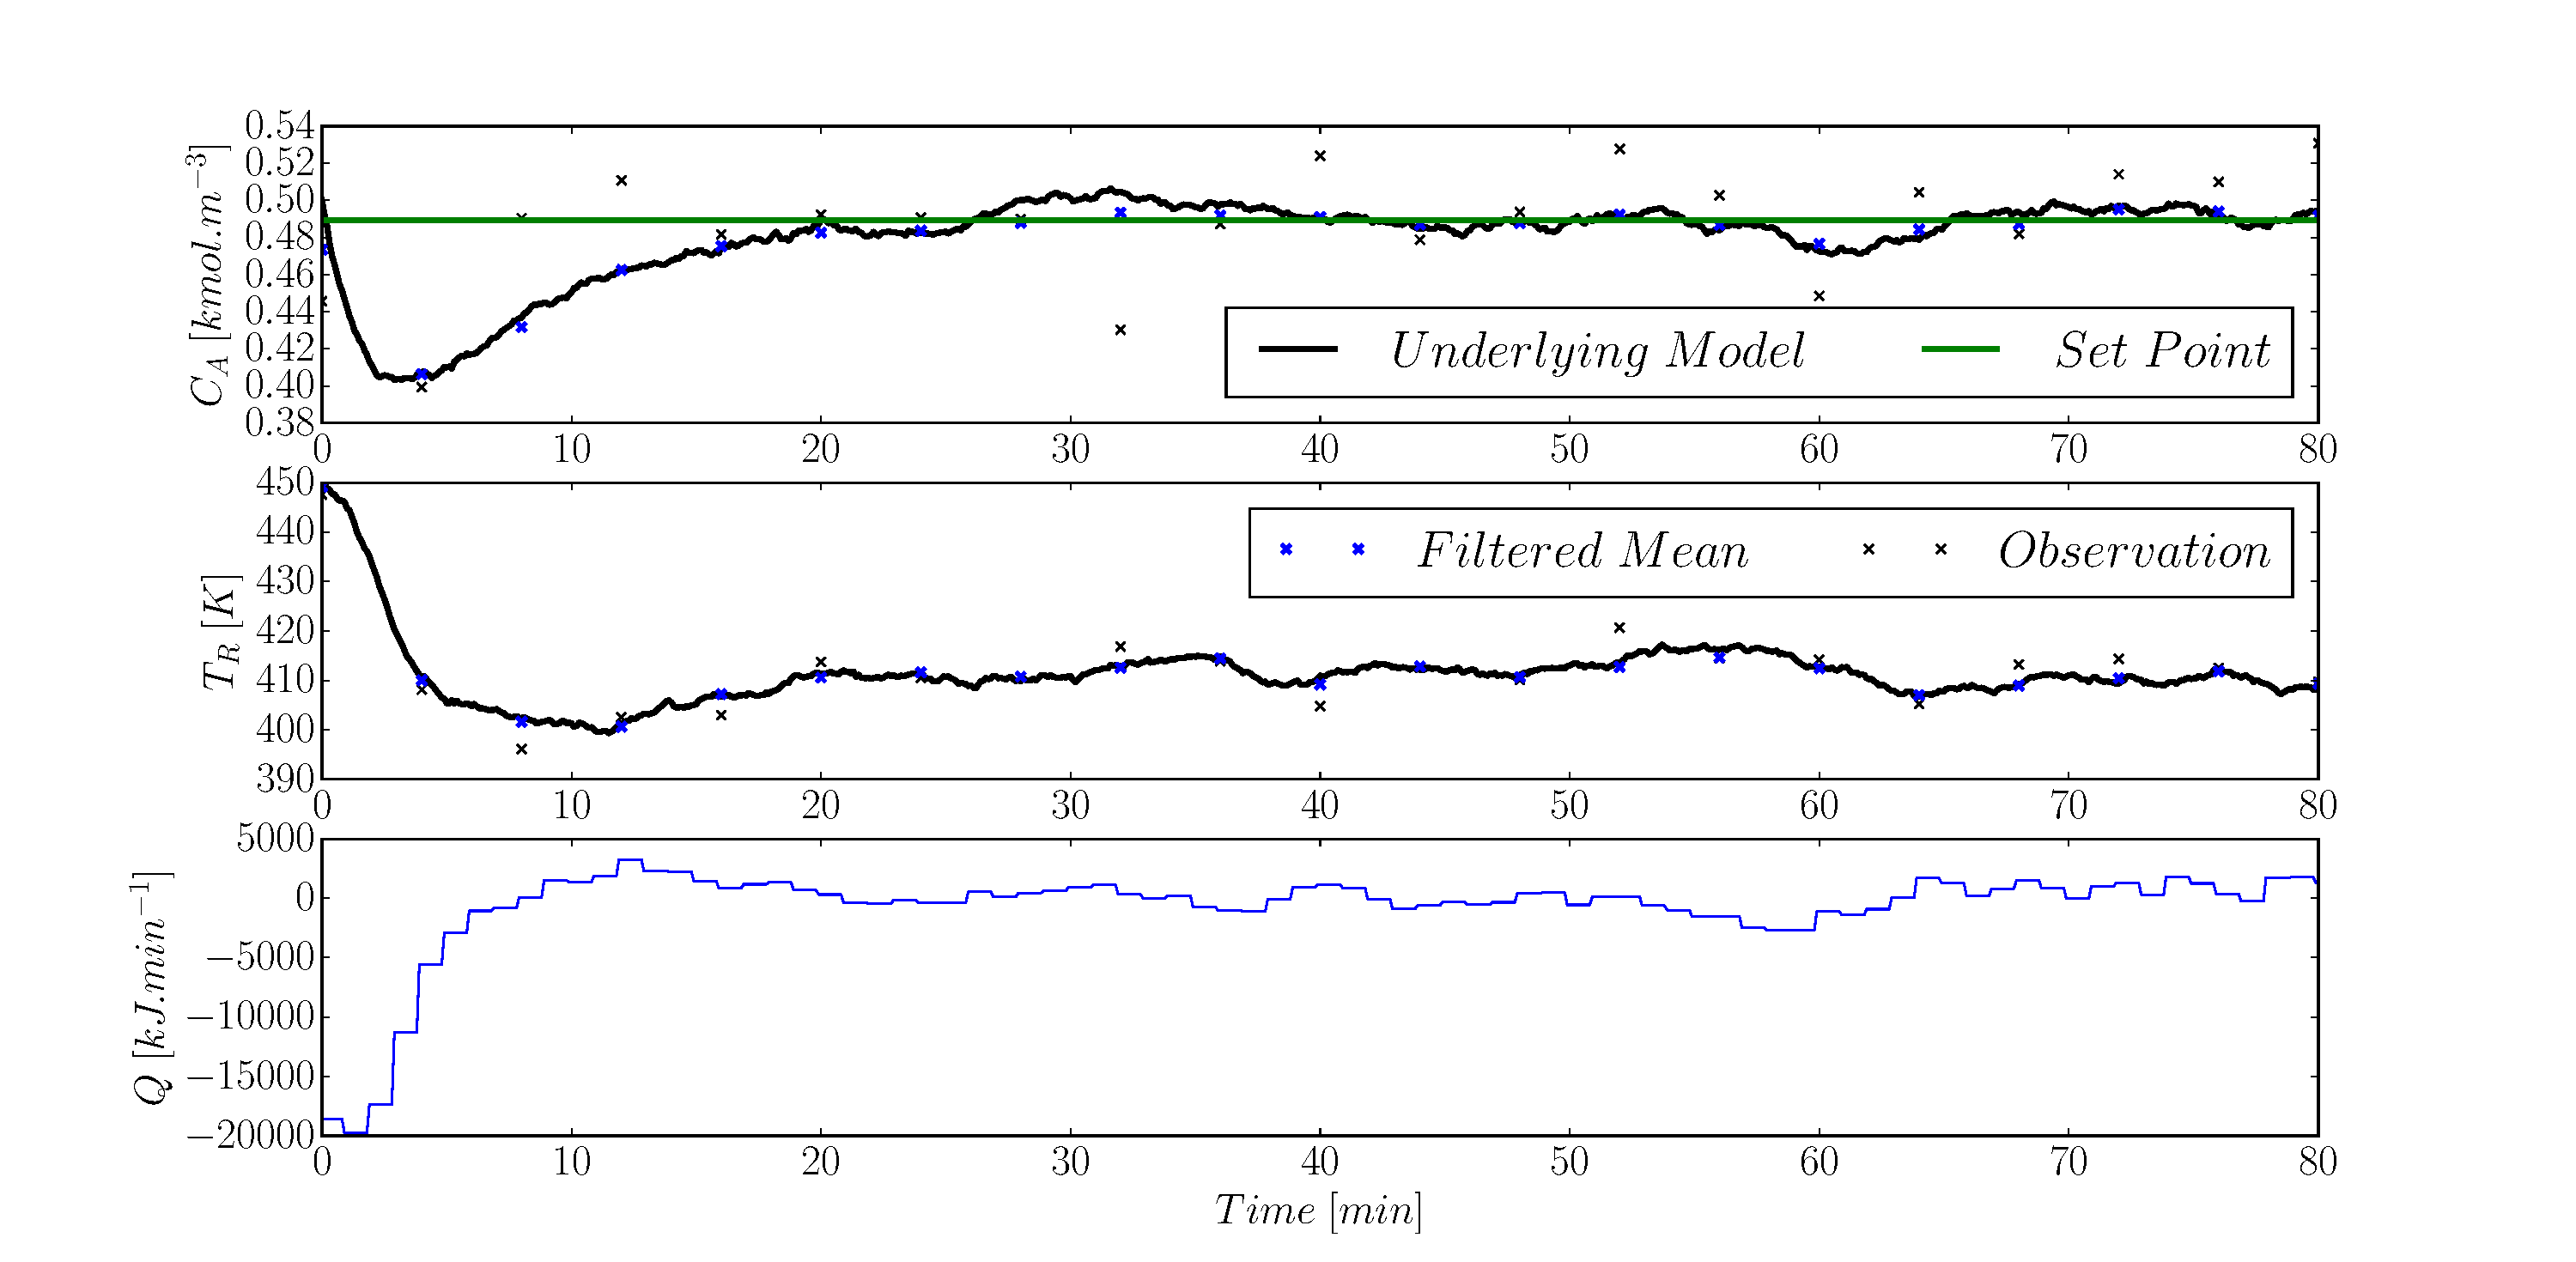
\includegraphics[width=\textwidth]{nonlin_mod_pf_var90_track.pdf}
\caption{Chance constrained MPC tracking with initial condition $(0.55, 450)$ and measuring both states. A particle filter with 200 particles is used for inference and the chance constraint is set at 90\%.}
\label{fig_nonlin_mod_pf_var90_track}
\end{figure}
One could see the discussion in Chapter \ref{sec_nonlinmods_filtering} as a justification for using the particle filter instead of the Kalman filter for state estimation. Since the underlying model is non-linear we expect the particle filter to outperform the Kalman filter (recall the discussion following Figure \ref{fig_pf_kf_phase2}).

The average input energy and average concentration error is 24.26 kW and 2.34\% over the course of the simulation. This is a vast improvement over the Kalman filter MPC combination. Clearly the more accurate state estimation is immensely beneficial for control. Figure \ref{fig_nonlin_mod_pf_var90_ss} also illustrates that the chance constraint is easily satisfied using the more accurate state estimator.
\begin{figure}[H] 
\centering
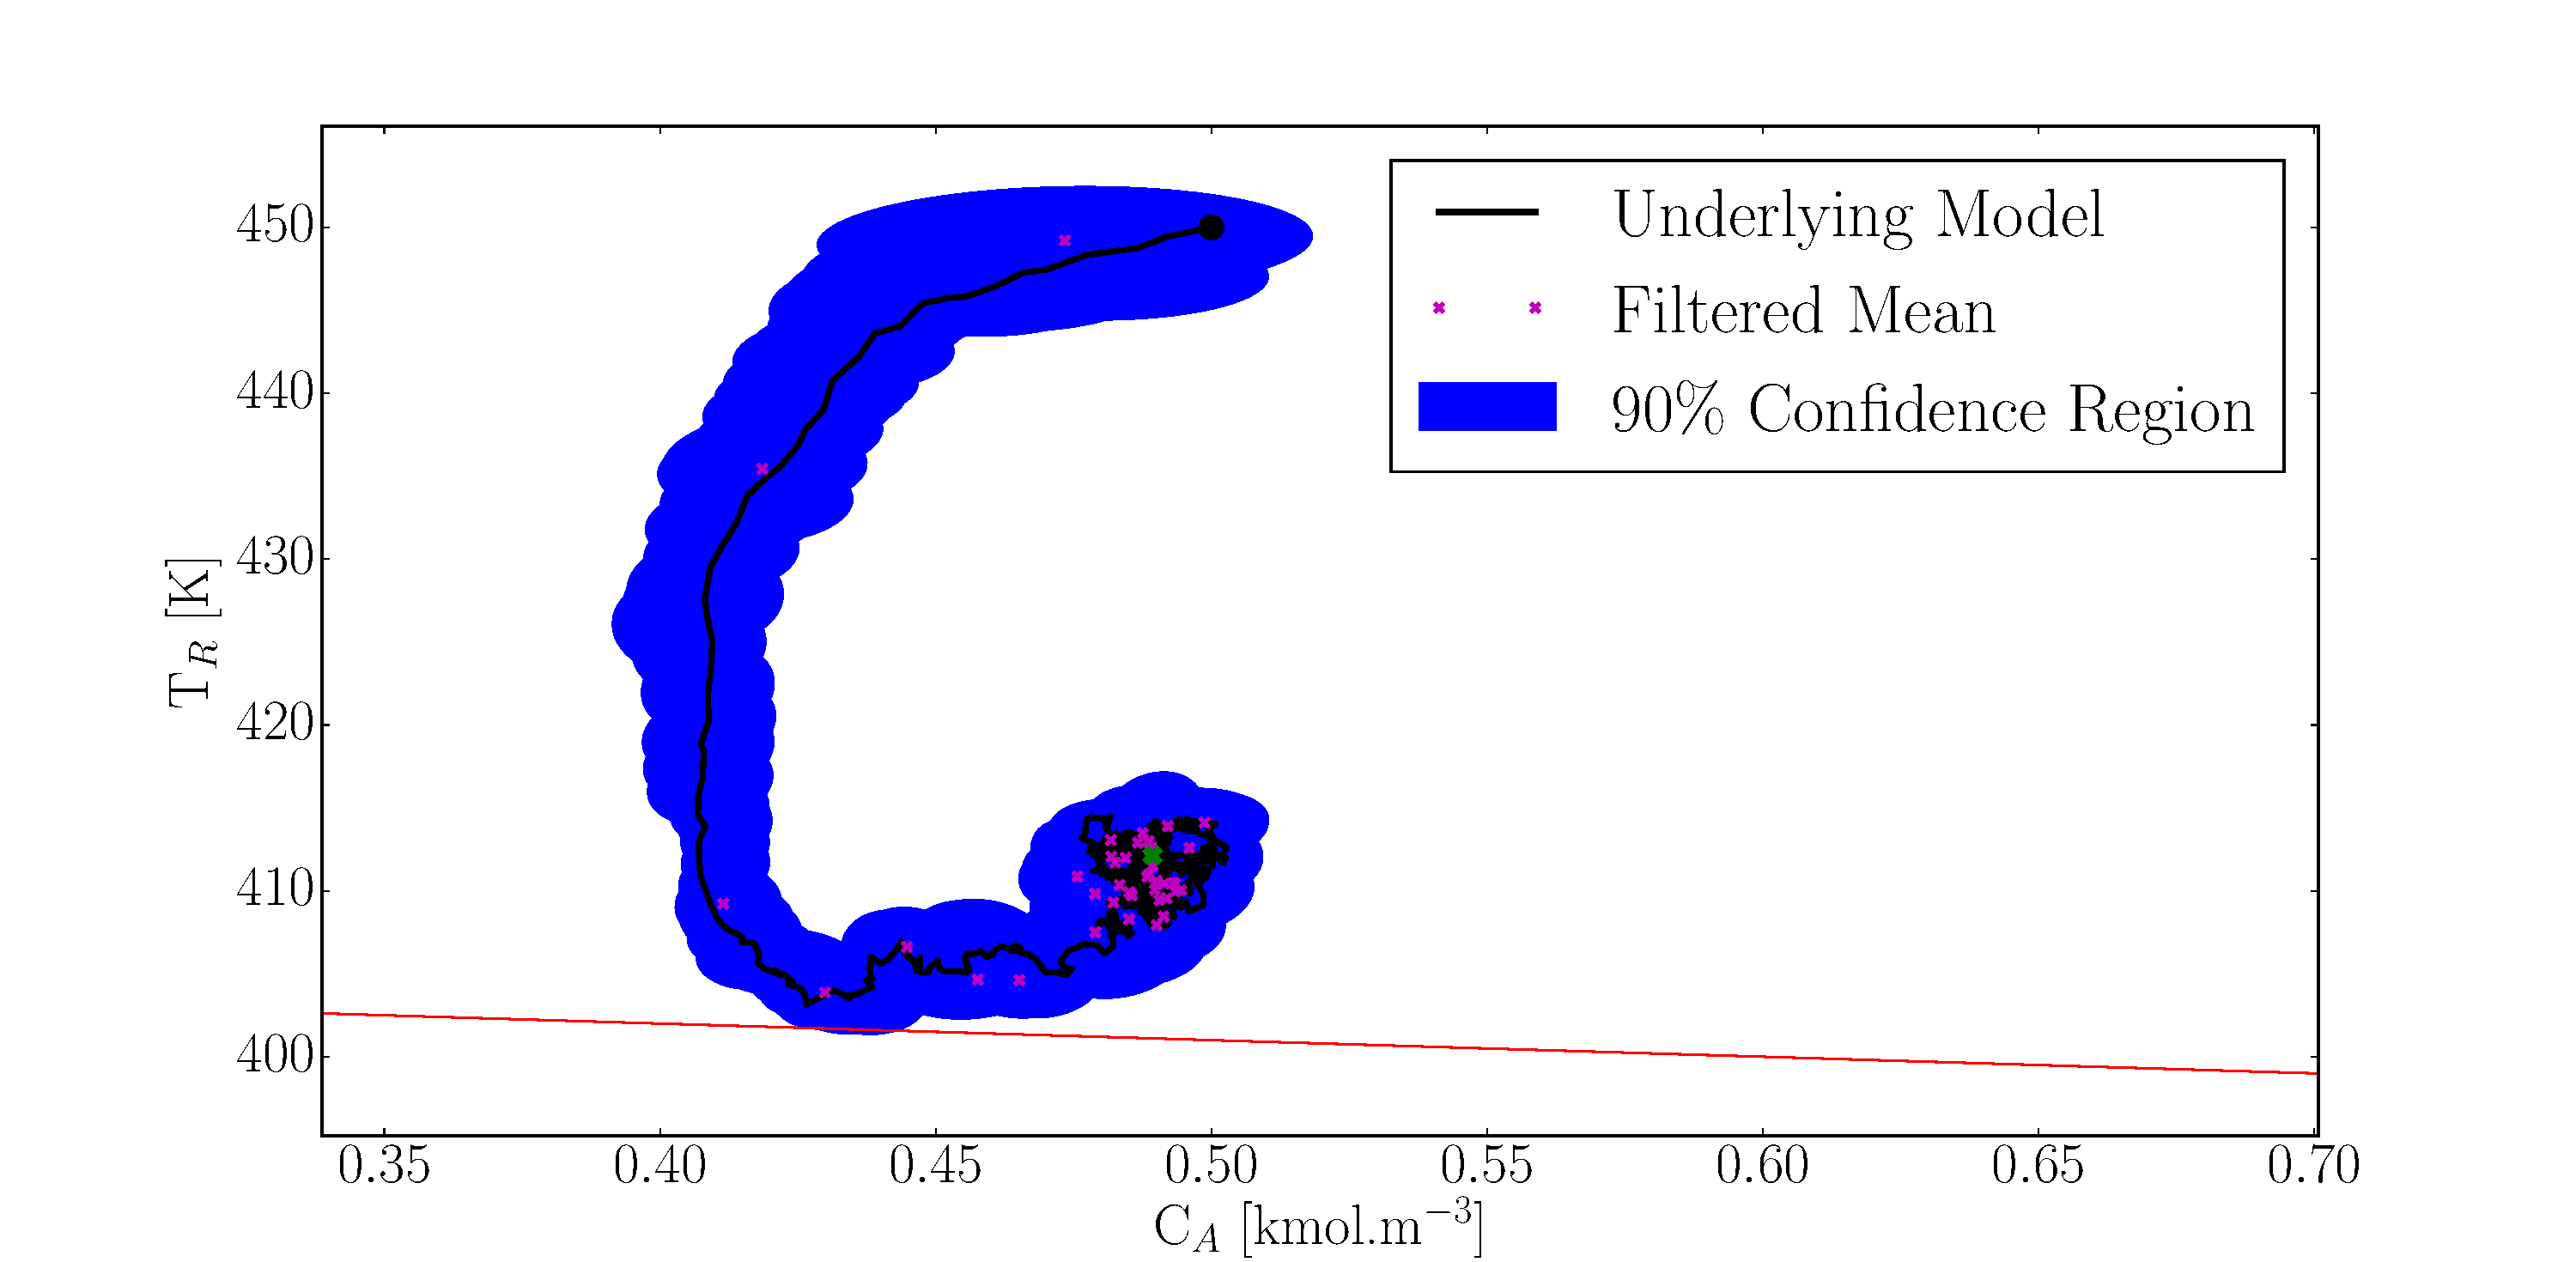
\includegraphics[width=\textwidth]{nonlin_mod_pf_var90_ss.pdf}
\caption{Chance constrained MPC state space trajectory with initial condition $(0.55, 450)$ and measuring both states. A particle filter with 200 particles is used for inference and the chance constraint is set at 90\%.}
\label{fig_nonlin_mod_pf_var90_ss}
\end{figure}
In Figure \ref{fig_nonlin_mod_pf_mc} we compare the constraint violation characteristics of the Kalman filter and particle filter based MPCs using over 2000 simulations. 
\begin{figure}[H] 
\centering
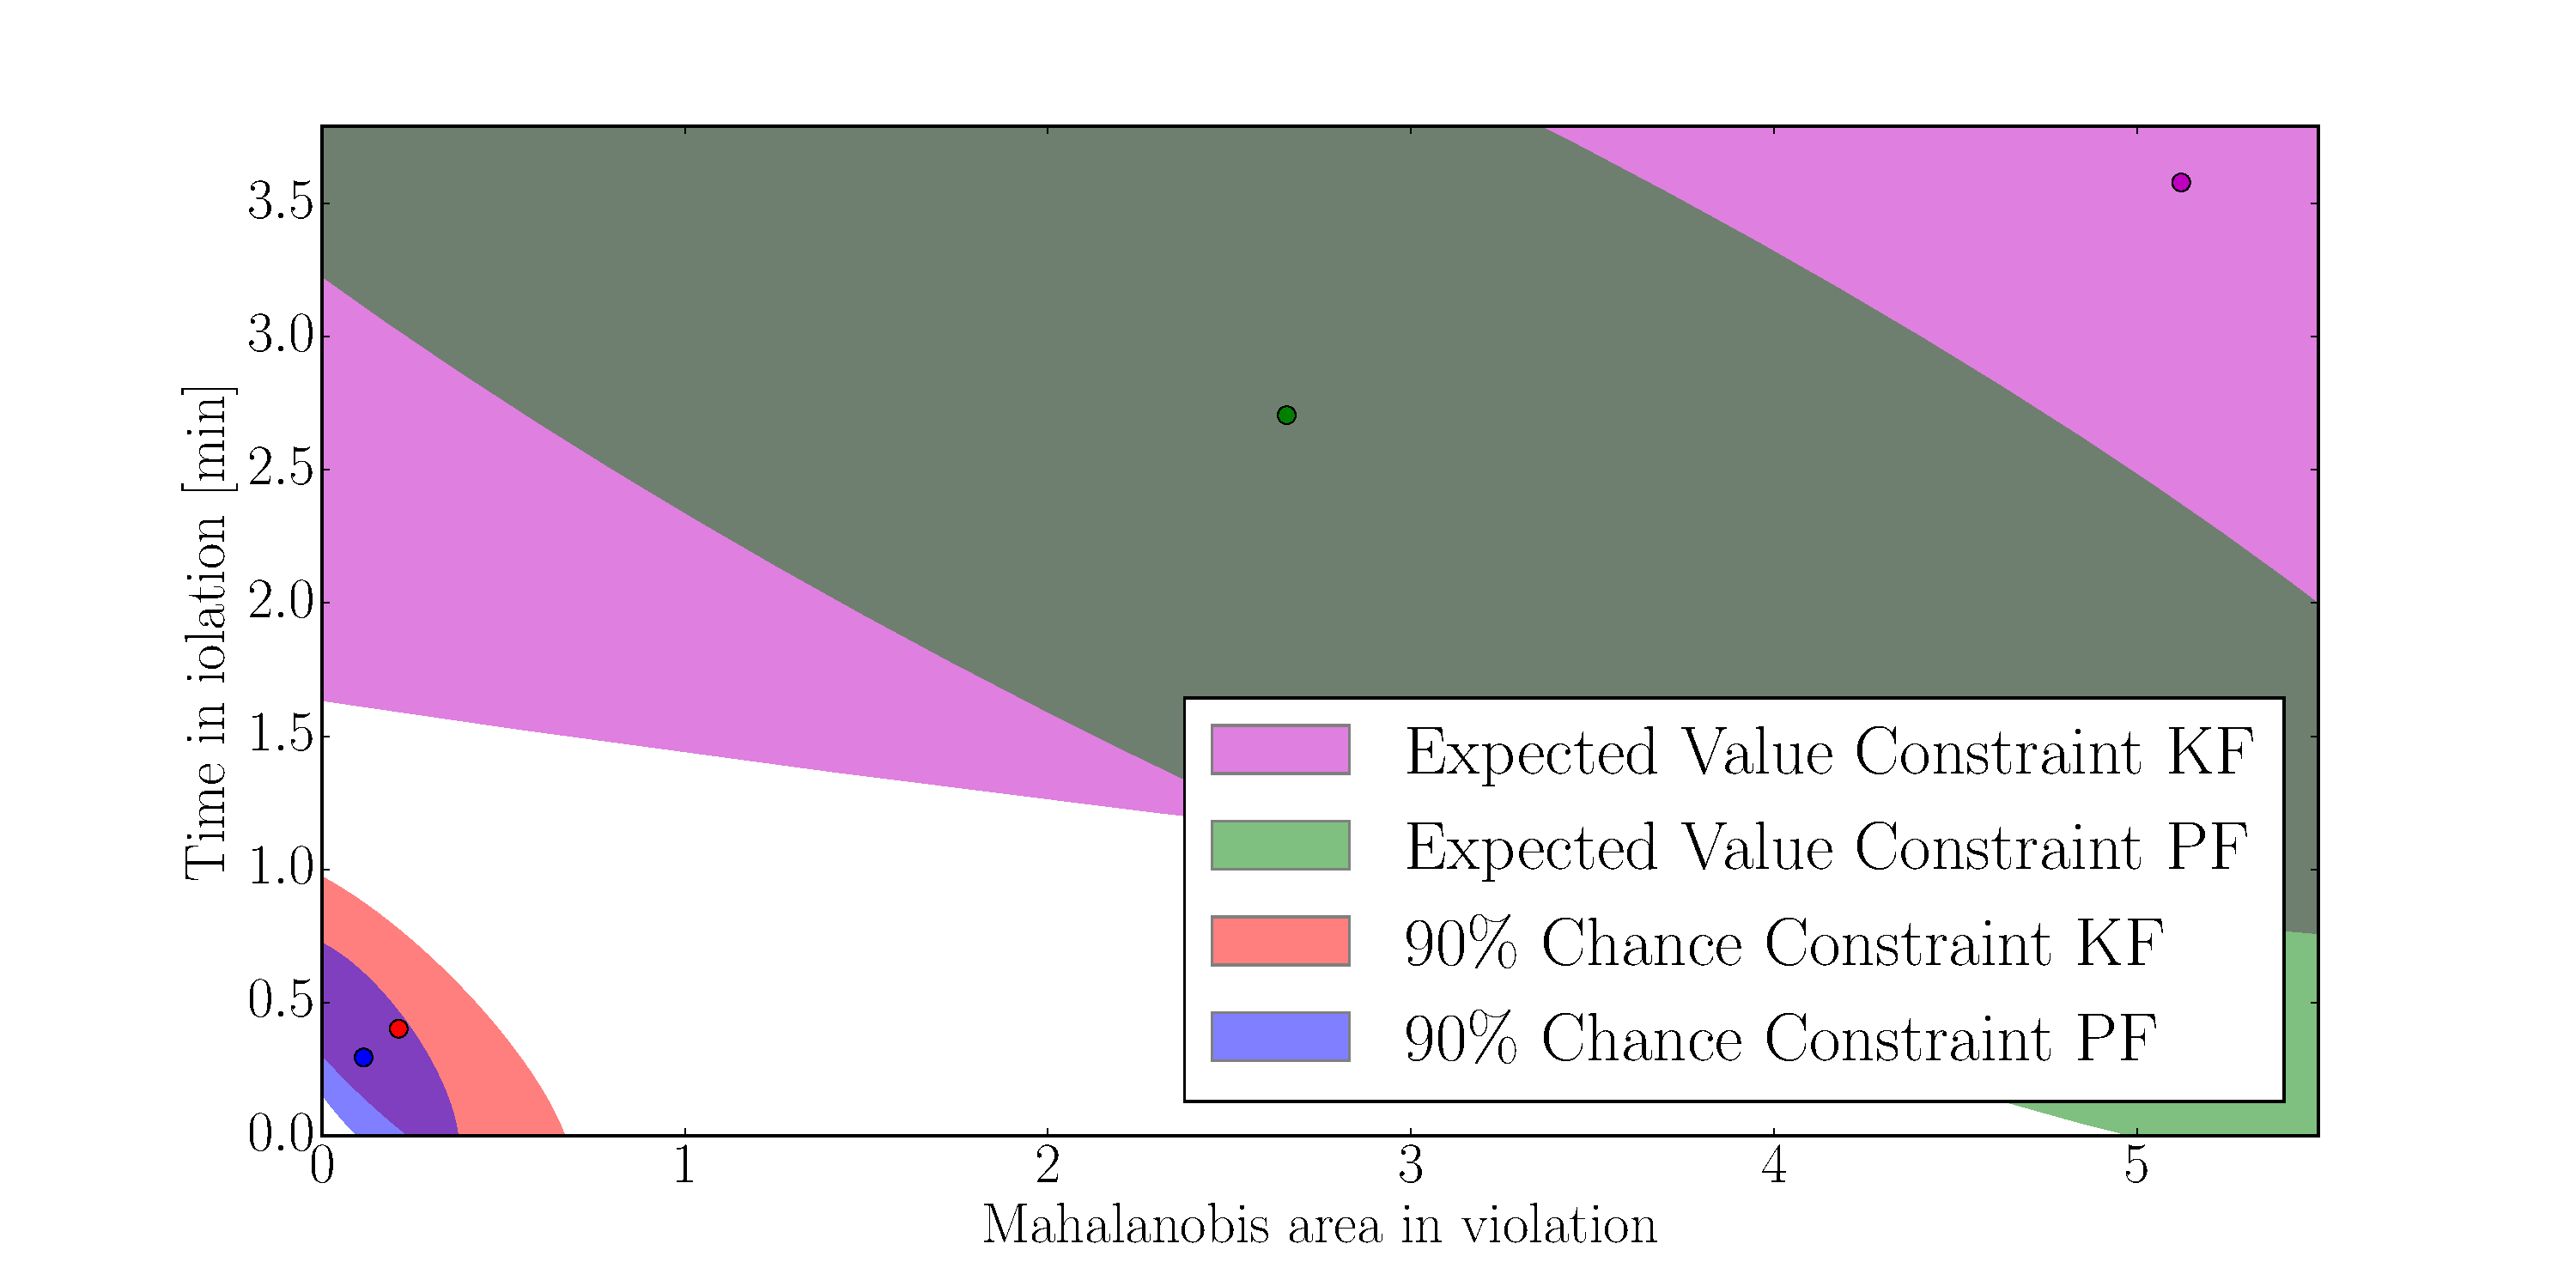
\includegraphics[width=\textwidth]{nonlin_mod_kf_pf_mc.pdf}
\caption{Monte-Carlo simulation to investigate the effect increasing $k^2$ has on the constraint violation characteristics of the MPC controllers. Each region indicates where 90\% of the simulations scored. The mean is indicated by a solid point. KF indicates the Kalman Filter MPC and PF indicates the particle filter MPC.}
\label{fig_nonlin_mod_pf_mc}
\end{figure}
It is clear that the particle filter based MPC outperforms the Kalman filter based MPC. This is not surprising because, as we discussed for the single realisation results, the state estimation ability of the Kalman filter is inferior due to the nonlinear underlying system.

As before we need to investigate the normal assumption underpinning the theory behind the chance constraint simplification. We investigate it in exactly the same manner as Figure \ref{fig_lin_mod_kl} using Kullback-Leibler Divergence. To this end, Figure \ref{fig_nonlin_mod_kl} shows the degree to which the underlying posterior state distributions are Gaussian given the non-linear underlying system.
\begin{figure}[H] 
\centering
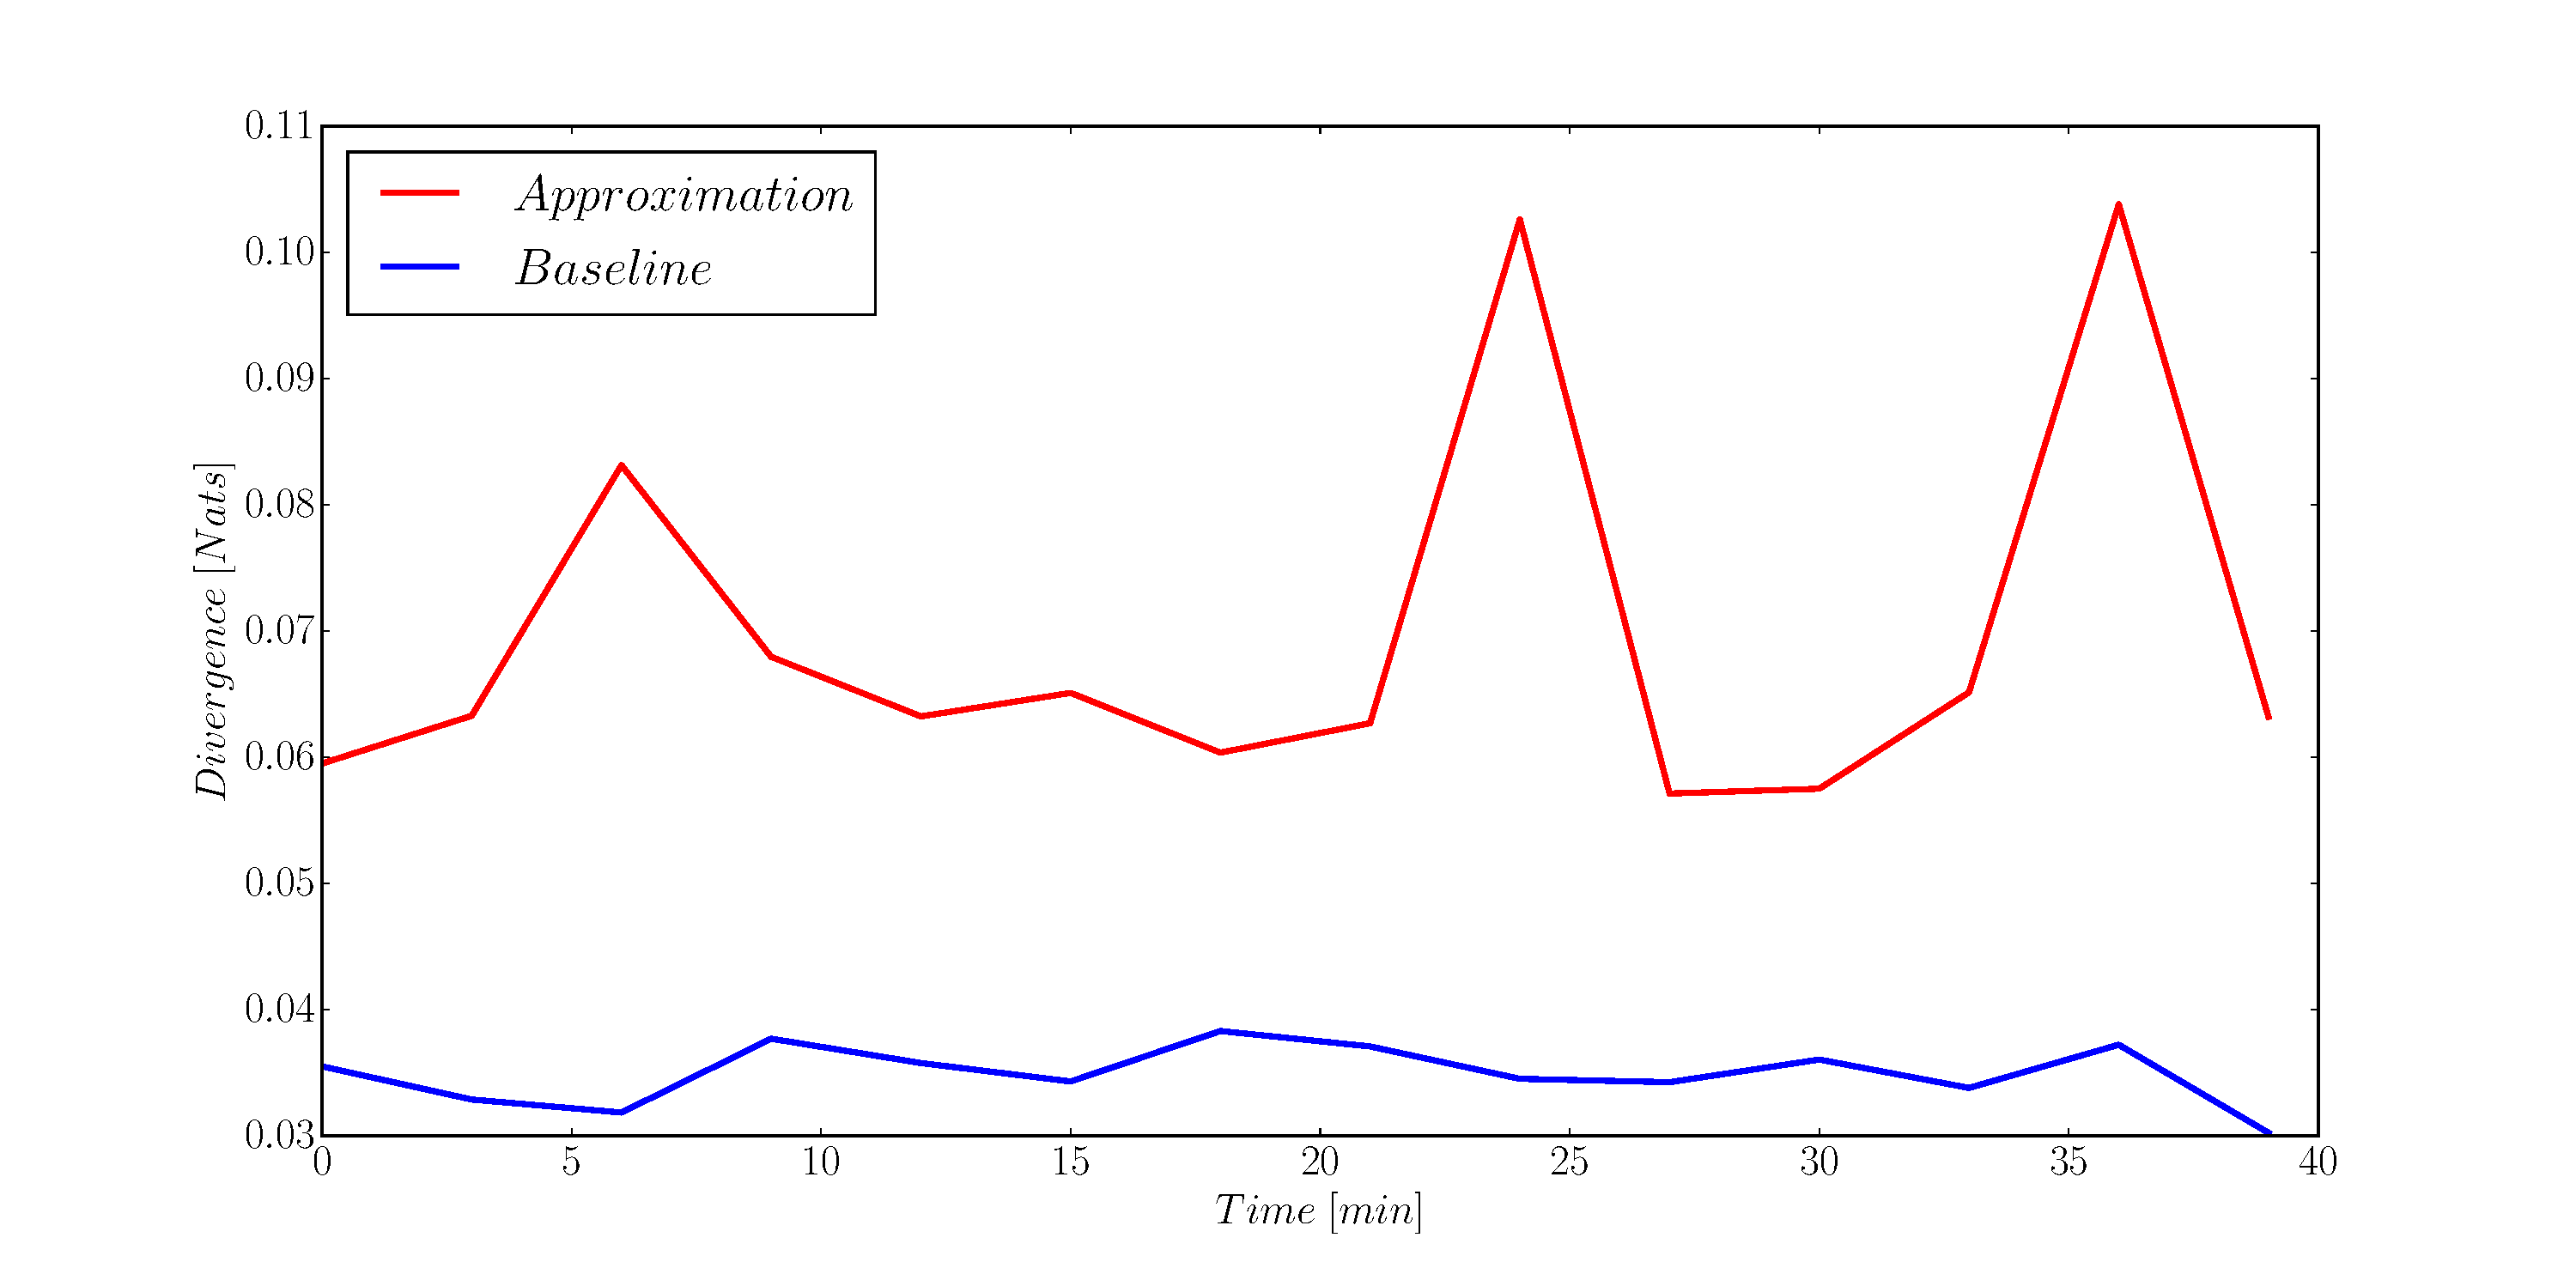
\includegraphics[width=\textwidth]{nonlin_mod_kl.pdf}
\caption{Kullback-Leibler Divergence between the assumed Gaussian distribution and actual distribution using 5000 particles. The underlying model is non-linear.}
\label{fig_nonlin_mod_kl}
\end{figure}
It is a relief that the normal assumption seems to hold almost as well in the non-linear underlying system case. The average divergence for the baseline, approximation and uniform curves are: $0.035$, $0.071$ and $0.324$. It is not surprising that the underlying nonlinearity reduced the degree of normality of the distributions. However, the distribution were not significantly non-Gaussian to raise any concern - the difference between Figures \ref{fig_lin_mod_kl} and \ref{fig_nonlin_mod_kl} is almost negligible.

\section{Conclusion}
We have illustrated the benefits gained by designing model predictive controllers within the framework of probabilistic graphical models by showing:
\begin{enumerate}
\item
Under the assumption of normality and linearity it is possible to convert stochastic quadratic objective functions into their deterministic equivalents. The analysis is closely related to the work of \cite{yan1} and \cite{yan2} but we have shown that these results are immediately obvious from within the framework of probabilistic graphical models. Thus it is possible to solve LQG objective type problems without resorting to stochastic dynamic programming.
\item
We have generalised our analysis to stochastic MPC and shown that by using the statistically important metric, the Mahalanobis distance, we arrive at a technique for enforcing chance constraints which is very closely related to the approach taken by \cite{vanhessem2} and \cite{vanhessem1}. Under the assumptions of linearity and normality we have shown that constraint satisfaction is ensured. Due to the use of the Mahalanobis distance metric we have provided some theoretical support for the use of the ``ellipsoidal approximation" technique if the underlying system is nonlinear or not exactly Gaussian.
\item
Combining the previous results we have shown that it is possible to write the joint chance constrained stochastic quadratic MPC problem as a deterministic quadratic MPC problem. Additionally we show that the joint chance constraints can be written in a linear format. The entire optimisation problem can then be written in the standard form for quadratic programming optimisation. Standard deterministic MPC solution and analysis techniques can then be used to solve the stochastic problem.
\item
We have compared the effect different inference techniques have on the quality of the MPC. If the system is linear and Gaussian the Kalman filter is adequate. If there is significant departure from linearity or normality it can be beneficial to use the particle filter.
\end{enumerate}